\documentclass[b5paper,11pt,twoside,openleft]{memoir}
\usepackage[left=1in,right=1.15in,top=1.25in,bottom=1.15in]{geometry}
\usepackage{xltxtra}
\usepackage{unicode-math}
\usepackage[greek]{babel}
\usepackage{listings}
\usepackage{xcolor}
\begin{document}
\setmainfont[Mapping=tex-text,Ligatures=Common]{Calibri}
\setsansfont[Mapping=tex-text,Scale=MatchLowercase]{Candara}
\setmonofont[Mapping=tex-text,Scale=MatchLowercase]{Consolas}
\setmathfont{Cambria Math}
\newtheorem{theorem}{Theorem}[section]
\newtheorem{exercise}[theorem]{Άσκηση}
\NewDocumentCommand\sel{om}{%
  \IfNoValueTF{#1}
    {(Στο βιβλίο βρίσκεται στη Σελ. #2)}%
    {(Άσκηση #1 του βιβλίου, Σελ. #2)}
}
\definecolor{background}{RGB}{248, 248, 242}
\definecolor{string}{RGB}{39, 40, 34}
\definecolor{comment}{RGB}{117, 113, 94}
\definecolor{normal}{RGB}{39, 40, 34}
\definecolor{identifier}{RGB}{166, 226, 46}

\lstset{
  language=python,                			% choose the language of the code
  numbers=left,                   		% where to put the line-numbers
  stepnumber=1,                   		% the step between two line-numbers.        
  numbersep=5pt,                  		% how far the line-numbers are from the code
  backgroundcolor=\color{background},  		% choose the background color. You must add \usepackage{color}
  showspaces=false,               		% show spaces adding particular underscores
  showstringspaces=false,         		% underline spaces within strings
  showtabs=false,                 		% show tabs within strings adding particular underscores
  tabsize=4,                      		% sets default tabsize to 2 spaces
  captionpos=b,                   		% sets the caption-position to bottom
  breaklines=true,                		% sets automatic line breaking
  breakatwhitespace=true,         		% sets if automatic breaks should only happen at whitespace
  title=\lstname,                 		% show the filename of files included with \lstinputlisting;
  basicstyle=\color{normal},					% sets font style for the code
  keywordstyle=\color{magenta},	% sets color for keywords
  stringstyle=\color{string},		% sets color for strings
  commentstyle=\color{comment},	% sets color for comments
  emph={format_string, eff_ana_bf, permute, eff_ana_btr},
  emphstyle=\color{identifier},
  escapeinside={(@*}{*@)},
  columns = fullflexible}
\title{%
%$A\lambda\gamma\epsilon\beta\rho y$ \\ 
Μαθηματικά Γυμνασίου με Python}

\author{}
\maketitle
\chapter*{Εισαγωγή}
Το βιβλίο αυτό είναι ένας συνδυασμός των μαθηματικών που έμαθες στην Α΄ Γυμνασίου με τη γλώσσα προγραμματισμού Python. Θα θυμηθείς όσα έμαθες στην Α΄ Γυμνασίου και θα μάθεις και τα βασικά μιας σύγχρονης γλώσσας προγραμματισμού που χρησιμοποιείται από πολλούς προγραμματιστές σε όλον τον κόσμο.

Για να εγκαταστήσεις την Python στον υπολογιστή σου πήγαινε στη σελίδα https://www.python.org/ και κατέβασε την τελευταία έκδοση της Python 3 (Latest). Αφού κάνεις εγκατάσταση θα βρεις στον υπολογιστή σου το πρόγραμμα IDLE με το οποίο μπορείς να δουλέψεις αυτές τις σημειώσεις.

\chapter{Φυσικοί αριθμοί}

\section{Οι αριθμοί και η Python}

Οι φυσικοί αριθμοί είναι οι αριθμοί από 0, 1, 2, 3, 4, 5, 6, \ldots, 98, 99, 100, \ldots, 1999, 2000, 2001, \ldots

Η Python μπορεί να χειριστεί φυσικούς αριθμούς. Δοκιμάστε να γράψετε στο REPL έναν φυσικό αριθμό, θα δεις ότι η Python θα τον επαναλάβει. Π.χ. δες τον αριθμό εκατόν είκοσι τρια (123).
\begin{lstlisting}
>>> 123
123
\end{lstlisting}

Στην Python όμως θα πρέπει να ακολουθείς κάποιους επιπλέον κανόνες. Για παράδειγμα στους αριθμούς δεν πρέπει να βάζεις τελείες στις χιλιάδες όπως στο χαρτί. Αν το κάνεις στην καλύτερη περίπτωση θα προκύψει κάποιο λάθος, στην χειρότερη ο υπολογιστής θα καταλάβει διαφορετικό αριθμό από αυτόν που εννοείς.
Δες το παρακάτω παράδειγμα:
\begin{lstlisting}
>>> 1.000.000
  File "<stdin>", line 1
    1.000.000
            ^
SyntaxError: invalid syntax
>>> 100.000
100.0
\end{lstlisting}
Σε αυτό το παράδειγμα, η Python δεν καταλαβαίνει καθόλου τον αριθμό 1.000.000 γραμμένο με τελείες ενώ μεταφράζει το 100.000 σε 100.0, που για την Python σημαίνει 100 (εκατό). Γι' αυτόν τον λόγο δεν βάζουμε καθόλου τελείες έτσι αν θέλουμε να γράψουμε το ένα εκατομμύριο θα γράψουμε 1000000.
\begin{lstlisting}
>>> 1000000
1000000
\end{lstlisting}

\section{Πρόσθεση, αφαίρεση και πολλαπλασιασμός φυσικών αριθμών}
Μια γλώσσα προγραμματισμού μπορεί να εκτελέσει απλές πράξεις πολύ εύκολα. Στο βιβλίο των μαθηματικών  σου μπορείς να βρεις πολλές ασκήσεις με πράξεις. Μπορείς να τις λύσεις με την Python.

\begin{exercise}
\sel{16}
Να υπολογιστούν τα γινόμενα: 

(α) $35 \cdot 10$, 

(β) $421 \cdot 100$,

(γ) $5 \cdot 1.000$,

(δ) $27 \cdot 10.000$
\end{exercise}

Η python μπορεί να κάνει αυτές τις πράξεις ως εξής:
\begin{lstlisting}
>>> 35*10
350
>>> 421*100
42100
>>> 5*1000
5000
>>> 27*10000
270000
\end{lstlisting}

Ο τελεστής του πολλαπλασιασμού είναι το αστεράκι * (SHIFT+8) στο πληκτρολόγιο. Εναλλακτικά, μπορείς να το βρείς στο αριθμητικό πληκτρολόγιο. 

\begin{exercise}
\sel{16}
Να εκτελεστούν οι ακόλουθες πράξεις:

(α) $89\cdot 7 + 89\cdot 3$

(β) $23 \cdot 49 + 77 \cdot 49$

(γ) $76 \cdot 13 – 76 \cdot 3$

(δ) $284 \cdot 99$
\end{exercise}
\begin{lstlisting}
>>> 89*7+89*3
890
>>> 23*49+77*49
4900
>>> 76*13-76*3
760
>>> 284*99
28116
\end{lstlisting}

Στις παραπάνω περιπτώσεις η python εκτελεί πρώτα τους πολλαπλασιασμούς και μετά τις προσθέσεις/αφαιρέσεις δίνοντας έτσι το αποτέλεσμα που αναμένεται. Για παράδειγμα 89\*7 + 89\*3 = 623 + 267 = 890, που είναι το σωστό αποτέλεσμα.

\begin{exercise}
\sel{18}
Υπολογίστε:

(α)  $157 + 33$ 

(β)  $122 + 25 + 78$

(γ)  $785 - 323$

(δ)  $7.321 - 4.595$

(ε)  $60 - (18 - 2)$

(στ) $52 - 11 -9$

(ζ)  $23 \cdot 10$

(η)  $97 \cdot 100$

(θ)  $879 \cdot 1.000$
\end{exercise}
Σε python τα παραπάνω υπολογίζονται ως εξής:
\begin{lstlisting}
>>> 157+33
190
>>> 122+25+78
225
>>> 785-323
462
>>> 7321-4595
2726
>>> 60-(18-2)
44
>>> 52-11-9
32
>>> 23*10
230
>>> 97*100
9700
>>> 879*1000
879000
\end{lstlisting}
Οι παρενθέσεις (SHIFT+9 και SHIFT+0) αλλάζουν τη σειρά των πράξεων. Οι πράξεις που είναι μέσα στην παρένθεση εκτελούνται πρώτες. Γι' αυτό το λόγο 60-(18-2)=60-16=44.

\begin{exercise}
\sel{18}
Σε ένα αρτοποιείο έφτιαξαν μία μέρα 120 κιλά άσπρο ψωμί, 135 κιλά χωριάτικο, 25 κιλά σικάλεως και 38 κιλά πολύσπορο. Πουλήθηκαν 107 κιλά άσπρο ψωμί, 112 κιλά χωριάτικο, 19 κιλά σικάλεως και 23 κιλά πολύσπορο. Πόσα κιλά ψωμί έμειναν απούλητα;
\end{exercise}
Με τις γνώσεις που έχουμε θα πρέπει να μετατρέψουμε το παραπάνω πρόβλημα σε μια αριθμητική παράσταση ώστε η python να μπορεί να την υπολογίσει, στη συγκεκριμένη περίπτωση η σωστή παράσταση είναι: $$(120-107)+(135-112)+(25-19)+(38-23)$$
\begin{lstlisting}
>>> (120-107)+(135-112)+(25-19)+(38-23)
57
\end{lstlisting}
και η απάντηση είναι 57 κιλά ψωμί.

\section{Δυνάμεις φυσικών αριθμών}
Ο τελεστής της python για τις δυνάμεις είναι ο **  (δυο φορές το αστεράκι). Δηλαδή, αν θέλουμε να υπολογίσουμε το $10^2$ θα γράψουμε 10**2, με όμοιο τρόπο μπορούμε να υπολογίσουμε και τις υπόλοιπες δυνάμεις. Δοκίμασε τα παρακάτω στο REPL.
\begin{lstlisting}
>>> 10**2
100
>>> 10**3
1000
>>> 10**4
10000
>>> 10**5
100000
>>> 10**6
1000000
\end{lstlisting}
Στη προτεραιότητα των πράξεων, οι δυνάμεις έχουν μεγλύτερη προτεραιότητα από τον πολλαπλασιασμό και την πρόσθεση. Οπότε όταν έχουμε και δυνάμεις σε μια παράσταση πρώτα γίνονται οι πράξεις στις παρενθέσεις, μετά οι δυνάμεις και μετά οι πολλαπλασιασμοί και οι προσθέσεις. Την ίδια σειρά ακολουθεί και η python για τον υπολογισμό των πράξεων.
\begin{exercise}
\sel{21}
Να εκτελεστούν οι πράξεις 

 1. $(2\cdot 5)^4+4\cdot (3+2)^2$

 2. $(2+3)^3 - 8\cdot 3^2$

\end{exercise}
Οι αντίστοιχες εκφράσεις είναι (2*5)**4+4*(3+2)**2 και (2+3)**3 - 8*3**2.

\begin{lstlisting}
>>> (2*5)**4+4*(3+2)**2
10100
>>> (2+3)**3 - 8*3**2
53
\end{lstlisting}
H 8*3**2 υπολογίζεται ως $8\cdot (3^2)$, δηλαδή $8\cdot 9 = 72$, αφού πρώτα γίνεται η δύναμη και μετά οι πολλαπλασιασμοί.

\begin{exercise}
Κάνε τις πράξεις: 
(α) $3\cdot 5^2$, 

(β) $3\cdot 5^2 + 2$, 

(γ) $3\cdot5^2 + 2^2$, 

(δ) $3\cdot 5 + 2^2$, 

(ε) $3\cdot(5 + 2)^2$.
\end{exercise}

Αυτές οι πράξεις μπορούν να γίνουν στο REPL.
\begin{lstlisting}
>>> 3*5**2
75
>>> 3*5**2 + 2
77
>>> 3*5**2 + 2**2
79
>>> 3*5 +2**2
19
>>> 3*(5 + 2)**2
147
\end{lstlisting}

\begin{exercise}
Κάνε τις πράξεις: 
(α) $3^2 +3^3 +2^3 +2^4$, 

(β) $(13-2)^ 4 + 5\cdot 3^2$
\end{exercise}

\begin{lstlisting}
>>> 3**2 +3**3 +2**3 +2**4
60
>>> (13-2)**4 + 5*3**2
14686
\end{lstlisting}

\begin{exercise}
Βρες τις τιμές των παραστάσεων: 

(α) $(6+5)^2$ και $6^2+5^2$, 

(β) $(3+6)^2$ και $3^2+6^2$.
\end{exercise}
\begin{lstlisting}
>>> (6+5)**2
121
>>> 6**2+5**2
61
>>> (3+6)**2
81
>>> 3**2+6**2
45
\end{lstlisting}


\section{Συγκρίσεις φυσικών αριθμών}
Μπορούμε να συγκρίνουμε αριθμούς στην Python χρησιμοποιώντας τους τελεστές == (πληκτρολογούμε δύο φορές το =) για την \emph{ισότητα}, > για το \emph{μεγαλύτερο} και < για το \emph{μικρότερο}. Επίσης μπορούμε να χρησιμοποιήσουμε >= για το \emph{μεγαλύτερο ή ίσο} και <= για το \emph{μικρότερο ή ίσο}, τέλος υπάρχει το != για το \emph{δεν είναι ίσο}. Μπορείς να δοκιμάσεις τα παρακάτω:
\begin{lstlisting}
>>> 123==123
True
>>> 123>123
False
>>> 123>122
True
>>> 123<123
False
>>> 123<124
True
>>> 123<=123
True
>>> 123<=124
True
>>> 123<=122
False
>>> 123>=123
True
>>> 123>=124
False
>>> 123>=122
True
>>> 122 != 123
True
>>> 122 != 122
False
\end{lstlisting}
Η Python επιστρέφει True (αληθές) όταν μία πρόταση ισχύει και False (ψευδές) όταν δεν ισχύει.

Σκέψου ότι για την Python η σύγκριση είναι και αυτή μια πράξη. Αντί η πράξη αυτή να δίνει σαν αποτέλεσμα έναν αριθμό δίνει σαν αποτέλεσμα το αληθές ή το ψευδές.

Για παράδειγμα:
\begin{exercise}
Να συγκρίνετε τα $3^2$ και $2^3$.
\end{exercise}
Η σύγκριση αυτή μπορεί να γίνει στο REPL. Δοκίμασε:
\begin{lstlisting}
>>> 3**2 > 2**3
True
\end{lstlisting}
Άρα το $3^2$ είναι μεγαλύτερο από το $2^3$. Θυμήσου ότι το $3^2=9$, ενώ $2^3=8$.

\section{Η εντολή print}
Ήρθε η ώρα να γράψεις εντολές στο πάνω παράθυρο, δηλαδή να γράψεις το πρώτο σου πρόγραμμα.  Με βάση όσα ξέρεις προσπάθησε να γράψεις μια πράξη στο πάνω παράθυρο, για παράδειγμα $32+35$. Ύστερα πάτησε το κουμπί της εκτέλεσης (Run). Μπορείς να δεις το αποτέλεσμα στην εικόνα \ref{noprint}.
\begin{figure}
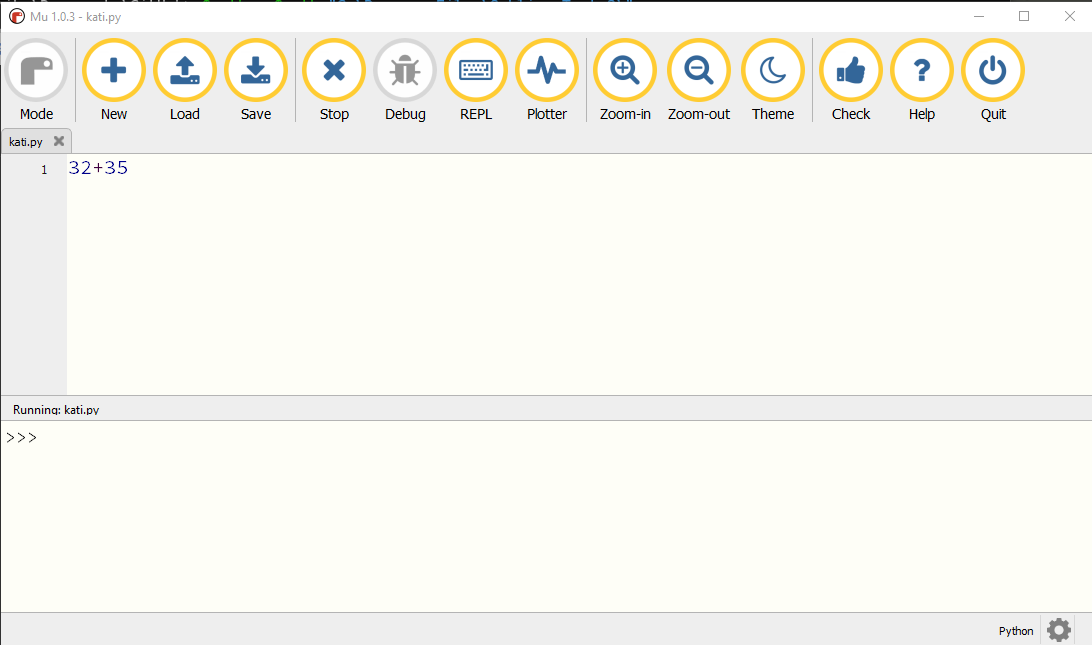
\includegraphics[width=\textwidth]{noprint.png}
\caption{Η εκτέλεση δεν δίνει κάποιο αποτέλεσμα}
\label{noprint}
\end{figure}

Η Python εκτελεί την πράξη $32+35$, και υπολογίζει το αποτέλεσμα. Αν δεν το έκανε και υπήρχε κάποιο πρόβλημα θα εμφάνιζε κάποιο μήνυμα λάθους στο REPL. Το υπολογισμένο αποτέλεσμα δεν εμφανίζεται. Για να εμφανιστεί το αποτέλεσμα πρέπει να χρησιμοποιήσεις την εντολή print (εκτύπωσε). Η εντολή print εκτελείται ως εξής:
\begin{lstlisting}
print(32+35)
\end{lstlisting}
Γράφουμε δηλαδή, print ανοίγουμε παρένθεση, γράφουμε αυτό που θέλουμε να εκτυπωθεί και κλείνουμε την παρένθεση. Όταν εκτελέσουμε το πρόγραμμα με την print τότε εμφανίζεται το αποτέλεσμα στο REPL (εικόνα \ref{withprint}).
\begin{figure}
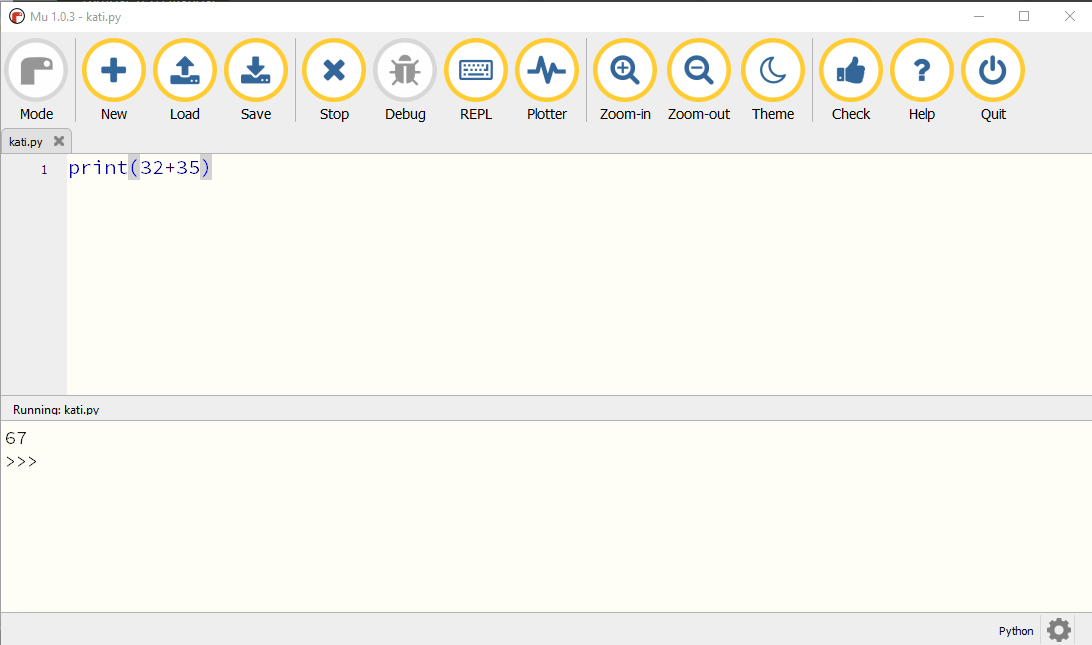
\includegraphics[width=\textwidth]{withprint.png}
\caption{Η εκτέλεση δίνει το αποτέλεσμα της πράξης}
\label{withprint}
\end{figure}
Μόλις έγραψες το πρώτο σου πρόγραμμα στην Python. Μάλιστα το πρόγραμμά σου κάνει κάτι. Υπολογίζει το αποτέλεσμα της πράξης $32+35$.
Μπορείς να αποθηκεύσεις το πρόγραμμά σου στον υπολογιστή σου κάνοντας κλικ στο εικονίδιο Save του Mu (εικόνα \ref{savewithmu}).
\begin{figure}
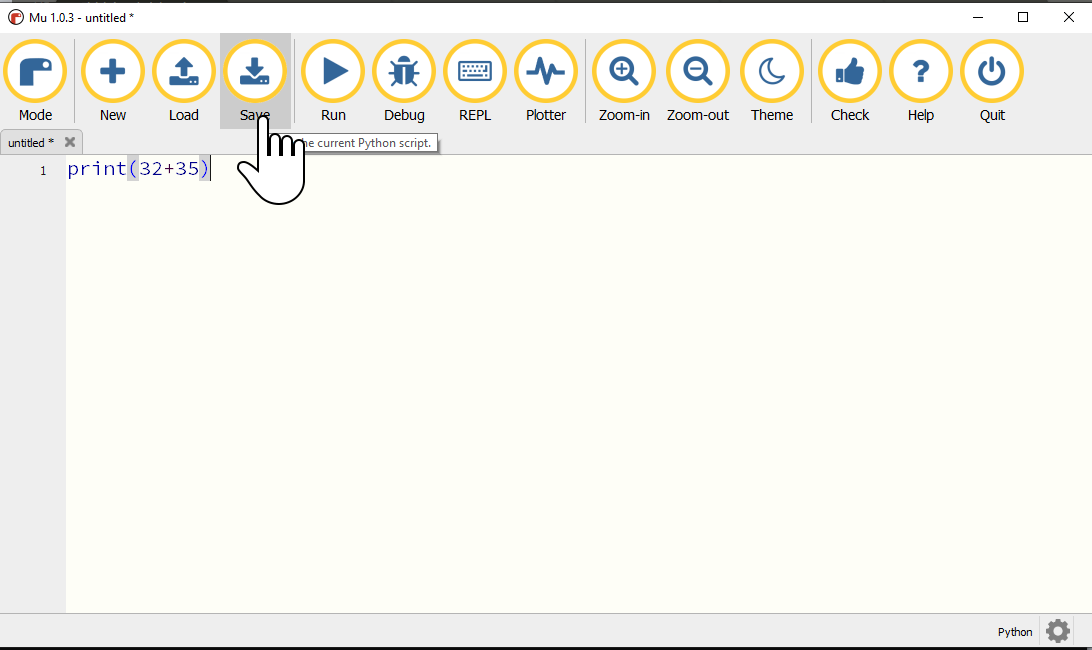
\includegraphics[width=\textwidth]{save.png}
\caption{Αποθήκευση με το Mu}
\label{savewithmu}
\end{figure}

\section{Απαρίθμηση}
Είδαμε ότι η Python μπορεί να κάνει πολύ γρήγορα, πολύπλοκες πράξεις ακόμη και με δυνάμεις, αλλά δεν είδαμε ακόμη τις απλές ασκήσεις που υπάρχουν στις πρώτες σελίδες του βιβλίου. Όπως για παράδειγμα ποιοι είναι οι τρεις προηγούμενοι αριθμοί του 289 και ποιο οι δύο επόμενοι \sel{13}. 

Σε ένα πρόγραμμα χρειαζόμαστε δεδομένα εισόδου και εξόδου, μπορούμε να γράψουμε ένα πρόγραμμα που ννα δέχεται σαν είσοδο τον βασικό αριθμό
και το πόσους αριθμούς πριν και μετά θα τυπώσουμε. Μέχρι να φτάσουμε εκεί μπορούμε να λύσουμε το πρόβλημα της σελίδας 13 με το παρακάτω πρόγραμμα:
\begin{lstlisting}
print(289-3)
print(289-2)
print(289-1)
print(289+1)
print(289+2)
\end{lstlisting}
που δίνει το αποτέλεσμα
\begin{lstlisting}
286
287
288
290
291
\end{lstlisting}

Πιο σωστό θα ήταν να τυπώσουμε κάποια μηνύματα ενδιάμεσα. Σε αυτή την περίπτωση θα γράψουμε τις παρακάτω εντολές.
\begin{lstlisting}
print("(@* Οι  προηγούμενοι αριθμοί είναι:*@)")
print(289-3)
print(289-2)
print(289-1)
print("(@* Οι επόμενοι αριθμοί είναι:*@)")
print(289+1)
print(289+2)
\end{lstlisting}

Για να εμφανίσει η print τις λέξεις που θέλουμε πρέπει να τις βάλουμε μέσα σε εισαγωγικά. Η Python υποστηρίζει είτε μονά εισαγωγικά, είτε διπλά. Αυτά εισάγονται συνήθως με το ίδιο κουμπί του πληκτρολογίου (κοντά στο ENTER), είτε με SHIFT ή χωρίς. Θυμήσου να κλείνεις τα εισαγωγικά με τον ίδιο τρόπο που τα άνοιξες. Στο πρόγραμμα Mu τα εισαγωγικά αυτά δεν φαίνονται όπως σε άλλα πρόγραμματα σαν `Εισαγωγικά' ή ``Εισαγωγικά " ή <<Εισαγωγικά>>, αλλά φαίνονται κάπως πιο απλά και ίδια στο άνοιγμα και το κλείσιμο \lstinline{'Εισαγωγικά'} ή  \lstinline{"Εισαγωγικά"}. 

Αν θέλουμε να αλλάξουμε το 289 και να βάλουμε έναν άλλο αριθμό,π.χ. το 132 θα πρέπει να αντικαταστήσουμε το 289 μέσα σε όλες τις εντολές print με το 132.
\begin{lstlisting}
print("(@*Οι  προηγούμενοι αριθμοί είναι:*@)")
print(132-3)
print(132-2)
print(132-1)
print("(@*Οι επόμενοι αριθμοί είναι:*@)")
print(132+1)
print(132+2)
\end{lstlisting}

Υπάρχει όμως ένας καλύτερος τρόπος, ο τρόπος αυτός είναι να δώσουμε ένα όνομα στον αριθμό μας. Μπορούμε να πούμε ότι το n είναι το όνομα του αριθμού. Αυτό γίνεται με την εντολή \lstinline{n=132}. Τότε το πρόγραμμά μας γίνεται:
\begin{lstlisting}
n = 132
print("(@*Οι  προηγούμενοι αριθμοί είναι:*@)")
print(n-3)
print(n-2)
print(n-1)
print("(@*Οι επόμενοι αριθμοί είναι:*@)")
print(n+1)
print(n+2)
\end{lstlisting}

Μετά την εντολή \lstinline{n=132} η Python ξέρει ότι το n είναι ένα όνομα για το 132 και μπορεί να κάνει πράξεις με αυτό. Για παράδειγμα n+1 κάνει τώρα 133.

Αν θέλουμε να κάνουμε τώρα το ίδιο πρόγραμμα αλλά όχι για το 132 αλλά για το 210, χρειάζεται να αλλάξουμε μόνο μία γραμμή και το πρόγραμμά μας να γίνει ως εξής:
\begin{lstlisting}
n = 210
print("(@*Οι  προηγούμενοι αριθμοί είναι:*@)")
print(n-3)
print(n-2)
print(n-1)
print("(@*Οι επόμενοι αριθμοί είναι:*@)")
print(n+1)
print(n+2)
\end{lstlisting}

Στην Python, όταν δίνουμε ένα όνομα σε έναν αριθμό (με τον τελεστή =) τότε δημιουργούμε μια μεταβλητή. Η μεταβλητή έχει ένα όνομα, στην περίπτωσή μας το n, και μια τιμή, στην περίπτωσή μας το 210.

Αν αντί για τους επόμενους δύο αριθμούς θέλαμε τους επόμενους \textbf{δέκα} θα γράφαμε ένα πρόγραμμα όπως το παρακάτω:
\begin{lstlisting}
n = 210
print(n)
print(n+1)
print(n+2)
print(n+3)
print(n+4)
print(n+5)
print(n+6)
print(n+7)
print(n+8)
print(n+9)
print(n+10)
\end{lstlisting}
Το παραπάνω πρόγραμμα εμφανίζει και τον αριθμό μας n, δηλαδή το 210.

Για να μην γράφουμε πολλές εντολές όταν κάνουμε το ίδιο πράγμα χρησιμοποιούμε την εντολή for.
Το πρόγραμμά μας με την for μπορεί να γίνει:
\begin{lstlisting}
n = 210
for i in 0,1,2,3,4,5,6,7,8,9,10:
    print(n+i)
\end{lstlisting}
Όταν γράψεις την for στην Python θα πρέπει να δηλώσεις ποιες εντολές θα εκτελεστούν πολλές φορές. Αυτή η δήλωση γίνεται βάζοντας αυτές τις εντολές λίγο πιο μέσα χρησιμοποιώντας το πλήκτρο κενό ή το πλήκτρο tab. Μια καλή πρακτική είναι να βάζεις τέσσερα κενά. Έτσι, πριν την εντολή \lstinline{print(n+i)} βάζεις τέσσερα κενά δηλαδή \lstinline[showspaces=true]{    print(n+i)}.
Το πρόγραμμα αυτό σημαίνει πως για το i μέσα στο σύνολο 0, 1, 2, 3, \ldots 10 και με αυτή τη σειρά εμφάνισε το n+i. Έτσι το αποτέλεσμα είναι το αναμενόμενο
\begin{lstlisting}
210
211
212
213
214
215
216
217
218
219
220
\end{lstlisting}


Στην Python υπάρχει ένας πιο εύκολος τρόπος να γράψουμε τους αριθμούς από το 0 έως το 10. Αυτός ο τρόπος είναι η εντολή range και συγκεκριμένα η range(11). Η range(11) φτιάχνει τους αριθμούς από το 0 μέχρι το 10 οι οποίοι είναι σε πλήθος 11. 
\begin{lstlisting}
>>> list(range(11))
[0,1,2,3,4,5,6,7,8,9,10]
\end{lstlisting}
Έτσι το πρόγραμμά μας γίνεται:
\begin{lstlisting}
n = 210
for i in range(11):
    print(n+i)
\end{lstlisting}

Οπότε μπορούμε να δώσουμε όνομα στο παραπάνω πρόγραμμα ως εξής:
\begin{lstlisting}
def meta(n,d):
    for i in range(d+1):
        print(n+i)
\end{lstlisting}
Θα έχουμε το παραπάνω αποτέλεσμα αν εκτελέσουμε το πρόγραμμα ως εξής:
\begin{lstlisting}
>>> meta(210,10)
\end{lstlisting}
Μπορούμε να γράψουμε το πρόγραμμα για τους αριθμούς πριν και μετά ως εξής:
\begin{lstlisting}
def prinmeta(n,d):
  for i in range(d,0,-1):
    print(n-i)
  for i in range(d+1):
    print(n+i)
\end{lstlisting}
Αν γράψουμε την παρακάτω εντολή:
\begin{lstlisting}
>>> prinmeta(210,10)
200
201
202
203
204
205
206
207
208
209
210
211
212
213
214
215
216
217
218
219
220
\end{lstlisting}
Με το πρόγραμμα αυτό μπορούμε να δοκιμάσουμε και το εξής:
\begin{lstlisting}
>>> prinmeta(283,3)
280
281
282
283
284
285
286
\end{lstlisting}



\section{Στρογγυλοποίηση}
Το βιβλίο των Μαθηματικών της Α' Γυμνασίου αναφέρει πως
Για να στρογγυλοποιήσουμε έναν φυσικό αριθμό \sel{12}:
\begin{enumerate}
  \item Προσδιορίζουμε την τάξη στην οποία θα γίνει η στρογγυλοποίηση
  \item Εξετάζουμε το ψηφίο της αμέσως μικρότερης τάξης
  \item Αν αυτό το ψηφίο είναι μικρότερο του 5 (δηλαδή 0, 1, 2, 3 ή 4) το ψηφίο αυτό και όλα τα ψηφία των υπόλοιπων τάξεων μηδενίζονται.
  \item Αν είναι μεγαλύτερο ή ίσο του 5 (δηλαδή 5, 6, 7, 8 ή 9) το ψηφίο αυτό και όλα τα ψηφία των υπόλοιπων τάξεων αντικαθίστανται από το 0 και το ψηφίο της τάξης στρογγυλοποίησης αυξάνεται κατά 1.
\end{enumerate}

Ας πούμε ότι θέλουμε να στρογγυλοποιήσουμε τον αριθμό 454.018.512 στα εκατομμύρια. Η απάντηση που περιμένουμε είναι 454 εκατομμύρια.
Για να τα καταφέρουμε θα χρησιμοποιήσουμε την διαίρεση. Όμως στην Python υπάρχουν \emph{δύο} διαιρέσεις μία με το σύμβολο / και μία με το σύμβολο //. Ας δούμε τις διαφορές τους στο REPL.
\begin{lstlisting}
>>> x = 454018512
>>> print(x/1000000)
454.018512
>>> print(x//1000000)
454
\end{lstlisting}
Η <<κανονική>> διαίρεση, με τη μία κάθετο /, δίνει το αποτέλεσμα της διαίρεσης με τα δεκαδικά ψηφία. Η <<ακέραια>> διαίρεση δίνει μόνο τον ακέραιο αριθμό. Δεν μπορούμε να πούμε ότι η ακέραια διαίρεση θα μας δώσει την στρογγυλοποίηση γιατί η ακέραια διαίρεση δεν στρογγυλοποιεί τα δεκαδικά ψηφία αλλά τα απορρίπτει εντελώς. Έτσι, ακόμη και αν είχαμε 454918512 κατοίκους η ακέραια διαίρεση θα δώσει 454 αντί για το στρογγυλοποιημένο που είναι 455.
\begin{lstlisting}
>>> x = 454918512
>>> print(x/1000000)
454.918512
>>> print(x//1000000)
454
\end{lstlisting}

Χρειάζεται επομένως να δούμε το ψηφίο της αμέσως χαμηλότερης τάξης το οποίο είναι το πρώτο δεκαδικό της κανονικής διαίρεσης. Για να το απομονώσουμε αφαιρούμε από το αποτέλεσμα της κανονικής διαίρεσης το ακέραιο μέρος.
\begin{lstlisting}
>>> x = 454018512
>>> x/1000000 - x//1000000
0.018511999999986983
\end{lstlisting}
Οπότε τώρα έχουμε δύο ενδεχόμενα αν το αποτέλεσμα αυτής της πράξης είναι μικρότερο από $0,5$, όπως παραπάνω, τότε το αποτέλεσμα που ψάχνουμε είναι το αποτέλεσμα της ακέραιας διαίρεσης. Αλλιώς πρέπει να προσθέσουμε τον αριθμό ένα στο αποτέλεσμα της ακέραιας διαίρεσης.
Αυτό γίνεται με την εντολή if, που σημαίνει στα αγγλικά αν. Για ευκολία μπορούμε να ονομάσουμε d την διαφορά των δύο διαιρέσεων με την εντολή:
\begin{lstlisting}
d = x/1000000 - x//1000000
\end{lstlisting}
Επειδή το πρόγραμμα γίνεται μεγαλύτερο τώρα θα το γράψουμε στο πάνω παράθυρο του Mu.
\begin{lstlisting}
x = 454018512
d = x/1000000 - x//1000000
if d < 0.5:
    print(x//1000000)
else:
    print(x//1000000 + 1)
\end{lstlisting}
Την \lstinline{if} την γράφουμε ως εξής:
\begin{lstlisting}
if (@*συνθήκη*@):
    (@*εντολές που εκτελούνται*@)
    (@*αν ισχύει η συνθήκη*@)
else:
    (@*εντολές που εκτελούνται*@)
    (@*αν δεν ισχύει η συνθήκη*@)
\end{lstlisting}
Θυμήσου να βάζεις την άνω κάτω τελεία (:) μετά τη συνθήκη και μετά τη λέξη else.

Αν στο ίδιο πρόγραμμα και βάλεις αντί για 454.018.512 τον αριθμό 454.918.512 θα δεις ότι θα εμφανιστεί το σωστό αποτέλεσμα (455).

Αν θέλεις στρογγυλοποίηση στις χιλιάδες τότε το πρόγραμμά σου γίνεται:
\begin{lstlisting}
x = 454018512
d = x/1000 - x//1000
if d < 0.5:
    print(x//1000)
else:
    print(x//1000 + 1)
\end{lstlisting}
και το αποτέλεσμα είναι 454019.

\begin{exercise}
Για να γίνει το 454.018.512, 450 εκατομμύρια \sel{12} η στρογγυλοποίηση γίνεται στις δεκάδες των εκατομμυρίων. Μπορείς να γράψεις ένα πρόγραμμα που να στρογγυλοποιεί αριθμούς στις δεκάδες των εκατομμυρίων;
\end{exercise}
Η απάντηση με βάση το παραπάνω πρόγραμμα είναι η εξής:
\begin{lstlisting}
x = 454018512
d = x/10000000 - x//10000000
if d < 0.5:
    print(x//10000000*10)
else:
    print((x//10000000 + 1)*10)
\end{lstlisting}
Σε αυτή την περίπτωση από τον αριθμό 454.018.512,00 πρέπει να φτάσουμε πρώτα στις δεκάδες των εκατομμυρίων και μετά πολλαπλασίαζουμε με το δέκα ώστε να μην απαντήσει το πρόγραμμα 45 (δεκάδες εκατομμύρια) αλλά 450 (εκατομμύρια).

\section{Επανάληψη στις πράξεις}
\begin{exercise}
Συμπλήρωσε τον πίνακα τα τετράγωνα και τους κύβους των αριθμών από το 8 μέχρι το 25 \sel{22}.
\end{exercise}
\begin{lstlisting}
for a in range(8,26):
    print(a**2,end =" ")
print()
print()
for a in range(8,26):
    print(a**3,end=" ")
\end{lstlisting}
Το αποτέλεσμα αυτού του προγράμματος είναι:

\begin{lstlisting}
64 81 100 121 144 169 196 225 256 289 324 361 400 441 484 529 576 625 

512 729 1000 1331 1728 2197 2744 3375 4096 4913 5832 6859 8000 9261 
10648 12167 13824 15625
\end{lstlisting}

Η εντολή print μπορεί να πάρει περισσότερα από ένα ορίσματα, το πρώτο όρισμα είναι αυτό που θα εμφανίσει. Το δεύτερο όρισμα που δώσαμε είναι το end και το ορίσαμε ίσο με το κενό (\lstinline{end=" "}) που σημαίνει ότι η print όταν εμφανίσει το πρώτο όρισμα δεν θα αλλάξει γραμμή αλλά θα αφήσει ένα κενό. Η εντολή print() αλλάζει απλά γραμμή.
\begin{exercise}
Βρες τα τετράγωνα των αριθμών 10,20,30,40,50,60,70,80 και 90 \sel{22}.
\end{exercise}
Το πρόγραμμα είναι το εξής:
\begin{lstlisting}
for i in range(10,100,10):
    print(i**2,end=',')
\end{lstlisting}
και το αποτέλεσμα της εκτέλεσης του προγράμματος είναι
\begin{lstlisting}
100,400,900,1600,2500,3600,4900,6400,8100,
\end{lstlisting}

\begin{exercise}
Βρες τους κύβους των αριθμών 10,20,30,40,50
\end{exercise}

\begin{lstlisting}
for i in range(10,60,10):
    print(i**3,end=', ')  
\end{lstlisting}
Το αποτέλεσμα της εκτέλεσης είναι:
\begin{lstlisting}
1000, 8000, 27000, 64000, 125000, 
\end{lstlisting}

\section{Ανάπτυγμα}
\begin{exercise}\sel{21}Να γραφεί το ανάπτυγμα του αριθμόύ 7.604 με χρήση των δυνάμεων του 10.
\end{exercise}
Η απάντηση είναι $7\cdot 10^3 + 6\cdot 10^2 + 0\cdot 10^1 + 4$.  Με συμβολισμό της Python η απάντηση που περιμένουμε είναι:
\begin{lstlisting}
7*10**3+6*10**2+0*10+4
\end{lstlisting}


%Το ανάπτυγμα του αριθμού σχετίζεται με τον τρόπο με τον οποίο διαβάζεις τους αριθμούς. Μόλις δεις το 7.604 ή 7604 όπως είναι στην Python αμέσως διαβάζεις εφτά χιλιάδες εξιακόσια τέσσερα. Αν όμως ο αριθμός ήταν ο 7102234 ίσως χρειαζόσουν λίγο περισσότερο χρόνο και κάποια βήματα για να τον διαβάσεις. Ας δούμε αυτά τα βήματα. Πρώτα θα χώριζες σε τριάδες από το τελευταίο προς το πρώτο για να βρεις το 7.103.234 ύστερα θα έβρισκες ότι το 7 αναφέρεται σε εκατομμύρια και τέλος θα διάβαζες όλον τον αριθμό σε 7 εκατομμύρια εκατόν τρεις χιλιάδες διακόσια τριάντα τέσσερα.

Ας υποθέσουμε ότι ξέρουμε ότι ο αριθμός είναι τετραψήφιος, πως μπορούμε να βρούμε το ανάπτυγμα του. Ξεκινάμε από το πρώτο ψηφίο. Ποιο είναι το πρώτο ψηφίο; Το πρώτο ψηφίο προκύπτει αν διαιρέσουμε τον αριθμό με το 1000 και κρατήσουμε το ακέραιο μέρος.
Δοκίμασε στο REPL:
\begin{lstlisting}
>>> 7604//1000
7
\end{lstlisting}
Βρήκες το πρώτο ψηφίο, πώς μπορείς να βρεις το δεύτερο; Ας διαιρέσουμε με το 100.
\begin{lstlisting}
>>> 7604//100
76
\end{lstlisting}
Στην ουσία δεν μπορείς να διαιρέσεις τον αρχικό αριθμό με το 100 αλλά αυτόν που σου μένει αφού αφαιρέσεις το πρώτο ψηφίο που έχεις ήδη βρει δηλαδή το 604.
\begin{lstlisting}
>>> 604//100
6
\end{lstlisting}

Τα σωστά βήματα είναι:
\begin{enumerate}
    \item Διαιρείς τον αριθμό με το 1000 και κρατάς το ακέραιο μέρος 
    \item Αφαιρείς από τον αριθμό τις χιλιάδες που βρήκες
    \item Διαιρείς τον αριθμό με το 100 και κρατάς το ακέραιο μέρος
    \item Αφαιρείς από τον αριθμό τις εκατοντάδες που βρήκες
    \item Διαιρείς τον αριθμό με το 10 και κρατάς το ακέραιο μέρος
    \item Αφαιρείς από τον αριθμό τις δεκάδες που βρήκες
    \item Σου μένουν οι μονάδες
\end{enumerate}
Ας ονομάσουμε τον αριθμό 7604, n (\lstinline{n=7604}), και το πρώτο ψηφίο, στην περίπτωσή μας τις χιλιάδες, prwto.
\begin{lstlisting}
>>> n = 7604
>>> prwto = n//1000
>>> prwto
7
>>> n = n - prwto*1000
>>> n
604
\end{lstlisting}

Ας δούμε λίγο αυτή την εντολή:
\begin{lstlisting}
n = n - prwto*1000
\end{lstlisting}
Θυμήσου ότι εκείνη τη στιγμή το n έχει την τιμή 7604 και το prwto την τιμή 7. Η παραπάνω εντολή σημαίνει:
\begin{enumerate}
    \item Κάνε τις πράξεις που υπάρχουν δεξιά από το σύμβολο ίσον
    \item Δώσε σαν τιμή στην μεταβλητή που υπάρχει αριστερά από το σύμβολο ίσον το αποτέλεσμα των πράξεων
\end{enumerate}
Έτσι η Python κάνει πρώτο \lstinline{n-prwto*1000} δηλαδή $7604-7*1000 = 604$ και αυτό το αποτέλεσμα το δίνει σαν τιμή στην μεταβλητή που υπάρχει αριστερά από το = δηλαδή στη μεταβλητή n. Έτσι το n τώρα είναι 604. \emph{Προσοχή!} Η τιμή 7604 δεν υπάρχει στην μεταβλητή n. Με αυτόν τον τρόπο το n έχει πάντα τον αριθμό που χρειάζεσαι για να απομονώσεις το επόμενο ψηφίο του αριθμού.

Έτσι ένα συνολικό πρόγραμμα που μπορείς να γράψεις είναι:
\begin{lstlisting}
n = 7604
prwto = n//1000
n = n - prwto*1000
deutero = n//100
n = n - deutero*100
trito = n //10
n = n - trito*10
tetarto = n
print(prwto,end='')
print('*10**3+',end='')
print(deutero,end='')
print('*10**2+',end='')
print(trito,end='')
print('*10+',end='')
print(tetarto)
\end{lstlisting}
Όταν το εκτελέσεις δίνει το σωστό αποτέλεσμα:
\begin{lstlisting}
7*10**3+6*10**2+0*10+4
\end{lstlisting}

Το παραπάνω πρόγραμμα δουλεύει με όλους τους τετραψήφιους αριθμούς, απλά άλλαξε το n σε όποιον αριθμό θέλεις στην αρχή του προγράμματος.


Όμως οι 7 εντολές print δεν είναι ο καλύτερος τρόπος να γράψεις το αποτέλεσμα. Θα ήταν καλύτερα να τυπώσουμε αυτά που πρέπει για κάθε ψηφίο χωριστά ώστε να έχουμε τέσσερις εντολές print ως εξής:
\begin{lstlisting}
n = 7604
prwto = n//1000
n = n - prwto*1000
deutero = n//100
n = n - deutero*100
trito = n //10
n = n - trito*10
tetarto = n
print(prwto + '*10**3+',end='')
print(deutero + '*10**2+',end='')
print(trito + '*10+',end='')
print(tetarto)
\end{lstlisting}

Εξάλλου όταν έχουμε πρόσθεση με λέξεις η Python τις βάζει δίπλα δίπλα οπότε για το \lstinline{print(prwto + '*10**3+',end='')}
θα περιμέναμε να εμφανιστεί το \lstinline{7*10**3+}. 
Άν όμως εκτελέσεις το παραπάνω πρόγραμμα θα προκύψει ένα μήνυμα λάθους.
\begin{lstlisting}
Traceback (most recent call last):
  File "a.py", line 9, in <module>
    print(prwto + '*10**3+',end='')
TypeError: unsupported operand type(s) for +: 'int' and 'str'
\end{lstlisting}
Αν προσέξουμε λίγο θα δούμε ότι το λάθος αφορά την ένατη γραμμή (line 9) και το λάθος είναι TypeError: unsupported operand type(s) for +: 'int' and 'str'.
Σε μετάφραση από τα αγγλικά το μήνυμα λάθους γράφει:

ΛάθοςΤύπων: μη υποστηριζόμενοι τύποι για το +: 'int' και 'str'

Τι είναι οι τύποι και προκύπτουν λάθη από αυτούς;

Οτιδήποτε χρησιμοποιούμε στην Python έχει τύπο. Μάλιστα μπορούμε να δούμε τον τύπο αυτό με την εντολή type. Έτσι δοκίμασε:
\begin{lstlisting}
>>> type(7)
<class 'int'>
>>> type('a')
<class 'str'>
>>> type('7')
<class 'str'>
\end{lstlisting} 

Βλέπουμε ότι οι αριθμοί έχουν τύπο `int', θα αγνοήσουμε τη λέξη class προς το παρόν. Ενώ οι λέξεις που έχουν τα εισαγωγικά έχουν τύπο `str'. Το `int' προκύπτει από την αγγλική λέξη `integer' που σημαίνει ακέραιος, και το `str' προκύπτει από την αγγλική λέξη `string' που σημαίνει μια σειρά από γράμματα και αριθμούς. Στα ελληνικά το `string' το μεταφράζουμε ως αλφαριθμητικό.

Το πρόβλημα είναι ότι η Python δεν μπορεί να προσθέσει έναν ακέραιο με ένα αλφαριθμητικό. Γι' αυτό δίνει και το μήνυμα λάθους. Ωστόσο, αυτό το πρόβλημα έχει λύση και είναι η μετατροπή του αριθμού σε αλφαριθμητικό με την εντολή str().
Δοκίμασε:
\begin{lstlisting}
>>> type(7)
<class 'int'>
>>> str(7)
'7'
>>> type('7')
<class 'str'>
\end{lstlisting} 

Το παραπάνω πρόγραμμα γίνεται λοιπόν:
\begin{lstlisting}
n = 7604
prwto = n//1000
n = n - prwto*1000
deutero = n//100
n = n - deutero*100
trito = n //10
n = n - trito*10
tetarto = n
print(str(prwto) + '*10**3+',end='')
print(str(deutero) + '*10**2+',end='')
print(str(trito) + '*10+',end='')
print(str(tetarto))
\end{lstlisting}

Που και πάλι δίνει τη σωστή απάντηση.

Μπορούμε να βάλουμε τα στοιχεία prwto, deutero, trito και tetarto σε μια λίστα που θα την ονομάσουμε psifia και θα έχει τέσσερα στοιχεία. Στην αρχή θα αρχικοποιήσουμε τη λίστα με κάποια τιμή ειδικά στην περίπτωση που ξέρουμε πόσο μεγάλη θα είναι όπως τώρα.

\begin{lstlisting}
n = 7604
psifia  = [0,0,0,0]
psifia[0] = n//1000
n = n - psifia[0]*1000
psifia[1] = n//100
n = n - psifia[1]*100
psifia[2] = n //10
n = n - psifia[2]*10
psifia[3] = n
print(str(psifia[0]) + '*10**3+',end='')
print(str(psifia[1]) + '*10**2+',end='')
print(str(psifia[2]) + '*10+',end='')
print(str(psifia[3]))
\end{lstlisting}
Όπως βλέπεις το πρώτο ψηφίο είναι το psifia[0], το δεύτερο ψηφίο είναι το psifio[1] κ.λ.π., οι πίνακες στην Python ξεκινάν από το 0.

Φαίνεται ότι κάνουμε τα ίδια πράγματα τρεις φορές όπως βλέπεις εδώ:
\begin{lstlisting}
psifia[0] = n//1000
n = n - psifia[0]*1000
psifia[1] = n//100
n = n - psifia[1]*100
psifia[2] = n //10
n = n - psifia[2]*10
\end{lstlisting}

Θα προσπαθήσουμε να τα κάνουμε με for όπου το i θα μετράει 0,1,2 έτσι το psifia[0] θα γίνει psifia[i]. Όμως θα πρέπει να υπολογίσουμε το 1000 το 1000 είναι 10**3 και στην επόμενη επανάληψη είναι 10**2 κ.ο.κ. οπότε είναι 10**(3-i).
Άρα οι τρεις παραπάνω εντολές μπορούν να αντικατασταθούν με μία for
\begin{lstlisting}
for i in range(3):
    psifia[i] = n//10**(3-i)
    n = n - psifia[i]* 10**(3-i)
\end{lstlisting}

Το ίδιο πρέπει να γίνει και με τις τρεις εντολές print:
\begin{lstlisting}
print(str(psifia[0]) + '*10**3+',end='')
print(str(psifia[1]) + '*10**2+',end='')
print(str(psifia[2]) + '*10+',end='')
\end{lstlisting}
Θα πρέπει να κάνουμε έναν ιδιαίτερο χειρισμό για τις δυνάμεις όπου θα πρέπει να μειώνονται καθώς συνέχίζουν οι επαναλήψεις οπότε αντί για `*10**3΄ χρειαζόμαστε `*10**(3-i)+' όμως το 3-i είναι αριθμός οπότε για να το γράψουμε στην Python θα χρειαστεί να βάλουμε το str() και να γίνει \lstinline{'*10**'+str(3-i)+'+'}. Οι παραπάνω τρεις εντολές μπορούν τώρα να γραφούν με μία for ως εξής:
\begin{lstlisting}
for i in range(3):
    print(str(psifia[i]) + '*10**' + str(3-i) + '+',end='')
\end{lstlisting}
και όλο το πρόγραμμα να γίνει:
\begin{lstlisting}
n = 7604
psifia  = [0,0,0,0]
for i in range(3):
    psifia[i] = n//10**(3-i)
    n = n - psifia[i]* 10**(3-i)
psifia[3] = n
for i in range(3):
    print(str(psifia[i]) + '*10**' + str(3-i) + '+',end='')
print(str(psifia[3]))
\end{lstlisting}

Πώς μπορεί το πρόγραμμα αυτό να δουλεύει για όλους τους ακέραιους ανεξάρτητα από το μέγεθός τους; Αν μετατρέψουμε τον ακέραιο σε αλφαριθμητικό η Python μπορεί να μας πει πόσο μεγάλος είναι με την εντολή len, που είναι το μήκος του αλφαριθμητικού.
\begin{lstlisting}
>>> n = 7604
>>> len(str(n))
4
>>> n = 7102234
>>> len(str(n))
7
\end{lstlisting}

Και η αρχικοποίηση του πίνακα μπορεί να γίνει για όσα ψηφία θέλουμε (plithos) με την εντολή \lstinline{[0]*plithos}:
\begin{lstlisting}
>>> plithos = 7
psifia = [0] * plithos
>>> psifia
[0, 0, 0, 0, 0, 0, 0]
\end{lstlisting}

Αν υπολογίσουμε το plithos των ψηφίων με το len(str(n)) θα προκύψει 4, ωστόσο εμείς στο πρόγραμμά μας κάνουμε επαναλήψεις τρεις φορές γιατί χρειαζόμαστε ειδικό χειρισμό στο τελευταίο ψηφίο. Έτσι αντικαθιστούμε το 3 με plithos-1 παντού στο πρόγραμμα.
\begin{lstlisting}
n = 7604
plithos = len(str(n))
psifia  = [0]*plithos
for i in range(plithos-1):
    psifia[i] = n//10**(plithos-1-i)
    n = n - psifia[i]* 10**(plithos-1-i)
psifia[plithos-1] = n
for i in range(plithos-1):
    print(str(psifia[i]) + '*10**' + str(plithos-1-i) + '+',end='')
print(str(psifia[plithos-1]))
\end{lstlisting}

Μπορούμε να το γράψουμε με τη μορφή συνάρτησης ως εξής:
\begin{lstlisting}
def anaptygma(n):
  plithos = len(str(n))
  psifia  = [0]*plithos
  for i in range(plithos-1):
      psifia[i] = n//10**(plithos-1-i)
      n = n - psifia[i]* 10**(plithos-1-i)
  psifia[plithos-1] = n
  for i in range(plithos-1):
      print(str(psifia[i]) + '*10**' + str(plithos-1-i) + '+',end='')
  print(str(psifia[plithos-1]))

>>> anaptygma(7604)
7*10**3+6*10**2+0*10**1+4*10**0
>>> anaptygma(7102234)
7*10**6+1*10**5+0*10**4+2*10**3+2*10**2+3*10**1+4
\end{lstlisting}
Η Python έχει διάφορους τρόπους να συμπυκνώνει μεγάλα προγράμματα ακόμη και σε μία γραμμή. Ένας τέτοιος τρόπος να γραφτεί το ανάπτυγμα είναι ο εξής:
\begin{lstlisting}
>>> n = 7604
>>> '+'.join([x+'*10**'+str(len(str(n))-1-i) 
for (i,x) in enumerate(list(str(n)))])

'7*10**3+6*10**2+0*10**1+4*10**0'
\end{lstlisting}

\section{Ιστορικό σημείωμα}
\sel{17}

Όταν ο δάσκαλος ζήτησε από τους υπόλοιπους μαθητές να υπολογίσουν το άθροισμα $1+2+3+\ldots+98+99+100$, πριν οι υπόλοιποι αρχίσουν τις πράξεις ο μικρόος Γκάους το είχε ήδη υπολογίσει. Ο δάσκαλος ρώτησε έκπληκτος πώς το βρήκε. Τότε εκείνος έγραψε στον πίνακα:
O Γκάους σκέφτηκε πως το άθροισμα 
$$
1    +    2 + 3  + \ldots + 99 + 100
$$
είναι ίδιο με το
$$
100+  99+ 98+ \ldots +    2  + 1
$$
και αν αθροίσουμε τον πρώτο όρο με τον πρώτο όρο, τον δεύτερο με τον δεύτερο κ.ο.κ. Συνολικά αυτό γίνεται:
\begin{eqnarray}
\underbrace{(1+100) + (2+99) + \ldots  (99+2)+(100+1) }_{50 \text{φορές}} &=\\
101\cdot 100&\\
\end{eqnarray}

Άρα το άθροισμα $1 + 2 + 3+ \ldots + 99 + 100$ είναι $\frac{1}{2}101\times 100 = 5050$ .

Μπορείς να υπολογίσεις το άθροισμα $1 + 2 + 3+ \ldots + 999 + 1000$ με τον τρόπο του Γκάους;

Ας δούμε το πρόβλημα από την πλευρά της Python.
Μπορούμε να εμφανίζουμε τους αριθμούς από το 1 έως το 100 με το παρακάτω πρόγραμμα:
\begin{lstlisting}
for i in range(101):
    print(i)
\end{lstlisting}
Πώς όμως θα αθροίσουμε τους αριθμούς αυτούς. Θα φτάξουμε μιά νέα μεταβλητή athroisma και σε αυτή θα προσθέτουμε το i κάθε φορά. Το πρόγραμμα γίνεται:

\begin{lstlisting}
athroisma = 0
for i in range(101):
    athroisma = athroisma + i
print(athroisma)
\end{lstlisting}

Όμως επειδή το άθροισμα είναι χρήσιμο σε πολλές περιπτώσεις η Python έχει έτοιμο το άθροισμα με την εντολή sum. Δοκίμασε:
\begin{lstlisting}
>>> sum([1,2,3])
6
\end{lstlisting}

Με τον ίδιο τρόπο μπορείς να βρεις το άθροισμα $1 + 2 + 3+ \ldots + 99 + 100$:
\begin{lstlisting}
>>> sum(range(101))
5050
\end{lstlisting}

Τέλος ο τρόπος του μικρού Γκάους είναι:
\begin{lstlisting}
>>> 101*100/2
5050
\end{lstlisting}

Με την Python μπορούμε να υπολογίσουμε το άθροισμα από το 1 έως το 1000 και με τους δύο τρόπους:
\begin{lstlisting}
>>> sum(range(1001))
500500
>>> 1000*1001/2
500500.0
\end{lstlisting}
Στην Python to 500500.0 σημαίνει πως το δεκαδικό μέρος είναι 0 οπότε το αποτέλεσμα είναι και πάλι 500500.



%\chapter{Τι θα χρησιμοποιήσουμε;}
\section{Η γλώσσα προγραμματισμού Python}
Σε αυτές τις σημειώσεις θα χρησιμοποιήσουμε τη γλώσσα προγραμματισμού Python και μάλιστα την έκδοση 3. Υπάρχει και Python 2 αλλά υπάρχουν σχέδια για την αντικατάστασή της από την Python 3. Για να εγκαταστήσεις την Python 3 θα πρέπει να την κατεβάσεις από το επίσημο site της Python \href{https://www.python.org/}{www.python.org}. Κατεβάστε την πιο πρόσφατη έκδοση που σας προτείνει θα είναι κάτι σαν 3.8.2 ή κάτι 

\section{Ο επεξεργαστής προγραμμάτων Mu}
Μπορείς να γράψεις Python σε οποιοδήποτε πρόγραμμα υποστηρίζει απλό κείμενο, ακόμη και στο Σημειωματάριο, όμως σε αυτές τις σημειώσεις χρησιμοποιούμε τον επεξεργαστή Python, Mu Editor ή πιο απλά Mu που μπορείς να τον κατεβάσεις από τη σελίδα \href{https://codewith.mu/}{codewith.mu}. Μόλις το ανοίξεις θα δεις την εικόνα \ref{Mu}. 
\begin{figure}
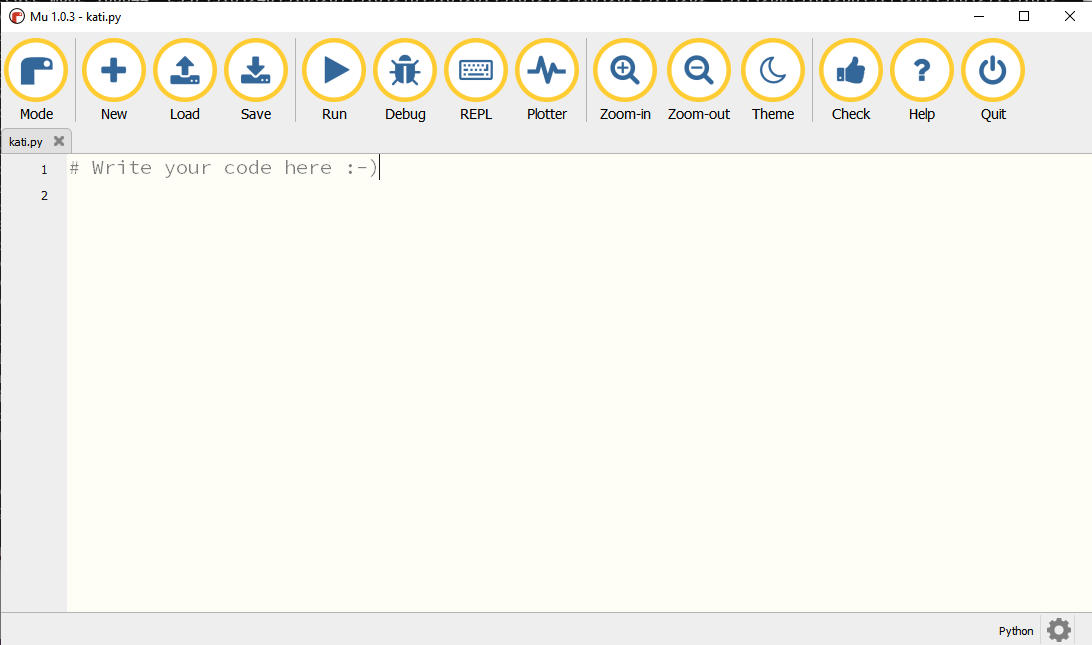
\includegraphics[width=\textwidth]{mu.png}
\label{Mu}
\caption{Mu: Ένας επεξεργαστής προγραμμάτων Python}
\end{figure}

Μπορείς να πατήσεις την εκτέλεση (κουμπί Run) και τότε θα δεις ότι το παράθυρο χωρίζεται σε δύο τμήματα (Εικόνα \ref{Mu2}).  Αν θες να δοκιμάσεις ένα ολόκληρο πρόγραμμα μπορείς να το πληκτρολογήσεις στο βασικό παράθυρο (τώρα γράφει `\#Write your code here`). Ενώ αν θες να δοκιμάσεις κάποια εντολή τότε μπορείς να την πληκτρολογήσεις στο κάτω παράθυρο (τώρα γράφει $>>>$).  Το κάτω παράθυρο ονομάζεται REPL, από τα αρχικά των λέξεων Read, Eval, Print, Loop δηλαδή Διάβασε, Εκτέλεσε (την εντολή/έκφραση), Τύπωσε, Επανάλαβε. Το REPL θα διαβάσει την εντολή, θα την εκτελέσει και θα μας δώσει το αποτέλεσμα.

Από εδώ και πέρα όταν βλέπετε στις σημειώσεις τα τρία σύμβολα ``μεγαλύτερο από'' ($>>>$) θα πληκτρολογείτε τις αντίστοιχες εντολές στο κάτω παράθυρο (REPL). Τα μεγαλύτερα προγράμματα που δεν θα έχουν αυτό το σύμβολο θα τα πληκτρολογείτε στο πάνω παράθυρο.

\fbox{
	\parbox{0.8\textwidth}{%
	\textbf{Συμβουλή:} Αν χρησιμοποιείτε την ηλεκτρονική έκδοση αυτών των σημειώσεων, θυμηθείτε να πληκτρολογείτε τις εντολές και να μην τις κάνετε αντιγραφή επικόλληση.
	}
}


Στην αρχή θα δοκιμάσεις κάποια πράγματα στο κάτω παράθυρο, όμως μην ανησυχείς σύντομα θα γράφεις τα δικά σου προγράμματα στο πάνω παράθυρο.

\begin{figure}
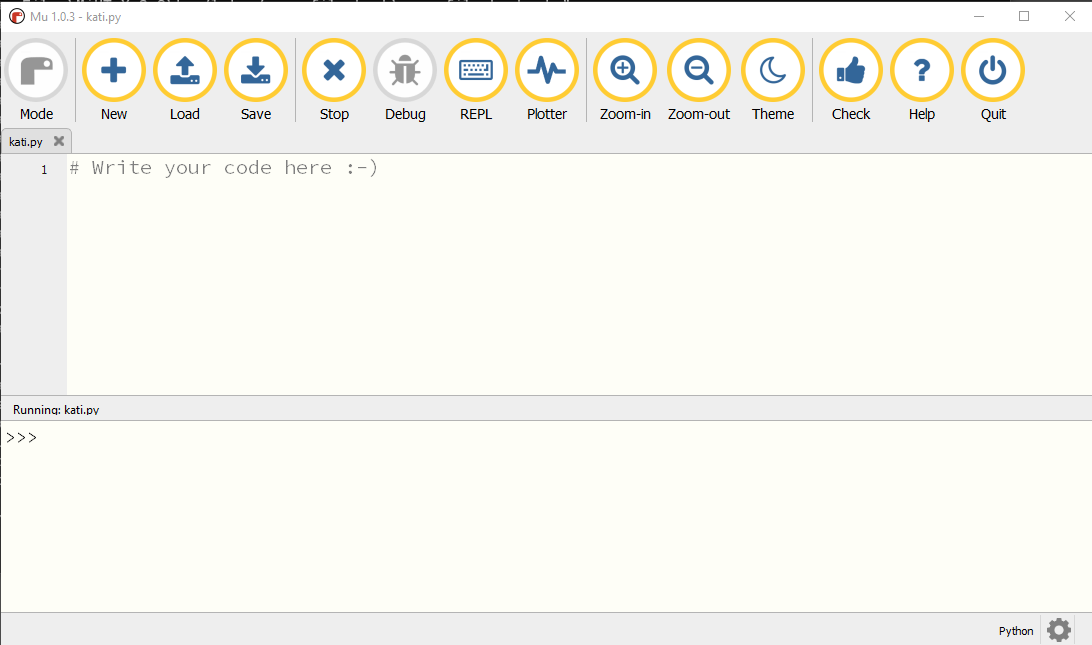
\includegraphics[width=\textwidth]{mu2.png}
\label{Mu2}
\caption{Το πρόγραμμα Mu όταν εκτελείτε ένας κώδικας}
\end{figure}

\section{Το βιβλίο μαθηματικών της Α΄ Γυμνασίου}
Σε αυτές τις σημειώσεις οι περισσότερες ασκήσεις είναι από το βιβλίο Μαθηματικών της Α΄ Γυμνασίου των Βανδουλάκη, Καλλιγά, Μαρκάκη και Φερεντίνου (Εικόνα \ref{matha}).

\begin{figure}
\centering

\includegraphics[width=0.8\textwidth]{matha.jpg}
\label{matha}
\caption{Το εξώφυλλο του βιβλίου των Μαθηματικών που θα χρησιμοποιήσουμε}
\end{figure}
%\chapter{Φυσικοί αριθμοί}

\section{Οι αριθμοί και η Python}

Οι φυσικοί αριθμοί είναι οι αριθμοί από 0, 1, 2, 3, 4, 5, 6, \ldots, 98, 99, 100, \ldots, 1999, 2000, 2001, \ldots

Η Python μπορεί να χειριστεί φυσικούς αριθμούς. Δοκιμάστε να γράψετε στο REPL έναν φυσικό αριθμό, θα δείτε ότι η Python θα τον επαναλάβει. Π.χ. δείτε τον αριθμό εκατόν είκοσι τρια (123).
\begin{lstlisting}
>>> 123
123
\end{lstlisting}

Στην Python όμως θα πρέπει να ακολουθείς κάποιους επιπλέον κανόνες. Για παράδειγμα στους αριθμούς δεν πρέπει να βάζεις τελείες στις χιλιάδες όπως στο χαρτί. Αν το κάνεις στην καλύτερη περίπτωση θα προκύψει κάποιο λάθος, στην χειρότερη ο υπολογιστής θα καταλάβει διαφορετικό αριθμό από αυτόν που εννοείς.
Δείτε το παρακάτω παράδειγμα στο REPL.
\begin{lstlisting}
>>> 1.000.000
  File "<stdin>", line 1
    1.000.000
            ^
SyntaxError: invalid syntax
>>> 100.000
100.0
\end{lstlisting}
Σε αυτό το παράδειγμα, η Python δεν καταλαβαίνει καθόλου τον αριθμό 1.000.000 γραμμένο με τελείες ενώ μεταφράζει το 100.000 σε 100.0, που για την Python σημαίνει 100 (εκατό). Γι' αυτόν τον λόγο δεν βάζουμε καθόλου τελείες έτσι αν θέλουμε να γράψουμε το ένα εκατομμύριο θα γράψουμε 1000000.
\begin{lstlisting}
>>> 1000000
1000000
\end{lstlisting}

\section{Πρόσθεση, αφαίρεση και πολλαπλασιασμός φυσικών αριθμών}
Μια γλώσσα προγραμματισμού μπορεί να εκτελέσει απλές πράξεις πολύ εύκολα. Στο βιβλίο των μαθηματικών  σου μπορείς να βρεις πολλές ασκήσεις με πράξεις. Μπορείς να τις λύσεις με την Python.

\begin{exercise}
\sel{16}
Να υπολογιστούν τα γινόμενα: 

(α) $35 \cdot 10$, 

(β) $421 \cdot 100$,

(γ) $5 \cdot 1.000$,

(δ) $27 \cdot 10.000$
\end{exercise}

Η python μπορεί να κάνει αυτές τις πράξεις ως εξής:
\begin{lstlisting}
>>> 35*10
350
>>> 421*100
42100
>>> 5*1000
5000
>>> 27*10000
270000
\end{lstlisting}

Ο τελεστής του πολλαπλασιασμού είναι το αστεράκι * (SHIFT+8) στο πληκτρολόγιο. Εναλλακτικά, μπορείτε να το βρείτε στο αριθμητικό πληκτρολόγιο. 

\begin{exercise}
\sel{16}
Να εκτελεστούν οι ακόλουθες πράξεις:

(α) $89\cdot 7 + 89\cdot 3$

(β) $23 \cdot 49 + 77 \cdot 49$

(γ) $76 \cdot 13 – 76 \cdot 3$

(δ) $284 \cdot 99$
\end{exercise}
\begin{lstlisting}
>>> 89*7+89*3
890
>>> 23*49+77*49
4900
>>> 76*13-76*3
760
>>> 284*99
28116
\end{lstlisting}

Στις παραπάνω περιπτώσεις η python εκτελεί πρώτα τους πολλαπλασιασμούς και μετά τις προσθέσεις/αφαιρέσεις δίνοντας έτσι το αποτέλεσμα που αναμένεται. Για παράδειγμα 89\*7 + 89\*3 = 623 + 267 = 890, που είναι το σωστό αποτέλεσμα.

\begin{exercise}
\sel{18}
Υπολογίστε:

(α)  $157 + 33$ 

(β)  $122 + 25 + 78$

(γ)  $785 - 323$

(δ)  $7.321 - 4.595$

(ε)  $60 - (18 - 2)$

(στ) $52 - 11 -9$

(ζ)  $23 \cdot 10$

(η)  $97 \cdot 100$

(θ)  $879 \cdot 1.000$
\end{exercise}
Σε python τα παραπάνω υπολογίζονται ως εξής:
\begin{lstlisting}
>>> 157+33
190
>>> 122+25+78
225
>>> 785-323
462
>>> 7321-4595
2726
>>> 60-(18-2)
44
>>> 52-11-9
32
>>> 23*10
230
>>> 97*100
9700
>>> 879*1000
879000
\end{lstlisting}
Οι παρενθέσεις (SHIFT+9 και SHIFT+0) αλλάζουν τη σειρά των πράξεων. Οι πράξεις που είναι μέσα στην παρένθεση εκτελούνται πρώτες. Γι' αυτό το λόγο 60-(18-2)=60-16=44.

\begin{exercise}
\sel{18}
Σε ένα αρτοποιείο έφτιαξαν μία μέρα 120 κιλά άσπρο ψωμί, 135 κιλά χωριάτικο, 25 κιλά σικάλεως και 38 κιλά πολύσπορο. Πουλήθηκαν 107 κιλά άσπρο ψωμί, 112 κιλά χωριάτικο, 19 κιλά σικάλεως και 23 κιλά πολύσπορο. Πόσα κιλά ψωμί έμειναν απούλητα;
\end{exercise}
Με τις γνώσεις που έχουμε θα πρέπει να μετατρέψουμε το παραπάνω πρόβλημα σε μια αριθμητική παράσταση ώστε η python να μπορεί να την υπολογίσει, στη συγκεκριμένη περίπτωση η σωστή παράσταση είναι $$(120-107)+(135-112)+(25-19)+(38-23)$$
\begin{lstlisting}
>>> (120-107)+(135-112)+(25-19)+(38-23)
57
\end{lstlisting}
και η απάντηση είναι 57 κιλά ψωμί.

\section{Δυνάμεις φυσικών αριθμών}
Ο τελεστής της python για τις δυνάμεις είναι ο **  (δυο φορές το αστεράκι). Δηλαδή, αν θέλουμε να υπολογίσουμε το $10^2$ θα γράψουμε 10**2, με όμοιο τρόπο μπορούμε να υπολογίσουμε και τις υπόλοιπες δυνάμεις. Δοκίμασε τα παρακάτω στο REPL.
\begin{lstlisting}
>>> 10**2
100
>>> 10**3
1000
>>> 10**4
10000
>>> 10**5
100000
>>> 10**6
1000000
\end{lstlisting}
Στη προτεραιότητα των πράξεων, οι δυνάμεις έχουν μεγλύτερη προτεραιότητα από τον πολλαπλασιασμό και την πρόσθεση. Οπότε όταν έχουμε και δυνάμεις σε μια παράσταση πρώτα γίνονται οι πράξεις στις παρενθέσεις, μετά οι δυνάμεις και μετά οι πολλαπλασιασμοί και οι προσθέσεις. Την ίδια σειρά ακολουθεί και η python για τον υπολογισμό των πράξεων.
\begin{exercise}
\sel{21}
Να εκτελεστούν οι πράξεις 

 1. $(2\cdot 5)^4+4\cdot (3+2)^2$

 2. $(2+3)^3 - 8\cdot 3^2$

\end{exercise}
Οι αντίστοιχες εκφράσεις είναι (2*5)**4+4*(3+2)**2 και (2+3)**3 - 8*3**2.

\begin{lstlisting}
>>> (2*5)**4+4*(3+2)**2
10100
>>> (2+3)**3 - 8*3**2
53
\end{lstlisting}
H 8*3**2 υπολογίζεται ως $8\cdot (3^2)$, δηλαδή $8\cdot 9 = 72$, αφού πρώτα γίνεται η δύναμη και μετά οι πολλαπλασιασμοί.

\begin{exercise}
Κάνε τις πράξεις: 
(α) $3\cdot 5^2$, 

(β) $3\cdot 5^2 + 2$, 

(γ) $3\cdot5^2 + 2^2$, 

(δ) $3\cdot 5 + 2^2$, 

(ε) $3\cdot(5 + 2)^2$.
\end{exercise}

Αυτές οι πράξεις μπορούν να γίνουν στο REPL.
\begin{lstlisting}
>>> 3*5**2
75
>>> 3*5**2 + 2
77
>>> 3*5**2 + 2**2
79
>>> 3*5 +2**2
19
>>> 3*(5 + 2)**2
147
\end{lstlisting}

\begin{exercise}
Κάνε τις πράξεις: 
(α) $3^2 +3^3 +2^3 +2^4$, 

(β) $(13-2)^ 4 + 5\cdot 3^2$
\end{exercise}

\begin{lstlisting}
>>> 3**2 +3**3 +2**3 +2**4
60
>>> (13-2)**4 + 5*3**2
14686
\end{lstlisting}

\begin{exercise}
Βρες τις τιμές των παραστάσεων: 

(α) $(6+5)^2$ και $6^2+5^2$, 

(β) $(3+6)^2$ και $3^2+6^2$.
\end{exercise}
\begin{lstlisting}
>>> (6+5)**2
121
>>> 6**2+5**2
61
>>> (3+6)**2
81
>>> 3**2+6**2
45
\end{lstlisting}


\section{Συγκρίσεις φυσικών αριθμών}
Μπορούμε να συγκρίνουμε αριθμούς στην Python χρησιμοποιώντας τους τελεστές == (πληκτρολογούμε δύο φορές το =) για την \emph{ισότητα}, > για το \emph{μεγαλύτερο} και < για το \emph{μικρότερο}. Επίσης μπορούμε να χρησιμοποιήσουμε >= για το \emph{μεγαλύτερο ή ίσο} και <= για το \emph{μικρότερο ή ίσο}, τέλος υπάρχει το != για το \emph{δεν είναι ίσο}. Μπορείς να δοκιμάσεις τα παρακάτω:
\begin{lstlisting}
>>> 123==123
True
>>> 123>123
False
>>> 123>122
True
>>> 123<123
False
>>> 123<124
True
>>> 123<=123
True
>>> 123<=124
True
>>> 123<=122
False
>>> 123>=123
True
>>> 123>=124
False
>>> 123>=122
True
>>> 122 != 123
True
>>> 122 != 122
False
\end{lstlisting}
Η Python επιστρέφει True (αληθές) όταν μία πρόταση ισχύει και False (ψευδές) όταν δεν ισχύει.

Σκέψου ότι για την Python η σύγκριση είναι και αυτή μια πράξη. Αντί η πράξη αυτή να δίνει σαν αποτέλεσμα έναν αριθμό δίνει σαν αποτέλεσμα το αληθές ή το ψευδές.

Για παράδειγμα:
\begin{exercise}
Να συγκρίνετε τα $3^2$ και $2^3$.
\end{exercise}
Η σύγκριση αυτή μπορεί να γίνει στο REPL. Δοκίμασε:
\begin{lstlisting}
>>> 3**2 > 2**3
True
\end{lstlisting}
Άρα το $3^2$ είναι μεγαλύτερο από το $2^3$. Θυμήσου ότι το $3^2=9$, ενώ $2^3=8$.
\begin{exercise}
\end{exercise}

\section{Η εντολή print}
Ήρθε η ώρα να γράψεις εντολές στο πάνω παράθυρο, δηλαδή να γράψεις το πρώτο σου πρόγραμμα.  Με βάση όσα ξέρεις προσπάθησε να γράψεις μια πράξη στο πάνω παράθυρο, για παράδειγμα $32+35$. Ύστερα πάτησε το κουμπί της εκτέλεσης (Run). Μπορείς να δεις το αποτέλεσμα στην εικόνα \ref{noprint}.
\begin{figure}
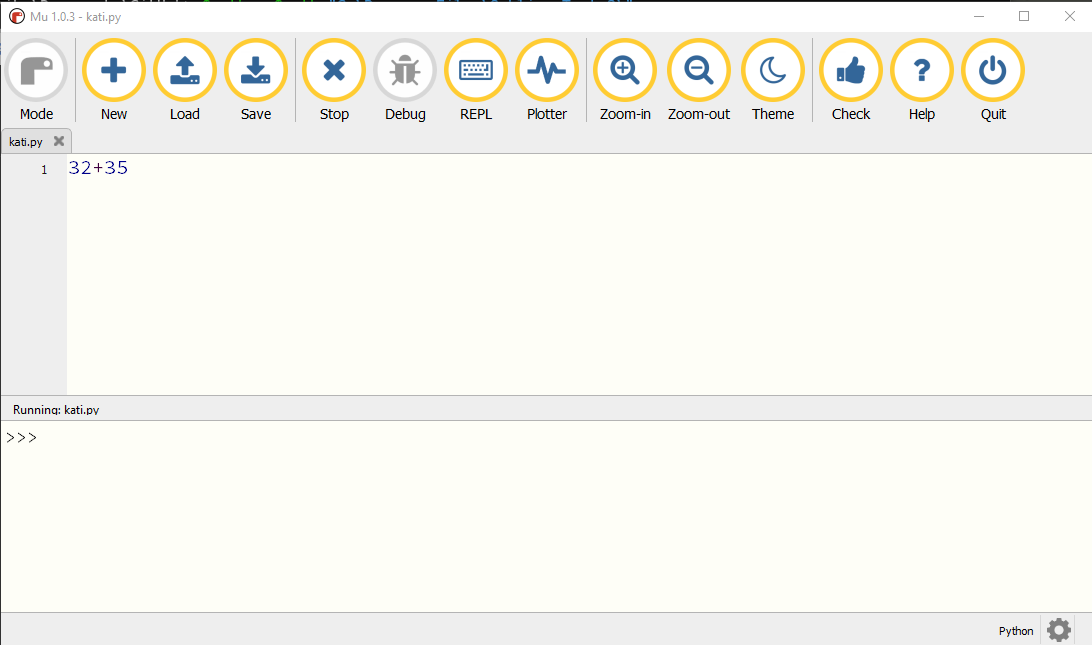
\includegraphics[width=\textwidth]{noprint.png}
\caption{Η εκτέλεση δεν δίνει κάποιο αποτέλεσμα}
\label{noprint}
\end{figure}

Η Python εκτελεί την πράξη $32+35$, και υπολογίζει το αποτέλεσμα. Αν δεν το έκανε και υπήρχε κάποιο πρόβλημα θα εμφάνιζε κάποιο μήνυμα λάθους στο REPL. Το υπολογισμένο αποτέλεσμα δεν εμφανίζεται. Για να εμφανιστεί το αποτέλεσμα πρέπει να χρησιμοποιήσεις την εντολή print (εκτύπωσε). Η εντολή print εκτελείται ως εξής:
\begin{lstlisting}
print(32+35)
\end{lstlisting}
Γράφουμε δηλαδή, print ανοίγουμε παρένθεση, γράφουμε αυτό που θέλουμε να εκτυπωθεί και κλείνουμε την παρένθεση. Όταν εκτελέσουμε το πρόγραμμα με την print τότε εμφανίζεται το αποτέλεσμα στο REPL (εικόνα \ref{withprint}).
\begin{figure}
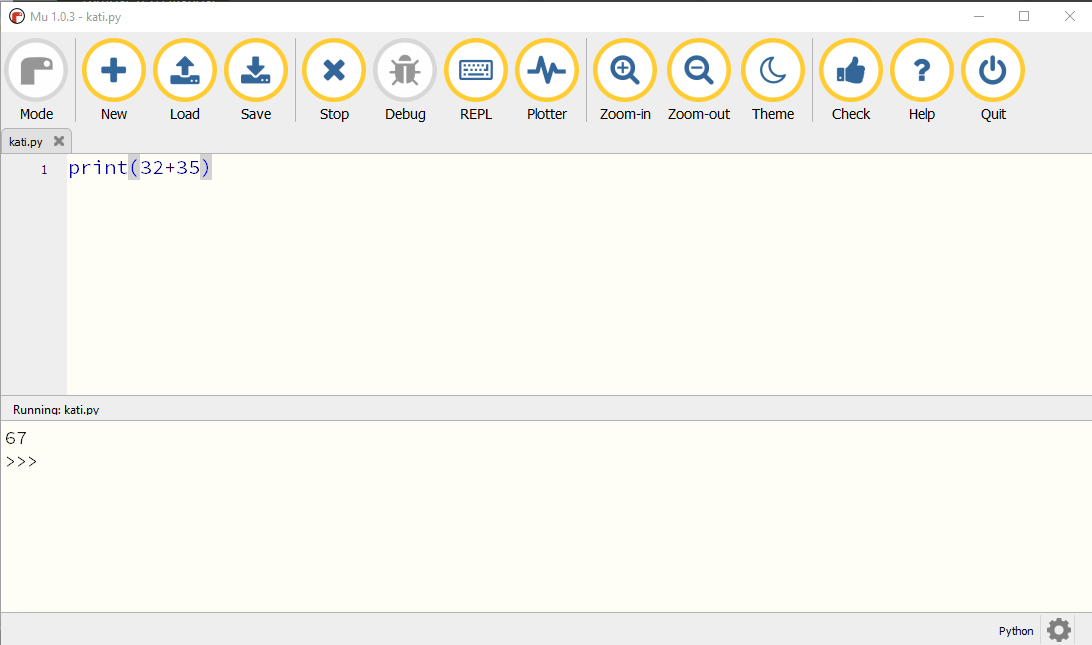
\includegraphics[width=\textwidth]{withprint.png}
\caption{Η εκτέλεση δίνει το αποτέλεσμα της πράξης}
\label{withprint}
\end{figure}
Μόλις έγραψες το πρώτο σου πρόγραμμα στην Python. Μάλιστα το πρόγραμμά σου κάνει κάτι. Υπολογίζει το αποτέλεσμα της πράξης $32+35$.
Μπορείς να αποθηκεύσεις το πρόγραμμά σου στον υπολογιστή σου κάνοντας κλικ στο εικονίδιο Save του Mu (εικόνα \ref{savewithmu}).
\begin{figure}
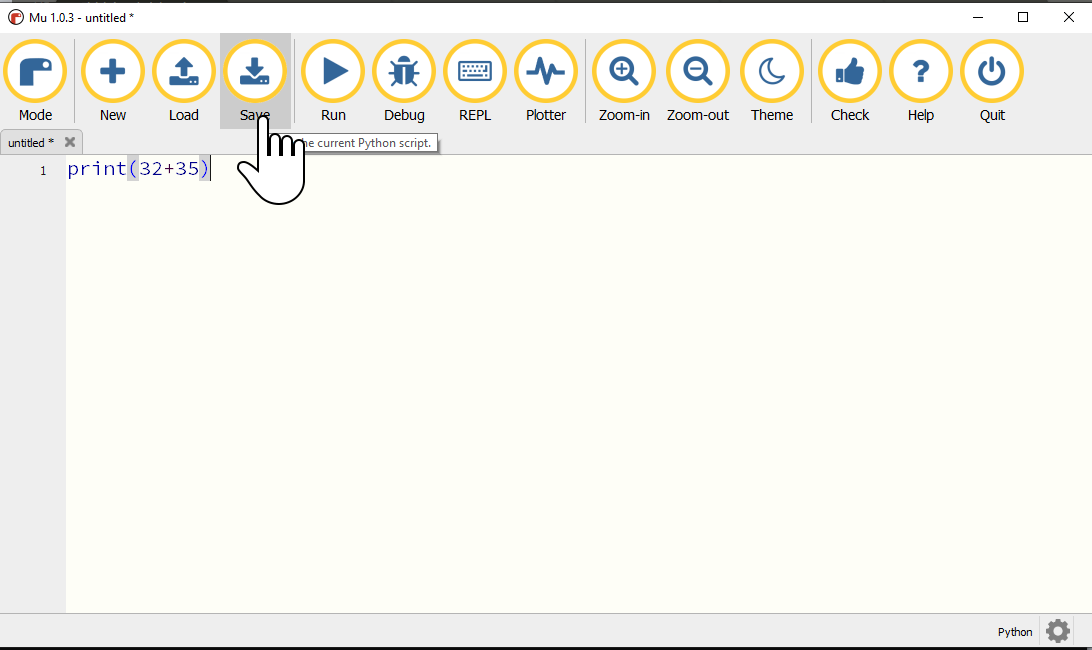
\includegraphics[width=\textwidth]{save.png}
\caption{Αποθήκευση με το Mu}
\label{savewithmu}
\end{figure}

\section{Απαρίθμηση}
Είδαμε ότι η Python μπορεί να κάνει πολύ γρήγορα, πολύπλοκες πράξεις ακόμη και με δυνάμεις, αλλά δεν είδαμε ακόμη τις απλές ασκήσεις που υπάρχουν στις πρώτες σελίδες του βιβλίου. Όπως για παράδειγμα ποιοι είναι οι τρεις προηγούμενοι αριθμοί του 289 και ποιο οι δύο επόμενοι \sel{13}.

Τώρα που μάθαμε να γράφουμε προγράμματα σε Python μπορούμε να αντιμετωπίσουμε αυτό το πρόβλημα με το παρακάτω πρόγραμμα:
\begin{lstlisting}
print(289-3)
print(289-2)
print(289-1)
print(289+1)
print(289+2)
\end{lstlisting}
που δίνει το αποτέλεσμα
\begin{lstlisting}
286
287
288
290
291
\end{lstlisting}

Πιο σωστό θα ήταν να γράψουμε ποιοι αριθμοί είναι οι προηγούμενοι και ποιοι οι επόμενοι. Σε αυτή την περίπτωση θα γράψουμε τις παρακάτω εντολές.
\begin{lstlisting}
print("Οι  προηγούμενοι αριθμοί είναι:")
print(289-3)
print(289-2)
print(289-1)
print("Οι επόμενοι αριθμοί είναι:")
print(289+1)
print(289+2)
\end{lstlisting}

Για να εμφανίσει η print τις λέξεις που θέλουμε πρέπει να τις βάλουμε μέσα σε εισαγωγικά. Η Python υποστηρίζει είτε μονά εισαγωγικά, είτε διπλά. Αυτά εισάγονται συνήθως με το ίδιο κουμπί του πληκτρολογίου (κοντά στο ENTER), είτε με SHIFT ή χωρίς. Θυμήσου να κλείνεις τα εισαγωγικά με τον ίδιο τρόπο που τα άνοιξες. Στο πρόγραμμα Mu τα εισαγωγικά αυτά δεν φαίνονται όπως σε άλλα πρόγραμματα σαν `Εισαγωγικά' ή ``Εισαγωγικά " ή <<Εισαγωγικά>>, αλλά φαίνονται κάπως πιο απλά και ίδια στο άνοιγμα και το κλείσιμο \lstinline{'Εισαγωγικά'} ή  \lstinline{"Εισαγωγικά"}. 

Αν θέλουμε να αλλάξουμε το 289 και να βάλουμε έναν άλλο αριθμό,π.χ. το 132 θα πρέπει να αντικαταστήσουμε το 289 μέσα σε όλες τις εντολές print με το 132.
\begin{lstlisting}
print("Οι προηγούμενοι αριθμοί είναι:")
print(132-3)
print(132-2)
print(132-1)
print("Οι επόμενοι αριθμοί είναι:")
print(132+1)
print(132+2)
\end{lstlisting}

Υπάρχει όμως ένας καλύτερος τρόπος, ο τρόπος αυτός είναι να δώσουμε ένα όνομα στον αριθμό μας. Μπορούμε να πούμε ότι το n είναι το όνομα του αριθμού. Αυτό γίνεται με την εντολή \lstinline{n=132}. Τότε το πρόγραμμά μας γίνεται:
\begin{lstlisting}
n = 132
print("Οι προηγούμενοι αριθμοί είναι:")
print(n-3)
print(n-2)
print(n-1)
print("Οι επόμενοι αριθμοί είναι:")
print(n+1)
print(n+2)
\end{lstlisting}

Μετά την εντολή \lstinline{n=132} η Python ξέρει ότι το n είναι ένα όνομα για το 132 και μπορεί να κάνει πράξεις με αυτό. Για παράδειγμα n+1 κάνει τώρα 133.

Αν θέλουμε να κάνουμε τώρα το ίδιο πρόγραμμα αλλά όχι για το 132 αλλά για το 210, χρειάζεται να αλλάξουμε μόνο μία γραμμή και το πρόγραμμά μας να γίνει ως εξής:
\begin{lstlisting}
n = 210
print("Οι προηγούμενοι αριθμοί είναι:")
print(n-3)
print(n-2)
print(n-1)
print("Οι επόμενοι αριθμοί είναι:")
print(n+1)
print(n+2)
\end{lstlisting}

Στην Python, όταν δίνουμε ένα όνομα σε έναν αριθμό (με τον τελεστή =) τότε δημιουργούμε μια μεταβλητή. Η μεταβλητή έχει ένα όνομα, στην περίπτωσή μας το n, και μια τιμή, στην περίπτωσή μας το 210.

Αν αντί για τους επόμενους δύο αριθμούς θέλαμε τους επόμενους \textbf{δέκα} θα γράφαμε ένα πρόγραμμα όπως το παρακάτω:
\begin{lstlisting}
n = 210
print(n)
print(n+1)
print(n+2)
print(n+3)
print(n+4)
print(n+5)
print(n+6)
print(n+7)
print(n+8)
print(n+9)
print(n+10)
\end{lstlisting}
Το παραπάνω πρόγραμμα εμφανίζει και τον αριθμό μας n, δηλαδή το 210.

Για να μην γράφουμε πολλές εντολές όταν κάνουμε το ίδιο πράγμα χρησιμοποιούμε την εντολή for.
Το πρόγραμμά μας με την for μπορεί να γίνει:
\begin{lstlisting}
n = 210
for i in 0,1,2,3,4,5,6,7,8,9,10:
    print(n+i)
\end{lstlisting}
Όταν γράψεις την for στην Python θα πρέπει να δηλώσεις ποιες εντολές θα εκτελεστούν πολλές φορές. Αυτή η δήλωση γίνεται βάζοντας αυτές τις εντολές λίγο πιο μέσα χρησιμοποιώντας το πλήκτρο κενό ή το πλήκτρο tab. Μια καλή πρακτική είναι να βάζεις τέσσερα κενά. Έτσι, πριν την εντολή \lstinline{print(n+i)} βάζεις τέσσερα κενά δηλαδή \lstinline[showspaces=true]{    print(n+i)}.
Το πρόγραμμα αυτό σημαίνει πως για το i μέσα στο σύνολο 0, 1, 2, 3, \ldots 10 και με αυτή τη σειρά εμφάνισε το n+i. Έτσι το αποτέλεσμα είναι το αναμενόμενο
\begin{lstlisting}
210
211
212
213
214
215
216
217
218
219
220
\end{lstlisting}

Στην Python υπάρχει ένας πιο εύκολος τρόπος να γράψουμε τους αριθμούς από το 0 έως το 10. Αυτός ο τρόπος είναι η εντολή range και συγκεκριμένα η range(11). Η range(11) φτιάχνει τους αριθμούς από το 0 μέχρι το 10 οι οποίοι είναι σε πλήθος 11. 
Έτσι το πρόγραμμά μας γίνεται:
\begin{lstlisting}
n = 210
for i in range(11):
    print(n+i)
\end{lstlisting}

Mπορούμε και να μετρήσουμε τους πρώτους 100 αριθμούς ως εξής:
\begin{lstlisting}
for i in range(100):
    print(i)
\end{lstlisting}

Σκέψου αν θα δεις τον αριθμό 100 στο αποτέλεσμα του παραπάνω προγράμματος.

Μπορούμε να δούμε αριθμούς εύκολα με την Python αλλά θα χρειαστεί ξεχωριστό πρόγραμμα αν θέλουμε να εμφανίζεται το λεκτικό  για κάθε αριθμό.

Ένα τέτοιο πρόγραμμα είναι το παρακάτω:
\begin{lstlisting}
print('μηδέν')
print('ένα')
print('δύο')
print('τρία')
print('τέσσερα')
print('πέντε')
print('έξι')
print('εφτά')
print('οχτώ')
print('εννιά')
print('δέκα')
print('έντεκα')
print('δώδεκα')
print('δεκατρία')
print('δεκατέσσερα')
print('δεκαπέντε')
print('δεκαέξι')
print('δεκαεφτά')
print('δεκαοχτώ')
print('δεκαεννιά')
\end{lstlisting}

Το παραπάνω πρόγραμμα μπορεί να γίνει πιο μαζεμένο με τη χρήση λίστας. Μια λίστα μπορεί να περιέχει τα λεκτικά για κάθε αριθμό. Η λίστα στην Python σημειώνεται με τις τετράγωνες αγκύλες \[ και \]. Τα στοιχεία της χωρίζονται με κόμμα. Έτσι η λίστα που θέλουμε τώρα είναι η εξής:
\begin{lstlisting}
lektika = ['μηδέν','ένα','δύο','τρία','τέσσερα','πέντε','έξι','εφτά','οχτώ','εννιά','δέκα','έντεκα','δώδεκα','δεκατρία','δεκατέσσερα','δεκαπέντε','δεκαέξι','δεκαεφτά','δεκαοχτώ','δεκαεννιά']
\end{lstlisting}
Χρησιμοποιούμε τις τετράγωνες αγκύλες και τον αριθμό του στοιχείου που θέλουμε να προσπελάσουμε σε μια λίστα. Η αρίθμηση της λίστας ξεκινάει από το 0. Έτσι, στη λίστα που βλέπουμε παραπάνω το lektika[0] θα είναι η λέξη 'μηδέν' (θυμηθείτε τα εισαγωγικά), το lektika[1] θα είναι η λέξη 'ένα' κ.ο.κ.

Αν θέλετε μπορείτε να κάνετε μια μικρή δοκιμή στο REPL.
\begin{lstlisting}
>>>lektika = ['μηδέν','ένα','δύο']
>>>lektika[0]
μηδέν
>>>lektika[1]
ένα
>>>lektika[2]
δύο
\end{lstlisting}
Με τη χρήση της λίστας μπορούμε να εμφανίσουμε τους αριθμούς με τη σειρά χρησιμοποιώντας την εντολή for.
\begin{lstlisting}
lektika = ['μηδέν','ένα','δύο','τρία','τέσσερα','πέντε','έξι','εφτά',
'οχτώ','εννιά','δέκα','έντεκα','δώδεκα','δεκατρία',
'δεκατέσσερα','δεκαπέντε','δεκαέξι','δεκαεφτά','δεκαοχτώ',
'δεκαεννιά']
for i in range(20):
    print(lektika[i])
\end{lstlisting}

Όμως παρότι δεν γράφουμε είκοσι φορές την εντολή print πάλι δίνουμε όλα τα ονόματα στο πρόγραμμά μας βάζοντάς τα σε μια λίστα. Μπορούμε να το αποφύγουμε υπολογίζοντας το λεκτικό. Από το δώδεκα και μέτα το λεκτικό ενός αριθμού i είναι το 'δέκα' και μετά το λεκτικό του αριθμού i-10. Για παράδειγμα, το δεκαοχτώ είναι το 'δέκα' ακολουθούμενο από το λεκτικό του αριθμού που προκ΄κυπτει αν αφαιρέσουμε 10 από το 18.
Το πρόγραμμά μας γίνεται:
\begin{lstlisting}
lektika = ['μηδέν','ένα','δύο','τρία','τέσσερα','πέντε','έξι','εφτά',
'οχτώ','εννιά','δέκα','έντεκα','δώδεκα','δεκατρία',
'δεκατέσσερα','δεκαπέντε','δεκαέξι','δεκαεφτά','δεκαοχτώ',
'δεκαεννιά']
for i in range(20):
    if i<=12:
        print(lektika[i])
    else:
        print('δέκα'+lektika[i-10])
\end{lstlisting}

Μάλιστα, το πρόγραμμα υπολογίζει τα λεκτικά από το 13 και μετά και δεν χρειάζεται να τα θυμάται. Μπορούμε να τα διαγράψουμε από τη λίστα.
\begin{lstlisting}
lektika = ['μηδέν','ένα','δύο','τρία','τέσσερα','πέντε','έξι','εφτά',
'οχτώ','εννιά','δέκα','έντεκα','δώδεκα']
for i in range(20):
    if i > 12:
        print('δέκα'+lektika[i-10])
    else:
        print(lektika[i])
\end{lstlisting}

Τώρα μπορούμε να πάμε μέχρι το 29.
\begin{lstlisting}
lektika = ['μηδέν','ένα','δύο','τρία','τέσσερα','πέντε','έξι','εφτά',
'οχτώ','εννιά','δέκα','έντεκα','δώδεκα']
for i in range(30):
    if i>20:
        print('είκοσι' + lektika[i-20])
    elif i > 12:
        print('δέκα'+lektika[i-10])
    else:
        print(lektika[i])
\end{lstlisting}
Το elif είναι συντομογραφία για το else if. Στο σημείο που το έβαλες τώρα σημαίνει αν το i δεν είναι μεγαλύτερο του 20 (else) και είναι μεγαλύτερο από το 12 (if). Άρα το \lstinline{print('δέκα'+lektika[i-10])} γίνεται μόνο αν το i είναι μικρότερο ή ίσο του 20 και μεγαλύτερο από 12.
Το αποτέλεσμα φαίνεται παρακάτω:
\begin{lstlisting}
 ένα  
 δύο 
 τρία 
 τέσσερα 
 πέντε 
 έξι 
 εφτά 
 οχτώ 
 εννιά 
 δέκα 
 έντεκα 
 δώδεκα 
 δέκατρία 
 δέκατέσσερα 
 δέκαπέντε 
 δέκαέξι 
 δέκαεφτά 
 δέκαοχτώ 
 δέκαεννιά 
  (*@\textcolor{blue}{δέκαδέκα}@*) 
 είκοσιένα 
 είκοσιδύο 
 είκοσιτρία 
 είκοσιτέσσερα 
 είκοσιπέντε 
 είκοσιέξι 
 είκοσιεφτά 
 είκοσιοχτώ 
 είκοσιεννιά 
\end{lstlisting}
Οπότε καταλαβαίνουμε ότι το είκοσι χρειάζεται ειδικό χειρισμό. Με τη χρήση της elif μπορούμε να βάλουμε και ειδικό χειρισμό για το 20.
\begin{lstlisting}
lektika = ['μηδέν','ένα','δύο','τρία','τέσσερα','πέντε','έξι','εφτά',
'οχτώ','εννιά','δέκα','έντεκα','δώδεκα']
for i in range(30):
    if i>20:
        print('είκοσι' + lektika[i-20])
    elif i==20:
        print('είκοσι')
    elif i > 12:
        print('δέκα'+lektika[i-10])
    else:
        print(lektika[i])
\end{lstlisting}



\section{Στρογγυλοποίηση}
Το βιβλίο των Μαθηματικών της Α' Γυμνασίου αναφέρει πως
Για να στρογγυλοποιήσουμε έναν φυσικό αριθμό \sel{12}:
\begin{enumerate}
	\item Προσδιορίζουμε την τάξη στην οποία θα γίνει η στρογγυλοποίηση
	\item Εξετάζουμε το ψηφίο της αμέσως μικρότερης τάξης
	\item Αν αυτό το ψηφίο είναι μικρότερο του 5 (δηλαδή 0, 1, 2, 3 ή 4) το ψηφίο αυτό και όλα τα ψηφία των υπόλοιπων τάξεων μηδενίζονται.
	\item Αν είναι μεγαλύτερο ή ίσο του 5 (δηλαδή 5, 6, 7, 8 ή 9) το ψηφίο αυτό και όλα τα ψηφία των υπόλοιπων τάξεων αντικαθίστανται από το 0 και το ψηφίο της τάξης στρογγυλοποίησης αυξάνεται κατά 1.
\end{enumerate}

Ας πούμε ότι θέλουμε να στρογγυλοποιήσουμε τον αριθμό 454.018.512 στα εκατομμύρια. Η απάντηση που περιμένουμε είναι 454 εκατομμύρια.
Για να τα καταφέρουμε θα χρησιμοποιήσουμε την διαίρεση. Όμως στην Python υπάρχουν \emph{δύο} διαιρέσεις μία με το σύμβολο / και μία με το σύμβολο //. Ας δούμε τις διαφορές τους στο REPL.
\begin{lstlisting}
>>> x = 454018512
>>> print(x/1000000)
454.018512
>>> print(x//1000000)
454
\end{lstlisting}
Η <<κανονική>> διαίρεση, με τη μία κάθετο /, δίνει το αποτέλεσμα της διαίρεσης με τα δεκαδικά ψηφία. Η <<ακέραια>> διαίρεση δίνει μόνο τον ακέραιο αριθμό. Δεν μπορούμε να πούμε ότι η ακέραια διαίρεση θα μας δώσει την στρογγυλοποίηση γιατί η ακέραια διαίρεση δεν στρογγυλοποιεί τα δεκαδικά ψηφία αλλά τα απορρίπτει εντελώς. Έτσι, ακόμη και αν είχαμε 454918512 κατοίκους η ακέραια διαίρεση θα δώσει 454 αντί για το στρογγυλοποιημένο που είναι 455.
\begin{lstlisting}
>>> x = 454918512
>>> print(x/1000000)
454.918512
>>> print(x//1000000)
454
\end{lstlisting}

Χρειάζεται επομένως να δούμε το ψηφίο της αμέσως χαμηλότερης τάξης το οποίο είναι το πρώτο δεκαδικό της κανονικής διαίρεσης. Για να το απομονώσουμε αφαιρούμε από το αποτέλεσμα της κανονικής διαίρεσης το ακέραιο μέρος.
\begin{lstlisting}
>>> x = 454018512
>>> x / 1000000 - x // 1000000
0.018511999999986983
\end{lstlisting}
Οπότε τώρα έχουμε δύο ενδεχόμενα αν το αποτέλεσμα αυτής της πράξης είναι μικρότερο από 0.5 όπως παραπάνω τότε το αποτέλεσμα που ψάχνουμε είναι το αποτέλεσμα της ακέραιας διαίρεσης. Αλλιώς πρέπει να προσθέσουμε ένα στο αποτέλεσμα της ακέραιας διαίρεσης.
Αυτό γίνεται με την εντολή if, που σημαίνει στα αγγλικά αν. Για ευκολία μπορούμε να ονομάσουμε d την διαφορά των δύο διαιρέσεων με την εντολή:
\begin{lstlisting}
d = x / 1000000 - x // 1000000
\end{lstlisting}
Επειδή το πρόγραμμα γίνεται μεγαλύτερο τώρα θα το γράψουμε στο πάνω παράθυρο του Mu.
\begin{lstlisting}
x = 454018512
d = x / 1000000 - x // 1000000
if d < 0.5:
    print(x // 1000000)
else:
    print(x // 1000000 + 1)
\end{lstlisting}
Την \lstinline{if} την γράφουμε ως εξής:
\begin{lstlisting}
if συνθήκη:
    εντολές που εκτελούνται
    αν ισχύει η συνθήκη
else:
    εντολές που εκτελούνται
    αν δεν ισχύει η συνθήκη
\end{lstlisting}
Θυμήσου να βάζεις την άνω κάτω τελεία μετά τη συνθήκη και μετά τη λέξη else που σημαίνει αλλιώς.

Αν στο ίδιο πρόγραμμα και βάλεις αντί για 454.018.512 τον αριθμό 454.918.512 θα δεις ότι θα εμφανιστεί το σωστό αποτέλεσμα (455).

Αν θέλεις στρογγυλοποίηση στις χιλιάδες τότε το πρόγραμμά σου γίνεται:
\begin{lstlisting}
x = 454018512
d = x / 1000 - x // 1000
if d < 0.5:
    print(x // 1000)
else:
    print(x // 1000 + 1)
\end{lstlisting}
και το αποτέλεσμα είναι 454019.

\begin{exercise}
Για να γίνει το 454.018.512, 450 εκατομμύρια \sel{12} η στρογγυλοποίηση γίνεται στις δεκάδες των εκατομμυρίων. Μπορείς να γράψεις ένα πρόγραμμα που να στρογγυλοποιεί αριθμούς στις δεκάδες των εκατομμυρίων;
\end{exercise}

\section{Επανάληψη στις πράξεις}
\begin{exercise}
Συμπλήρωσε τον πίνακα τα τετράγωνα και τους κύβους των αριθμών από το 8 μέχρι το 25 \sel{22}.
\end{exercise}
\begin{lstlisting}
for a in range(8,26):
    print(a**2,end =" ")
print()
print()
for a in range(8,26):
    print(a**3,end=" ")
\end{lstlisting}
Το αποτέλεσμα αυτού του προγράμματος είναι:

\begin{lstlisting}
64 81 100 121 144 169 196 225 256 289 324 361 400 441 484 529 576 625 

512 729 1000 1331 1728 2197 2744 3375 4096 4913 5832 6859 8000 9261 
10648 12167 13824 15625
\end{lstlisting}

Η εντολή print μπορεί να πάρει περισσότερα από ένα ορίσματα, το πρώτο όρισμα είναι αυτό που θα εμφανίσει. Το δεύτερο όρισμα που δώσαμε είναι το end και το ορίσαμε ίσο με το κενό (\lstinline{end=" "}) που σημαίνει ότι η print όταν εμφανίσει το πρώτο όρισμα δεν θα αλλάξει γραμμή αλλά θα αφήσει ένα κενό. Η εντολή print() αλλάζει απλά γραμμή.
\begin{exercise}
Βρες τα τετράγωνα των αριθμών 10,20,30,40,50,60,70,80 και 90 \sel{22}.
\end{exercise}
Το πρόγραμμα είναι το εξής:
\begin{lstlisting}
for i in range(10,100,10):
    print(i**2,end=',')
\end{lstlisting}
και το αποτέλεσμα της εκτέλεσης του προγράμματος είναι
\begin{lstlisting}
100,400,900,1600,2500,3600,4900,6400,8100,
\end{lstlisting}

\begin{exercise}
Βρες τους κύβους των αριθμών 10,20,30,40,50
\end{exercise}

\begin{lstlisting}
for i in range(10,60,10):
    print(i**3,end=', ')  
\end{lstlisting}
Το αποτέλεσμα της εκτέλεσης είναι:
\begin{lstlisting}
1000, 8000, 27000, 64000, 125000, 
\end{lstlisting}

\section{Ανάπτυγμα}
\begin{exercise}\sel{21}Να γραφεί το ανάπτυγμα του αριθμόύ 7.604 με χρήση των δυνάμεων του 10.
\end{exercise}
Η απάντηση είναι $7\cdot 10^3 + 6\cdot 10^2 + 0\cdot 10^1 + 4$. 
%\chapter{Η έννοια του κλάσματος}
\section{Εισαγωγή}
\begin{exercise}
Ένα βράδυ τρεις φίλοι αγοράζουν μια πίτσα και την χωρίζουν σε οκτώ κομμάτια. Ο ένας έφαγε το ένα, ο δεύτερος τα τρία και ο τρίτος δύο κομμάτια από αυτά που περίσσεψαν.

1. Μπορείς να βρεις το μέρος της πίτσας που έφαγε ο καθένας;

 2. Τι μέρος της πίτσας περίσσεψε;
 \end{exercise}

Ο πρώτος έφαγε το $\frac{1}{8}$ ο δεύτερος τα $\frac{3}{8}$ και ο τρίτος τα $\frac{2}{8}$.
Επομένως και οι τρεις μαζί έφαγαν $1+3+2=6$ κομμάτια, δηλαδή τα $\frac{6}{8}$ της πίτσας. Άρα περίσσεψαν τα υπόλοιπα δύο κομμάτια από τα οκτώ, δηλαδή τα $\frac{2}{8}$ της πίτσας.

Πώς μπορούν να γίνουν πράξεις με κλάσματα στην python; Με τις γνώσεις που ήδη έχουμε εκτελούμε τις παρακάτω εντολές:
\begin{lstlisting}
>>> 1/8
0.125
>>> 3/8
0.375
>>> 2/8
0.25
\end{lstlisting}
Θυμηθείτε ότι η python χρησιμοποιεί την τελεία για τους δεκαδικούς!
Τι μέρος της πίτσας περίσσεψε;
\begin{lstlisting}
>>> 1 - 1/8 - 3/8 - 2/8
0.25
\end{lstlisting}

Όμως, υπάρχει τρόπος η python να υπολογίζει κλάσματα. Απλά θα πρέπει να εισαχθεί το κατάλληλο module. Στην python υπάρχει διαθέσιμο τέτοιο module και ονομάζεται fractions. Για το δεύτερο ερώτημα λοιπόν μπορούμε να κάνουμε το εξής:
\begin{lstlisting}
>>> import fractions
>>> prwtos = fractions.Fraction(1,8)
>>> deuteros = fractions.Fraction(3,8)
>>> tritos = fractions.Fraction(2,8)
>>> 1 - prwtos - deuteros - tritos
Fraction(1, 4)
\end{lstlisting}
Έτσι η python υπολογίζει το αποτέλεσμα με τη μορφή κλάσματος και Fraction(1,4) σημαίνει $\frac{1}{4}$.

Παρατηρείτε ότι γράφουμε το όνομα του module στη συνέχεια την τελεία ``.'' και τέλος το Fraction. Με αυτόν τον τρόπο καλούμε κάτι που υπάρχει μέσα στο module. Υπάρχει όμως και ένας πιο εύκολος τρόπος για να εισάγουμε μόνο τις λειτουργίες που θέλουμε από ένα module και να τις καλούμε.
\begin{lstlisting}
>>> from fractions import Fraction
>>> prwtos = Fraction(1,8)
>>> deuteros = Fraction(3,8)
>>> tritos = Fraction(2,8)
>>> 1 - prwtos - deuteros - tritos
Fraction(1, 4)
\end{lstlisting}
Χρειάζεται προσοχή μόνο αν υπάρχουν περισσότερα από ένα module που πιθανόν να έχουν την ίδια λειτουργία κάτι που δεν ισχύει σε αυτήν την περίπτωση. 

\begin{exercise}
Μια σοκολάτα ζυγίζει 120 gr και έχει 6 ίσα κομμάτια.
(α)   Ποιο μέρος της σοκολάτας είναι το κάθε κομμάτι;
(β)   Πόσα κομμάτια πρέπει να κόψουμε για να πάρουμε 40 gr;
\end{exercise}

Το μέρος της σοκολάτας είναι $\frac{1}{6}$ για να βρούμε πόσα κομμάτια χρειαζόμαστε για 40gr θα πρέπει να βρούμε το βάρος του κομματιού που είναι $\frac{1}{6}\cdot 120$. Τέλος, τα κομμάτια που πρέπει να κόψουμε προκύπτουν από τη διαίρεση των 40 γραμμαρίων με το βάρος του κάθε κομματιού.

\begin{lstlisting}
from fractions import Fraction

sok = Fraction(1,6)
print(sok)
baroskommatiou = sok * 120
kommatia = 40 / baroskommatiou
print('Θα κόψω ' + str(kommatia) + ' κομμάτια!')
\end{lstlisting}
το αποτέλεσμα θα είναι το εξής:
\begin{lstlisting}
1/6
Θα κόψω 2 κομμάτια!
\end{lstlisting}

\begin{exercise}Το καμπαναριό μιας εκκλησίας έχει ύψος 20 m, ενώ η εκκλησία έχει ύψος τα Εικόνα του ύψους του καμπαναριού. Ποιο είναι το ύψος της εκκλησίας;\end{exercise}

\begin{lstlisting}
from fractions import Fraction

>>> kampanario = Fraction(3,5)*20
>>> print(kampanario)
12
\end{lstlisting}
Άρα το ύψος της εκκλησίας είναι 12m.

Στη συνέχεια η εντολή from fractions import Fraction θα υποννοείται ώστε να μην επαναλαμβάνεται συνεχώς. Αν τυχόν την ξεχάσετε το αποτέλεσμα θα έχει το εξής σφάλμα:
\begin{lstlisting}
NameError: name 'Fraction' is not defined
\end{lstlisting}
\begin{exercise} Μια δεξαμενή πετρελαίου σε μια πολυκατοικία, χωράει 2000 lt. Ο διαχειριστής σε μια μέτρηση βρήκε ότι ήταν γεμάτη κατά τα $\frac{3}{4}$. Πόσα λίτρα πετρέλαιο είχε η δεξαμενή;
\end{exercise}
\begin{lstlisting}
>>> dexameni = Fraction(3,4)*2000
>>> print(dexameni)
1500
\end{lstlisting}

Η δεξαμενή έχει 1500 lt.

\begin{exercise}
Tα $\frac{3}{5}$ του κιλού τυρί κοστίζουν 27 €. 

Πόσο κοστίζουν τα $\frac{8}{9}$ του κιλού;
\end{exercise}

\begin{lstlisting}
>>> enaPempto = Fraction(27,3)
>>> tyri = 5*enaPempto
>>> oktwEnata = Fraction(8,9)*tyri
>>> print(oktwEnata)
40
\end{lstlisting}
Τα $\frac{8}{9}$ του τυριού κοστίζουν 40 ευρώ.
\section{Άσκήσεις}
\begin{exercise}
Είναι τα κλάσματα $\frac{3}{4}$, $\frac{2}{3}$, $\frac{7}{9}$, $\frac{10}{9}$, $\frac{18}{20}$ όλα μικρότερα της μονάδας:
\end{exercise}
\begin{lstlisting}
>>> print(Fraction(3,4)<1)
True
>>> print(Fraction(2,3)<1)
True
>>> print(Fraction(7,9)<1)
True
>>> print(Fraction(10,9)<1)
False
>>> print(Fraction(18,20)<1)
True
\end{lstlisting}

\begin{exercise}Τι κλάσμα των μαθητών της τάξης 28 μαθητών είναι οι 4 απόντες;\end{exercise}

\begin{lstlisting}
>>> print(Fraction(4,28))
1/7
\end{lstlisting}

Παρατηρούμε ότι η εντολή Fraction(4,28) κάνει απλοποίηση κλάσματος.

> Αν το $\frac{1}{5}$ ενός κιλού καρύδια είναι 14 καρύδια, το κιλό περιέχει 70 καρύδια;
\begin{lstlisting}
>>> print(14*5 == 70)
\end{lstlisting}
Ναι.

\begin{exercise}
Βρες ποιο μέρος του κιλού είναι τα: (α) 100, (β) 250, (γ) 500, (δ) 600 γραμμάρια.

\end{exercise}

\begin{lstlisting}
>>> print(Fraction(100,1000))
1/10
>>> print(Fraction(250,1000))
1/4
>>> print(Fraction(500,1000))
1/2
>>> print(Fraction(600,1000)).
3/5
\end{lstlisting}

\begin{exercise}
Ποιο μέρος: (α) του μήνα, (β) του εξαμήνου, (γ) του έτους είναι οι 15 ημέρες;
\end{exercise}

\begin{lstlisting}
>>> print(Fraction(15,30))
1/2
>>> print(Fraction(15,180))
1/12
>>> print(Fraction(15,365))
3/73
\end{lstlisting}

\begin{exercise}
Ένα κατάστημα κάνει έκπτωση στα είδη του ίση με τα $\frac{2}{5}$ της αρχικής τιμής τους. Ένα φόρεμα κόστιζε 90 € πριν την έκπτωση. Υπολόγισε πόσα ευρώ έκπτωση έγινε στο φόρεμα και πόσο θα πληρώσουμε για να το αγοράσουμε.
\end{exercise}
\begin{lstlisting}
>>> ekpt = Fraction(2,5)*90
>>> print("Η έκπτωση είναι: " + str(ekpt) + " ευρώ!")
Η έκπτωση είναι: 36 ευρώ!
>>> plir = 90 - ekpt
>>> print("Θα πληρώσουμε: " + str(plir) + " ευρώ!")
Θα πληρώσουμε: 54 ευρώ!
\end{lstlisting}

\begin{exercise}
Σε μία τάξη τα $\frac{3}{8}$ των μαθητών μαθαίνουν αγγλικά. Να βρεις πόσους μαθητές έχει η τάξη, αν γνωρίζεις ότι αυτοί που μαθαίνουν αγγλικά είναι 12 μαθητές.
\end{exercise}

\begin{lstlisting}
>>> print(Fraction(8,3)*12)
32
\end{lstlisting}

\begin{exercise}
Σε ένα ορθογώνιο παραλληλόγραμμο η μια πλευρά του είναι 33 εκατοστά και η άλλη τα $\frac{3}{11}$ της πρώτης. Να βρεις την περίμετρο του ορθογωνίου.
\end{exercise}

\begin{lstlisting}
>>> plevra1 = 33
>>> plevra2 = Fraction(3,11)*plevra1
>>> perimetros = 2*(plevra1 + plevra2)
>>> print(perimetros)
84
\end{lstlisting}

\section{Ισοδύναμα κλάσματα}

\begin{exercise}
Να εξετάσετε αν τα κλάσματα: α) $\frac{3}{5}$ και $\frac{10}{14}$ β) $\frac{3}{8}$ και $\frac{18}{48}$ είναι ισοδύναμα.
\end{exercise}
\begin{lstlisting}
print(Fraction(3,5) == Fraction(10,14))
False
print(Fraction(3,8) == Fraction(18,48))
True
\end{lstlisting}

Έτσι, τα $\frac{3}{5}$ και $\frac{10}{14}$ δεν είναι ισοδύναμα ενώ τα $\frac{3}{8}$ και $\frac{18}{48}$ είναι.

\begin{exercise}Να απλοποιηθεί το κλάσμα $\frac{30}{66}$
\end{exercise}

\begin{lstlisting}
>>> print(Fraction(30,66))
5/11
\end{lstlisting}

\begin{exercise}Να μετατραπούν σε ομώνυμα τα κλάσματα $\frac{3}{5}$, $\frac{2}{3}$ και $\frac{5}{20}$:
\end{exercise}

Επειδή η Fraction κάνει απλοποίηση σε ανάγωγο κλάσμα δεν μπορούμε να επιλέξουμε παρονομαστή, γι' αυτό θα κατασκευάσετε μια συνάρτηση η οποία θα τυπώνει το κλάσμα επιλέγοντας τον παρονομαστή.

\begin{lstlisting}
def tiposemeparonomasti(k,p):
  """
  tiposemeparonomasti(k,p)
  Τύπωσε το κλάσμα k με παρονομαστή p
  """
  if p % k.denominator == 0:#αν το p είναι πολλαπλάσιο
                            #του τρέχοντος παρονομαστή (denominator)
                            #τότε μπορούμε να πολλαπλασιάσουμε
                            #όλο το κλάσμα με έναν συντελεστή
    synt = int(p // k.denominator)
    print(str(k.numerator * synt) + '/' + str(k.denominator * synt))
  else:#αν το p δεν είναι πολλαπλάσιο του τρέχοντος παρονομαστή
       #τότε τυπώνουμε το κλάσμα ως έχει
    print(k)
\end{lstlisting}

Το k.denominator είναι ο παρονομαστής του κλάσματος k.

Αφού φτιάξετε τη συνάρτηση tiposemeparonomasti δοκιμάστε:
\begin{lstlisting}
>>> tiposemeparonomasti(Fraction(3,4),12)
9/12
>>> tiposemeparonomasti(Fraction(1,2),20)
10/20
\end{lstlisting}

Για να κάνουμε ομώνυμα τα κλάσματα βρίσκουμε το Ελάχιστο Κοινό Πολλαπλάσιο (Ε.Κ.Π.) των παρονομαστών. 
Η συνάρτηση για το Ε.Κ.Π. είναι η παρακάτω, αφού το Ε.Κ.Π. δύο αριθμών προκύπτει από το γινόμενο τους αφού το διαιρέσουμε με τον μέγιστο κοινό διαιρέτη (Μ.Κ.Δ. - G.C.D.). Μάλιστα η βιβλιοθήκη fractions περιέχει τη συνάρτηση gcd που υπολογίζει το Μ.Κ.Δ. οπότε:
\begin{lstlisting}
from fractions import gcd
def ekp(a,b):
  return(a*b/gcd(a,b))
\end{lstlisting}

Τέλος συνδυάζοντας τα προηγούμενα το συνολικό πρόγραμμα για να κάνουμε ομώνυμα τα κλάσματα $\frac{3}{5}$, $\frac{2}{3}$ και $\frac{5}{20}$ είναι:

\begin{lstlisting}
from fractions import Fraction,gcd
def tiposemeparonomasti(k,p):
  """
  tiposemeparonomasti(k,p)
  Τύπωσε το κλάσμα k με παρονομαστή p
  """
  if p % k.denominator == 0:#αν το p είναι πολλαπλάσιο
                            #του τρέχοντος παρονομαστή (denominator)
                            #τότε μπορούμε να πολλαπλασιάσουμε
                            #όλο το κλάσμα με έναν συντελεστή
    synt = int(p // k.denominator)
    print(str(k.numerator * synt) + '/' + str(k.denominator * synt))
  else:#αν το p δεν είναι πολλαπλάσιο του τρέχοντος παρονομαστή
       #τότε τυπώνουμε το κλάσμα ως έχει
    print(k)

def ekp(a,b):
  return(a*b/gcd(a,b))    
  
a = Fraction(3,5)
b = Fraction(2,3)
c = Fraction(5,20)
    
koinos = ekp(a.denominator,ekp(b.denominator,c.denominator))
tiposemeparonomasti(a,koinos)
tiposemeparonomasti(b,koinos)
tiposemeparonomasti(c,koinos)
\end{lstlisting}

Μπορούμε να εισάγουμε δύο λειτουργίες από την ίδια βιβλιοθήκη χωρίζοντάς τες με κόμμα ",".
Θυμηθείτε ότι σε ένα κλάσμα a το a.denominator είναι ο παρονομαστής.

Το αποτέλεσμα του προγράμματος είναι:

\begin{lstlisting}
36/60
40/60
15/60
\end{lstlisting}

\begin{exercise}
Να εξετάσετε ποια από τα παρακάτω κλάσματα είναι ισοδύναμα:

(α)$\frac{2}{3},\frac{18}{27}$, 

(β)$\frac{3}{4}$, $\frac{1}{2}$, 

(γ)$\frac{7}{8}$, $\frac{30}{40}$, 

(δ)$\frac{13}{14}$, $\frac{26}{28}$.
\end{exercise}

\begin{lstlisting}
>>> print(Fraction(2,3)==Fraction(18,27))
True
>>> print(Fraction(3,4)==Fraction(1,2))
False
>>> print(Fraction(7,8)==Fraction(30,40))
False
>>> print(Fraction(13,14)==Fraction(26,28))
True
\end{lstlisting}

\begin{exercise}
Να μετατρέψεις καθένα από τα παρακάτω κλάσματα σε ισοδύναμο κλάσμα με παρονομαστή  τον αριθμό 100: 

(α)$\frac{3}{4}$ 

(β)$\frac{8}{5}$ 

(γ)$\frac{4}{20}$ 

(δ)$\frac{5}{2}$ 

(ε)$\frac{60}{75}$

\end{exercise}

Μπορούμε να χρησιμοποιήσουμε την συνάρτηση tiposemeparonomasti
\begin{lstlisting}
>>> tiposemeparonomasti(Fraction(3,4),100)
75/100
>>> tiposemeparonomasti(Fraction(8,5),100)
160/100
>>> tiposemeparonomasti(Fraction(4,20),100)
20/100
>>> tiposemeparonomasti(Fraction(5,2),100)
250/100
>>> tiposemeparonomasti(Fraction(60,75),100)
80/100
\end{lstlisting}

\begin{exercise}Να μετατρέψεις τα παρακάτω κλάσματα σε ισοδύναμα με παρονομαστή τον αριθμό 3:\end{exercise}

\begin{lstlisting}
>>> tiposemeparonomasti(Fraction(10,6),3)
5/3
>>> tiposemeparonomasti(Fraction(50,30),3)
5/3
>>> tiposemeparonomasti(Fraction(18,27),3)
2/3
\end{lstlisting}

\begin{exercise}
Να μετατρέψεις το κλάσμα $\frac{2}{3}$ σε ισοδύναμο κλάσμα με παρονομαστή:(α) 6, και (β) 15.
\end{exercise}

\begin{lstlisting}
>>> tiposemeparonomasti(Fraction(2,3),6)
4/6
>>> tiposemeparonomasti(Fraction(2,3),15)
10/15
\end{lstlisting}

\begin{exercise}
Να απλοποιήσεις τα κλάσματα: (α)$\frac{25}{30}$ (β) $\frac{12}{9}$ (γ) $\frac{32}{56}$
\end{exercise}

\begin{lstlisting}
>>> print(Fraction(25,30))
5/6
>>> print(Fraction(12,9))
4/3
>>> print(Fraction(32,56))
4/7
\end{lstlisting}

\section{Πρόσθεση και αφαίρεση κλασμάτων}

\begin{exercise} Το συνεργείο του Δήμου φύτεψε σε μια μέρα τα $\frac{4}{12}$ μιας πλατείας με λουλούδια. Την επόμενη ήμερα που ο καιρός δεν ήταν καλός φύτεψε μόνο τα $\frac{3}{12}$ της πλατείας. Ποιο τμήμα της πλατείας είχε φυτέψει, συνολικά, στο τέλος της δεύτερης ημέρας;
\end{exercise}

\begin{lstlisting}
>>> print(Fraction(4,12) + Fraction(3,12)(
7/12
\end{lstlisting}

\begin{exercise}Ένα φορτηγό κάλυψε σε μία ώρα τα 2/5 της διαδρομής Πάτρα - Τρίπολη. Ποιο μέρος της διαδρομής του μένει να καλύψει ακόμη;\end{exercise}

\begin{lstlisting}
>>> print(1-Fraction(2,5))
3/5
\end{lstlisting}

\begin{exercise}Μια βρύση γεμίζει, σε 1 ώρα, τα $\frac{2}{5}$ της δεξαμενής. Μια άλλη βρύση γεμίζει το $\frac{1}{3}$ της ίδιας δεξαμενής, επίσης σε 1 ώρα. Αν και οι δύο βρύσες τρέχουν ταυτόχρονα μέσα στη δεξαμενή, τι μέρος της δεξαμενής θα γεμίσουν σε 1 ώρα;
\end{exercise}

\begin{lstlisting}
>>> print(Fraction(2,5)+Fraction(1,3))
11/15
\end{lstlisting}

\begin{exercise}Να υπολογισθεί το άθροισμα 
$$\frac{1}{4}+\frac{2}{4} + 3$$
\end{exercise}

\begin{lstlisting}
>>> print(Fraction(1,4)+Fraction(2,4) + 3)
15/4
\end{lstlisting}

\begin{exercise}Να υπολογισθεί η διαφορά και το άθροισμα των κλασμάτων
$\frac{3}{12}$ και $\frac{7}{20}$.
\end{exercise}

\begin{lstlisting}
>>> print(Fraction(3,12) + Fraction(7,20))
3/5
>>> print(Fraction(7,20) - Fraction(3,12))
1/10
\end{lstlisting}

Για να τυπώσουμε ένα κλάσμα ως μεικτό θα εφαρμόσουμε τα εξής βήματα:
1. Βρίσκουμε το ακέραιο μέρος της διαίρεσης του αριθμητή με τον παρονομαστή έστω $\mu$.
2. Αν το $\mu$ είναι 0 τυπώνουμε το κλάσμα ως έχει (είναι μικρότερο της μονάδας), αλλιώς τυπώνουμε το $\mu$ και στη συνέχεια το κλάσμα που προκύπτει αν από το αρχικό κλάσμα αφαίρεσουμε το $\mu$.

\begin{lstlisting}
def tiposemikto(k):
  m = k.numerator // k. denominator
  if m == 0:
  	print(k)
  else:
  	print(str(m) + " " + str(k-m))
\end{lstlisting}

Για παράδειγμα
\begin{lstlisting}
>>> tiposemikto(Fraction(15,4))
3 3/4
>>> tiposemikto(Fraction(5,2))
2 1/2
>>> tiposemikto(Fraction(38,12))
\end{lstlisting}

\section{Σύγκριση κλασμάτων}

\begin{exercise}
Η Μαρία είπε πως το ροζ χρώμα καταλαμβάνει τα $\frac{9}{48}$, το γαλάζιο τα $\frac{10}{48}$ και το πράσινο τα $\frac{7}{48}$. Ενώ ο Γιάννης είπε ότι το ροζ είναι τα $\frac{3}{16}$, το γαλάζιο τα $\frac{5}{24}$ και το πράσινο το $\frac{1}{8}$ του τετραγώνου.
Ποιος έχει δίκιο και ποιος όχι;
\end{exercise}

\begin{lstlisting}
>>> roz = Fraction(9,48)
>>> print(roz)
3/16
\end{lstlisting}
Άρα και η Μαρία και ο Γιάννης έχουν δίκο όσον αφορά το ροζ χρώμα.

\begin{lstlisting}
>>> galazio = Fraction(10,48)
>>> print(galazio)
5/24
\end{lstlisting}
Άρα και η Μαρία και ο Γιάννης έχουν δίκο όσον αφορά το γαλάζιο χρώμα.

Τέλος, όσον αφορά το πράσινο προκύπτει ότι:
\begin{lstlisting}
>>> prasino = Fraction(7,48)
>>> print(prasino)
7/48
>>> Fraction(7,48) == Fraction(1,8)
False
>>> Fraction(7,48) > Fraction(1,8)
True
\end{lstlisting}
Δηλαδή, το $\frac{7}{48}$ είναι μεγαλύτερο από το $\frac{1}{8}$.
%Σχήμα

\subsection{Παραδείγματα}

\begin{exercise}Να συγκριθούν τα κλάσματα $\frac{7}{10}$ και $\frac{7}{15}$\end{exercise}

\begin{lstlisting}
>>> Fraction(7,10) > Fraction(7,15)
True
\end{lstlisting}

Άρα, $\frac{7}{10}>\frac{7}{15}$.

\begin{exercise}Να συγκριθούν τα κλάσματα: $\frac{5}{8}$ και $\frac{4}{9}$.\end{exercise}

\begin{lstlisting}
>>> Fraction(5,8) > Fraction(4,9)
True
\end{lstlisting}

Δεν χρειάζεται να τα μετατρέψουμε σε ομώνυμα, η python λύνει το πρόβλημα της σύγκρισης με τον δικό της τρόπο.

\begin{exercise}
Σύγκρινε τα κλάσματα (α) $\frac{3}{7}$ και $\frac{5}{7}$, (β) $\frac{3}{5}$ και $\frac{3}{9}$ και (γ) $\frac{4}{5}$ και $\frac{8}{12}$.
\end{exercise}

\begin{lstlisting}
>>> Fraction(3,7) < Fraction(5,7)
True
>>> Fraction(3,5) > Fraction(3,9)
True
>>> Fraction(4,5) > Fraction(8,12)
True
\end{lstlisting}

\begin{exercise}Βάλε σε σειρά τα κλάσματα $\frac{3}{5}$, $\frac{8}{15}$, $\frac{5}{10}$, $\frac{20}{15}$, $\frac{7}{5}$\end{exercise}

\begin{lstlisting}
>>> lista = [Fraction(31,10),Fraction(8,15),Fraction(5,10),
Fraction(20,15),Fraction(7,5)]
>>> print(",".join([str(x) for x in sorted(lista)]))
1/2,8/15,4/3,7/5,31/10
\end{lstlisting}

\section{Πολλαπλασιασμός κλασμάτων}

\begin{exercise}Να βρεθεί το γινόμενο $\frac{3}{7}\cdot\frac{70}{6}\cdot\frac{8}{5}$\end{exercise}

\begin{lstlisting}
>>> Fraction(3,7)*Fraction(70,6)*Fraction(8,5)
8
\end{lstlisting}

\begin{exercise}Σε ένα σχολείο με 252 μαθητές τα $\frac{5}{9}$ είναι αγόρια. Πόσα είναι τα αγόρια και πόσα είναι τα κορίτσια;
\end{exercise}

\begin{lstlisting}    
>>> agoria,koritsia = 252*Fraction(5,9),252-252*Fraction(5,9)
>>> print(agoria)
140
>>> print(koritsia)
112
\end{lstlisting}

\begin{exercise}Υπολόγισε τα γινόμενα $3\cdot\frac{3}{4}$, $7\cdot\frac{10}{14}$, $\frac{4}{2}\cdot 2$, $\frac{5}{100}\cdot 10$\end{exercise}

\begin{lstlisting}
>>> x = 3*Fraction(3,4)
>>> print(x)
9/4
>>> x = 7*Fraction(10,14)
>>> print(x)
5
>>> x = Fraction(4,2)*2
>>> print(x)
4
>>> x = Fraction(5,100)*10
>>> print(x)
1/2
\end{lstlisting}

\begin{exercise}
Βρες τα γινόμενα $\frac{2}{5}\cdot\frac{7}{8}$, $\frac{8}{10}\cdot\frac{100}{5}$, $\frac{4}{9}\cdot\frac{5}{9}$, $\frac{3}{2}\cdot\frac{2}{15}$
\end{exercise}

\begin{lstlisting}
>>> x = Fraction(2,5)*Fraction(7,8)
>>> print(x)
7/20
>>> x = Fraction(8,10)*Fraction(100,5)
>>> print(x)
16
>>> x = Fraction(4,9)*Fraction(5,9)
>>> print(x)
20/81
>>> x = Fraction(3,2)*Fraction(2,15)
>>> print(x)
1/5
\end{lstlisting}

\begin{exercise}
Συμπλήρωσε τον πίνακα:
\end{exercise}

\begin{table}
\begin{tabular}{|c|c|c|c|c|}
                                      & $\frac{5}{7}$& $\frac{3}{2}$& $1$& $\frac{3}{4}$\\\hline
$\frac{7}{5}$              &                         &                         &       &                         \\\hline
$\frac{2}{3}$              &                         &                         &       &                         \\\hline
$1$                                &                         &                         &       &                         \\\hline
$\frac{4}{3}$              &                         &                         &       &                         \\\hline
\end{tabular}
\end{table}

Ο πίνακας αυτός μπορεί να εμφανιστεί με το παρακάτω πρόγραμμα:

\begin{lstlisting}
from fractions import Fraction

ori = [Fraction(5,7),Fraction(3,2),1,Fraction(3,4)]
kat = [Fraction(7,5),Fraction(2,3),1,Fraction(4,3)]
print(" "*5+", ",end=" ")
for orizontio in ori:
    print(str(orizontio).rjust(5),end=", ")
print()
print("-"*35)
for katheto in kat:
    print(str(katheto).rjust(5),end=", |")
    for orizontio in ori:
        print(str(orizontio*katheto).rjust(5),end=", ")
    print()
\end{lstlisting}
και το αποτέλεσμα του προγράμματος είναι:
\begin{table}
\begin{tabular}{|c|c|c|c|c|}
                        & $\frac{5}{7}$   & $\frac{3}{2}$    & $1$                & $\frac{3}{4}$\\\hline
$\frac{7}{5}$&    $1$                   &$\frac{21}{10}$&$\frac{7}{5}$&$\frac{21}{20}$\\\hline
$\frac{2}{3}$&$\frac{10}{21}$ & $1$                      & $\frac{2}{3}$&  $\frac{1}{2}$      \\\hline
$1$                  &$\frac{5}{7}$     & $\frac{3}{2}$    &     $1$               &   $\frac{3}{4}$      \\\hline
$\frac{4}{3}$&  $ \frac{20}{21}$& $2$                   &      $\frac{4}{3}$ &  $1$ \\\hline
\end{tabular}
\end{table}

\begin{exercise}
Υπολόγισε τα γινόμενα $2\frac{1}{3}\cdot\frac{3}{21}$, $4\frac{1}{5}\cdot 2\frac{1}{2}$, $3\frac{1}{8}\cdot 10$, $1\frac{2}{3}\cdot\frac{3}{2}$
\end{exercise}
\begin{lstlisting}
x = (2+Fraction(1,3))*Fraction(3,21)
print(x)

x = (4+Fraction(1,5))*(2+Fraction(1,2))
print(x)

x = (3+Fraction(1,8))*10
print(x)

x = (1+Fraction(2,3))*Fraction(3,2)
print(x)
\end{lstlisting}
και το αποτέλεσμα είναι
\begin{lstlisting}
1/3
21/2
125/4
5/2
\end{lstlisting}
\begin{exercise}
Να βρεις τους αντίστροφους των αριθμών $\frac{4}{7}$, $72$, $\frac{5}{8}$, $\frac{1}{3}$, $\frac{739}{8}$, $1$
\end{exercise}
\begin{lstlisting}
print(1/Fraction(4,7))
print(1/Fraction(72))
print(1/Fraction(5,8))
print(1/Fraction(1,3))
print(1/Fraction(739,8))
print(1/Fraction(1))
\end{lstlisting}
και το αποτέλεσμα είναι:
\begin{lstlisting}
7/4
1/72
8/53
8/739
1
\end{lstlisting}
\begin{exercise}
Ο Κώστας ήπιε τα $\frac{2}{3}$ από ένα μπουκάλι, που περιείχε αναψυκτικό όγκου $1\frac{1}{2}$ του λίτρου. Πόσα λίτρα αναψυκτικού ήπιε;
\end{exercise}
\begin{lstlisting}
print(Fraction(2,3)*(1+Fraction(1,2)))
\end{lstlisting}
που δίνει αποτέλεσμα
\begin{lstlisting}
1
\end{lstlisting}
Ο Κώστας ήπιε $1$ λίτρο αναψυκτικού.

\begin{exercise}
Υπολόγισε τα εξαγόμενα των πράξεων $\frac{6}{5} + \frac{3}{5}\cdot\frac{1}{4}$, $(\frac{6}{5} + \frac{3}{5})\cdot\frac{1}{4}$,
$\frac{6}{5} - \frac{3}{5}\cdot\frac{1}{4}$
\end{exercise}

\begin{lstlisting}
x = Fraction(6,5) + Fraction(3,5)*Fraction(1,4)
print(x)

x = (Fraction(6,5)+Fraction(3,5))*Fraction(1,4)
print(x)

x = (Fraction(6,5)-Fraction(3,5))*Fraction(1,4)
print(x)
\end{lstlisting}
Το αποτέλεσμα είναι το εξής:
\begin{lstlisting}
27/20
9/20
3/20
\end{lstlisting}
\begin{exercise}
Όμοια $(\frac{7}{3}+\frac{2}{15})\cdot \frac{3}{8}$, $(\frac{7}{3}+\frac{2}{15})\cdot \frac{3}{8}$, $\frac{7}{3}-\frac{2}{15}\cdot \frac{3}{8}$
\end{exercise}
\begin{lstlisting}
x = (Fraction(7,3)+Fraction(2,15))*Fraction(3,8)
print(x)

x = (Fraction(7,3)-Fraction(2,15))*Fraction(3,8)
print(x)

x = Fraction(7,3)-Fraction(2,15)*Fraction(3,8)
print(x)
\end{lstlisting}
και το αποτέλεσμα είναι:
\begin{lstlisting}
37/40
33/40
137/60
\end{lstlisting}


%x = Fraction(Fraction(2,3),Fraction(10,9))
%print(x)
%
%x = Fraction(4,Fraction(9,8))
%print(x)
%
%x = Fraction(Fraction(7,10),5)
%print(x)
%
%x = Fraction((Fraction(3,10)+Fraction(1,2)),(Fraction(4,3)-Fraction(4,6)))
%print(x)
%
%def rhind(x):
%  """calculate (2/3)*(1/x)"""
%  if not x%2 == 1:
%    return(None)
%  else:
%    return(Fraction(1,2*x)+Fraction(1,6*x))
 %
%print(rhind(7) == Fraction(2,3)*Fraction(1,7))
%\end{lstlisting}

%\chapter{Δεκαδικοί αριθμοί}
\section{Εισαγωγή}
Αν χωρίσουμε τη μονάδα σε 10 ίσα μέρη τότε μπορούμε να πάρουμε κλάσματα της μονάδας όπως $\frac{3}{10}$, $\frac{5}{10}$ κλπ. Τα κλάσματα είναι ομώνυμα συγκρίνονται εύκολα και βοηθάνε στις πράξεις. 
Γενικότερα, ονομάζουμε δεκαδικό κλάσμα οποιδήποτε κλάσμα έχει παρονομαστή μια δύναμη του 10. Κάθε δεκαδικό κλάσμα γράφεται σαν δεκαδικός αριθμός με τόσα δεκαδικά ψηφία όσα μηδενικά έχει ο παρονομαστής του.
Η Python χειρίζεται τους δεκαδικούς αριθμούς όπως και τους υπόλοιπους.
Δοκίμασε:
\begin{lstlisting}
>>> 0.3 + 0.5
0.8
>>> type(0.7)
<class 'float'>
\end{lstlisting}

Βλέπουμε ότι οι δεκαδικοί αριθμοί δεν είναι int, όπως οι ακέραιο αλλά float. Το όνομα float έχει να κάνει με τον τρόπο με τον οποίο ο υπολογιστής αποθηκεύει αποδοτικά αυτούς τους αριθμούς. 

Ας συνδυάσουμε τις γνώσεις από τα κλάσματα με τα κλάσματα που μάθαμε στο προηγούμενο κεφάλαιο.
\begin{lstlisting}
>>> from fractions import Fraction
>>> x = Fraction(3,10)
>>> float(x)
0.3
\end{lstlisting}

Το \lstinline{Fraction(3,10)} εννοεί το κλάσμα $\frac{3}{10}$ που είναι ίσο με 0,3. Όμως στην Python το 0,3 θα το γράφουμε με 0.3. Με τη συνάρτηση float μετατρέπουμε το $\frac{3}{10}$ σε δεκαδικό αριθμό.

\begin{exercise}
\sel{56} Γράψτε τους αριθμούς $\frac{3}{10}$, $\frac{825}{1000}$, $\frac{53}{1000}$, $\frac{1004}{10000}$.
\end{exercise}
\begin{lstlisting}
>>> float(Fraction(3,10))
0.625
>>> float(Fraction(825,100))
8.25
>>> float(Fraction(53,1000))
0.053
>>> float(Fraction(1004,10000))
0.1004
\end{lstlisting}

Η Python μπορεί να μετατρέψει τα κλάσματα σε δεκαδικό αριθμό ανεξάρτητα από τον παρονομαστή.
\begin{exercise}
\sel{59} Γράψε καθένα από τα παρακάτω κλάσματα, ως δεκαδικό αριθμό: (i) με προσέγγιση
εκατοστού και (ii) με προσέγγιση χιλιοστού: 

(α) $\frac{7}{16}$

(β) $\frac{21}{17}$

(γ) $\frac{20}{95}$
\end{exercise}
\begin{lstlisting}
>>> x = Fraction(7,16)
>>> float(x)
0.4375
>>> round(float(x),2)
0.44
>>> round(float(x),3)
0.438
>>> x = Fraction(21,17)
>>> float(x)
1.2352941176470589
>>> round(float(x),2)
1.24
>>> round(float(x),3)
1.235
>>> x = Fraction(20,95)
>>> float(x)
0.21052631578947367
>>> round(float(x),2)
0.21
>>> round(float(x),3)
0.211
\end{lstlisting}


Η στρογγυλοποίηση των δεκαδικών υλοποιείται στην Python με τη συνάρτηση round. Οπότε μπορείς να στρογγυλοποιήσεις εύκολα δεκαδικούς αριθμούς ως εξής:
\begin{exercise}
Να στρογγυλοποιήσεις τους παρακάτω δεκαδικούς αριθμούς στο δέκατο, εκατοστό και
χιλιοστό: 

(α) 9876,008, 

(β) 67,8956, 

(γ) 0,001, 

(δ) 8,239, 

(ε) 23,7048.
\end{exercise}
Θυμόμαστε να αλλάζουμε την υποδιαστολή από κόμμα σε τελεία:
\begin{lstlisting}
def roundall(x):
    print(round(x,1))
    print(round(x,2))
    print(round(x,3))

roundall(9876.008)
roundall(67.8956)
roundall(0.001)
roundall(8.239)
roundall(23.7048)
\end{lstlisting}

To αποτέλεσμα είναι:
\begin{lstlisting}
67.9
67.9
67.896
0.0
0.0
0.001
8.2
8.24
8.239
23.7
23.7
23.705
\end{lstlisting}

\begin{exercise}
\sel{59} Στον αριθμό $34,\square\square\square$ λείπουν τα τελευταία τρία ψηφία του. Να συμπληρώσεις τον
αριθμό με τα ψηφία 9, 5 και 2, έτσι ώστε κάθε ψηφίο να γράφεται μία μόνο φορά. Να γράψεις όλους τους δεκαδικούς που μπορείς να βρεις και να τους διατάξεις σε φθίνουσα σειρά.
\end{exercise}

Πώς μπορεί η Python να βρει όλους τους πιθανούς συνδυασμούς του 9,5,2;
Δοκίμασε τη βιβλιοθήκη itertools και συγκεκριμένα τη συνάρτηση permutations.
\begin{lstlisting}
>>> from itertools import permutations
>>> x = permutations([1,2,3])
>>> print(x)
<itertools.permutations object at 0x012BE1B0>
>>> print(list(x))
[(1, 2, 3), (1, 3, 2), (2, 1, 3), (2, 3, 1), (3, 1, 2), (3, 2, 1)]
\end{lstlisting}
Έτσι με την permutations μπορείς να βρεις όλες τις αναδιατάξεις των αριθμών. Οπότε τώρα το πρόγραμμα μπορεί να γίνει ως εξής:
\begin{lstlisting}
lista = []
from itertools import permutations
for p in permutations([9,5,2]):
    lista.append(34+p[0]/10+p[1]/100+p[2]/1000)
print(lista)
\end{lstlisting}
Που δίνει το αποτέλεσμα:
\begin{lstlisting}
[34.952, 34.925000000000004, 34.592000000000006, 34.529, 
34.29500000000001, 34.259]
\end{lstlisting}
Τα ψηφία που εμφανίζονται στο τέλος των αριθμών προκύπτουν από την αναπαράσταση των δεκαδικών στον υπολογιστή που υπόκειται σε κάποιους περιορισμούς.
Αν δεν θέλουμε να εμφανίζονται μπορούμε να αλλάξουμε το for σε:
\begin{lstlisting}
for p in permutations([9,5,2]):
    ar = 34+p[0]/10+p[1]/100+p[2]/1000
    lista.append(round(ar,3))
\end{lstlisting}
Τώρα για να γράψουμε τους αριθμούς με φθίνουσα σειρά θα δοκιμάσουμε τη sorted. Η sorted ταξινομεί τους αριθμούς που δίνονται σε μια λίστα. Δοκίμασε:
\begin{lstlisting}
>>> sorted([4,2,3])
[2, 3, 4]
\end{lstlisting}
Έτσι το συνολικό πρόγραμμα γίνεται:
\begin{lstlisting}
lista = []
from itertools import permutations
for p in permutations([9,5,2]):
    ar = 34+p[0]/10+p[1]/100+p[2]/1000
    lista.append(round(ar,3))
print(sorted(lista))
\end{lstlisting}

Που δίνει το αποτέλεσμα:
\begin{lstlisting}
[34.259, 34.295, 34.529, 34.592, 34.925, 34.952]
\end{lstlisting}

Όμως η άσκηση μας ζητάει να τυπώσουμε τη λίστα με φθίνουσα σειρά. Αυτό μπορεί να γίνει δηλώνοντας στη sorted ότι θέλουμε αντίστροφη σειρά γράφοντας \lstinline{reverse=True}. Το τελικό πρόγραμμα είναι το εξής:
\begin{lstlisting}
lista = []
from itertools import permutations
for p in permutations([9,5,2]):
    ar = 34+p[0]/10+p[1]/100+p[2]/1000
    lista.append(round(ar,3))
print(sorted(lista,reverse=True))
\end{lstlisting}

Μια μικρή τροποποίηση που μπορεί να γίνει για να εμφανιστούν οι αριθμοί σε διαφορετικές γραμμές είναι να τυπώσουμε τη λίστα με μια for.
\begin{lstlisting}
lista = []
from itertools import permutations
for p in permutations([9,5,2]):
    ar = 34+p[0]/10+p[1]/100+p[2]/1000
    lista.append(round(ar,3))

for x in sorted(lista,reverse=True):
    print(x)
\end{lstlisting}

\begin{exercise}
\sel{61} Να υπολογίσεις τα αθροίσματα:

(α) $48,18 + 3,256 + 7,129$

(β) $3,59 + 7,13 + 8,195$
\end{exercise}

\begin{lstlisting}
>>> 48.18+3.256+7.129
58.565
>>> 3.59 + 7.13 + 8.195
18.915
\end{lstlisting}
\begin{exercise}
\sel{61}
Να υπολογίσεις το μήκος της περιμέτρου των οικοπέδων:
(Σχήμα ---)
\end{exercise}
\begin{lstlisting}
>>> 26.14 + 80.19 + 29.13+38.13+23.24+57.89+80.19
334.91
>>> 39.93+80.19+57.89+47.73+44.75+48.9+47.19
366.58
\end{lstlisting}
\begin{exercise}
\sel{61} Να κάνεις τις διαρέσεις:
(α) $579:48$

(β) $314:25$

(γ) $520:5,14$

(δ) $49,35:7$

\end{exercise}
\begin{lstlisting}
>>> 579/48
12.0625
>>> 314/25
12.56
>>> 520/5.14
101.16731517509729
>>> 49.35/7
7.05
\end{lstlisting}
\begin{exercise}
\sel{61}
Να κάνεις τις πράξεις: 

(α) $520 \cdot 0,1 + 0,32 \cdot 100 $

(β) $4,91 \cdot 0,01 + 0,819 \cdot 10$

\end{exercise}

\begin{lstlisting}
>>> 520*0.1 + 0.32*100
84.0
>>> 4.91*0.01 + 0.819*10
8.239099999999999
\end
\end{lstlisting}

Σε αυτή την άσκηση βλέπουμε ότι ο υπολογιστής προσεγγίζει τα αποτελέσματα με τον δικό του τρόπο.
Δοκίμασε:
\begin{lstlisting}
>>> x = 520*0.1 + 0.32*100
>>> x
84.0
>>> type(x)
<class 'float'>
>>> y = int(x)
>>> type(y)
<class 'int'>
>>> x == y
True
\end{lstlisting}
Αυτό σημαίνει πως ο ακέραιος αριθμός 84, και κάθε ακέραιος, στην Python μπορεί να αναπαρασταθεί σαν ακέραιος αλλά και σαν float με μηδενικά δεκαδικά ψηφία.
Στην δεύτερη πράξη παρατηρούμε ότι αντί για το σωστό αποτέλεσμα που είναι $0,0491+8,19=8,2391$ η Python εμφανίζει μια προσέγγιση που είναι $8.239099999999999$. Η διαφορά είναι πολύ μικρή. Ωστόσο οι δύο ποσότητες δεν είναι ίσες.
Δοκίμασε:
\begin{lstlisting}
>>> 4.91*0.01 + 0.819*10 == 8.2391
False
>>> 8.2391 - 4.91*0.01 + 0.819*10 
1.7763568394002505e-15
\end{lstlisting}
Ο αριθμός \lstinline{1.7763568394002505e-15} σημαίνει πως η διαφορά είναι περίπου $1.77\cot 10^{-15}$ που είναι πάρα πολύ μικρή και προκύπτει από τον τρόπο με τον οποίο η Python αποθηκεύει τους αριθμούς.

\begin{exercise}
\sel{61}
Να κάνεις τις πράξεις:

(α) $4,7:0,1-45:10$

(β) $0,98:0,0001 - 6785:1000$
\end{exercise}

\begin{lstlisting}
>>> 4.7/0.1 - 45/10
42.5
>>> 0.98/0.0001 - 6785/1000
9793.215
\end{lstlisting}
Βλέπουμε ότι η Python υπολογίζει σωστά πρώτα τη διαίρεση και μετά την αφαίρεση.

\begin{exercise}
\sel{61}
Η περίμετρος ενός τετραγώνου είναι 20,2. Να υπολογίσεις την πλευρά του.
\end{exercise}
\begin{lstlisting}
>>> 20.2/4
5.05
\end{lstlisting}

\begin{exercise}
\sel{61}
Η περίμετρος ενός ισοσκελούς τριγώνου είναι 48,52. Αν η βάση του είναι 10,7, πόσο είναι η κάθε μία από τις ίσες πλευρές του;
\end{exercise}
Αφαιρούμε πρώτα από το 48,52 το 10,7. Το αποτελέσμα το διαιρούμε με το δυο.
\begin{lstlisting}
>>> 48.52-10.7
37.82000000000001
>>> 37.82/2
18.91
\end{lstlisting}

\begin{exercise}
\sel{61}
Να υπολογίσεις τις τιμές των αριθμητικών παραστάσεων:

(α) $24\cdot 5 - 2 + 3 \cdot 5$

(β) $3\cdot 11 -2 + 45,1 : 2$
\end{exercise}
\begin{lstlisting}
>>> 24*5 - 2 +3*5
133
>>> 3*11 - 2 + 54.1/2
58.05
\end{lstlisting}

\begin{exercise}
\sel{61}
Να υπολογίσεις τις δυνάμεις:
(α) $3,1^2$, (β) $7,01^2$, (γ) $4,5^2$, (δ) $0,5^2$, (ε) $0,2^2$, (στ) $0,3^3$
\end{exercise}
\begin{lstlisting}
>>> 3.1**2
9.610000000000001
>>> 7.01**2
49.1401
>>> 4.5**2
20.25
>>> 0.5**2
0.25
>>> 0.2**2
0.04000000000000001
>>> 0.3*3
0.8999999999999999
\end{lstlisting}
Πάλι κάνουν την εμφάνισή τους μικρές προσεγγίσεις.

\begin{exercise}
Τοποθέτησε ένα ``x'' στην αντίστοιχη θέση (ΣΩΣΤΟ ΛΑΘΟΣ)
(α) $2,75 + 0,05 + 1,40 + 16,80 = 21$
(β) $420,510 + 72,490 + 45,19 + 11,81 = 500$
(γ) $4 – 3,852 = 1,148$
(δ) $32,01 – 4,001 = 28,01$
(ε) $41900 \cdot 0,0001 – 0,0419 \cdot 1000 = 0$
(στ) $56,89 \cdot 0,01 + 4311 : 10000 = 1$
(ζ) $(3,2 + 7,2 \cdot 2 + 24 \cdot 0,1) : 100 = 0,2$
\end{exercise}

(α)
\begin{lstlisting}
>>> 2.75 + 0.05 + 1.40 + 16.80 == 21
True
>>> 2.75 + 0.05 + 1.40 + 16.80
21.0
\end{lstlisting}
Άρα Σωστό

(β)
\begin{lstlisting}
>>> 420.510 + 72.490 + 45.19 + 11.81 == 500
False
>>> 420.510 + 72.490 + 45.19 + 11.81
550.0
\end{lstlisting}
Άρα Λάθος

(γ)
\begin{lstlisting}
>>> 4 - 3.852 == 1.148
False
>>> 4 - 3.852
0.14800000000000013
\end{lstlisting}
Άρα Λάθος

(δ)
\begin{lstlisting}
>>> 32.01 - 4.001 == 28.01
False
>>> 32.01 - 4.001
28.008999999999997
\end{lstlisting}
Άρα Λάθος

(ε)
\begin{lstlisting}
>>> 41900*0.0001 - 0.0419*1000 == 0
False
>>> 41900*0.0001 - 0.0419*1000
-37.71
\end{lstlisting}
Άρα Λάθος

(στ)
\begin{lstlisting}
>>> 56.89*0.01 + 4311 / 10000 == 1
True
>>> 56.89*0.01 + 4311 / 10000
1.0
\end{lstlisting}
Άρα Σωστό

και 

(ζ)
\begin{lstlisting}
>>> (3.2 + 7.2*2 + 24*0.1) / 100 == 0.2
True
>>> (3.2 + 7.2*2 + 24*0.1) / 100
0.2
\end{lstlisting}

Άρα Σωστό.


\section{Τυποποιημένη μορφή μεγάλων αριθμών}
Η μάζα του Ήλιου είναι 1983000000000000000000000000000 κιλά. Για να διευκολυνθούμε μπορούμε να γράψουμε αυτόν τον αριθμό στην μορφή $\alpha \cdot 10^ν$. Αρχικά μετράμε τα μηδενικά:
$$1983.000.000.000.000.000.000.000.000.000$$
ο αριθμός μας γίνεται:
$$1983\cdot 10^{27}$$
Η τυποποιημένη μορφή απαιτεί το $\alpha$ να είναι μεγαλύτερο ή ίσο του 1 και μικρότερο του 10. Οπότε το 1983 πρέπει να γίνει 1,983 και ο αριθμός μας να γίνει 
$$1,983\cdot 10^{30}$$
σε τυποποιημένη μορφή μεγάλων αριθμών.
Η Python υποστηρίζει την τυποποιημένη μορφή μεγάλων αριθμών με τη χρήση της εντολής format.
Δοκίμασε:
\begin{lstlisting}
>>> x = 1983000000000000000000000000000
>>> print(x)
1983000000000000000000000000000
>>> print('{:.3e}'.format(x))
1.983e+30
\end{lstlisting}
H γενική μορφή είναι να χρησιμοποιείς \lstinline|<'{:.Ne}'.format(x)>|όπου Ν είναι το πλήθος των δεκαδικών ψηφίων που θες να εμφανίζονται. Έτσι
\begin{lstlisting}
>>> print('{:.2e}'.format(3140000000000000000))
3.14e+18
>>> print('{:.2e}'.format(234000000000000000))
2.34e+17
\end{lstlisting}
Η Python καταλαβαίνει την τυποποιημένη μορφή π.χ.:
\begin{lstlisting}
>>> x = 3.14e+30
>>> print(x)
3.14e+30
>>> print('{:.0f}'.format(x))
3139999999999999741556248543232
\end{lstlisting}
To '{:.0f}' σημαίνει πως ο αριθμός θα πρέπει να γραφεί σαν δεκαδικός (float) με μηδεν δεκαδικά ψηφία
\begin{exercise}
\sel{63}
Να γράψεις τους παρακάτω αριθμούς στην τυποποιημένη μορφή:
(α) 583.000 (β) 4.300.000 (γ) 7.960.000 (δ) 3.420.000.000 (ε) 4.800 (στ) 7.310
(ζ) 281.900 (η) 518.000.000 (θ) 131.000 (ι) 675.000.
\end{exercise}
\begin{lstlisting}
>>> print('{:.2e}'.format(583000))
5.83e+05
>>> print('{:.1e}'.format(4300000))
4.3e+06
>>> print('{:.2e}'.format(7960000))
7.96e+06
>>> print('{:.2e}'.format(3420000000))
3.42e+09
>>> print('{:.1e}'.format(4800))
4.8e+03
>>> print('{:.2e}'.format(7310))
7.31e+03
>>> print('{:.3e}'.format(281900))
2.819e+05
>>> print('{:.2e}'.format(518000000))
5.18e+08
>>> print('{:.2e}'.format(131000))
1.31e+05
>>> print('{:.2e}'.format(675000))
6.75e+05
\end{lstlisting}
\begin{exercise}
\sel{63}
Nα γράψεις τη δεκαδική μορφή των αριθμών:
(α) $3,1 \cdot 106$ (β) $4,820 \cdot 105$ (γ) $3,25 \cdot 104$ (δ) $7,4 \cdot 103$ (ε) $9,2 \cdot 102$.
\end{exercise}
\begin{lstlisting}
>>> print(4.820 * 10**5)
482000.0
>>> print(3.25 * 10**4)
32500.0
>>> print(7.4 * 10**3)
7400.0
>>> print(9.2 * 10**2)
919.9999999999999
\end{lstlisting}
Ειδικά για το τελευταίο παρατηρούμε ότι έχουμε μια προσέγγιση και αντί για 920 που είναι το σωστό αποτέλεσμα προκύπτει 919.9999999999999. H Python κάνει προσεγγίσεις όταν χρειάζεται να κάνει πράξεις ή όταν ο αριθμός δεν μπορεί να αναπαρασταθεί στα όρια του υπολογιστή. Το 920 δεν ανήκει στην δεύτερη κατηγορία οπότε το λάθος προκύπτει από την πράξη (πολλαπλασιαμός με το 100). Στην πραγματικότητα ο πολλαπλασιασμός αυτός δεν είναι αναγκαίος μπορείς να γράψεις 9.2e2 αντί για 9.2*10**2 και η Python θα καταλάβει τον αριθμό που θέλεις:
\begin{lstlisting}
>>> 9.2e2
920.0
\end{lstlisting}
\begin{exercise}
Nα εκφραστεί το μήκος των 2.754,389 m, σε όλες τις υποδιαιρέσεις του m.
\end{exercise}
Οι υποδιαιρέσεις του μέτρου (m) είναι τα δεκατόμετρα (dm), τα εκατοστόμετρα (cm) και τα χιλιοστόμετρα (mm).
Για να εκφραστεί το μήκος σε κάθε μία από τις υποδιαιρέσεις θα πρέπει να το πολλαπλασιάζουμε με το 10. 
Δοκίμασε:
\begin{lstlisting}
>>> x = 2754.389
>>> x = 10*x
>>> print(x)
27543.89
>>> x = 10*x
>>> print(x)
275438.9
>>> x = 10*x
>>> print(x)
2754389.0
\end{lstlisting}
Οπότε έχουμε 27543.89 δεκατόμετρα, 275438.9 εκατοστόμετρα και 2754389 χιλιοστόμετρα.
Μπορούμε να μετατρέψουμε τα παραπάνω σε πρόγραμμα ως εξής:
\begin{lstlisting}
x = float(input('Μήκος σε μέτρα:'))
for i in range(3):
    x = 10*x
    print(x)
\end{lstlisting}
Που δίνει το εξής αποτέλεσμα:
\begin{lstlisting}
Μήκος σε μέτρα:2754.389
27543.89
275438.9
2754389.0
\end{lstlisting}
Ακόμη καλύτερα θα ήταν να κάνουμε:
\begin{lstlisting}
x = float(input('Μήκος σε μέτρα:'))
monades = ['dm','cm','mm']
for i in range(3):
    x = 10*x
    print(x,monades[i])
\end{lstlisting}
Αν ξέχασες το float πριν το input θα δεις ότι ο πολλαπλασιασμός μεταξύ ακεραίου και αλφαρηθμιτικού δουλεύει, και αντιγράφει το ίδιο αλφαριθμητικό πολλές φορές, δοκίμασε:
\begin{lstlisting}
>>> x = input('Μήκος σε μέτρα:')
Μήκος σε μέτρα:2754.389
>>> 10*x
'2754.3892754.3892754.3892754.3892754.3892754.3892754.3892754.3892754.3892754.389'
\end{lstlisting}
\begin{exercise} 
Η επιφάνεια ενός κύβου έχει εμβαδόν 96 cm$^2$. Να βρεθεί ο όγκος του.
\end{exercise}
Η λύση του βιβλίου είναι:

Επειδή ο κύβος έχει 6 έδρες, η κάθε έδρα του θα έχει εμβαδόν $96\textrm{cm}^2 : 6 = 16\textrm{cm}^2$.

Αλλά είναι $16\textrm{cm}^2 = 4\textrm{cm} \cdot 4\textrm{cm} = (4\textrm{cm})^2$, άρα, η ακμή του κύβου είναι 4cm.

Επομένως, ο όγκος του κύβου είναι: $(4\textrm{cm})^3 = 4\textrm{cm} \cdot 4\textrm{cm} \cdot 4\textrm{cm} = 64 \textrm{cm}^3$

Σε Python η λύση προχωράει ως εξής:
\begin{lstlisting}
>>> epifaneia = 96
>>> epifaneiaPlevras = epifaneia/6
16
\end{lstlisting}

Εμείς ξέρουμε ότι $4^2=16$ και μπορούμε να το θυμηθούμε. Ο υπολογιστής όμως δεν το ξέρει και πρέπει να έχει μια συνάρτηση για να υπολογίσει τον αριθμό που αν τον υψώσουμε στο τετράγωνο θα κάνει 16. Ευτυχώς, αυτή η συνάρτηση υπάρχει λέγεται sqrt και βρίσκεται στη βιβλιοθήκη math. Οπότε μπορούμε να τη χρησιμοποιήσουμε ως εξής:
\begin{lstlisting}
>>> import math
>>> math.sqrt(16)
4.0
\end{lstlisting}
και από εκεί μπορούμε να υπολογίσουμε τον όγκο υψώνοντας στην τρίτη.

Συνολικά το πρόγραμμά μας γίνεται:
\begin{lstlisting}
import math
epifaneia = 96
epifaneiaPlevras = epifaneia/6
akmi = math.sqrt(epifaneiaPlevras)
ogkos = akmi**3
print(ogkos)
\end{lstlisting}
που δίνει το αποτέλεσμα:
\begin{lstlisting}
64.0
\end{lstlisting}

Το ίδιο πρόγραμμα μπορούμε να το χρησιμοποιήσουμε και για να βρούμε τον όγκο ενός κύβου με επιφάνεια 54. Αφού έχουμε
$54:6=9$ άρα η ακμή του κύβου είναι $3$ και ο όγκος του $27$. Το παρακάτω πρόγραμμα δίνει το σωστό αποτέλεσμα:
\begin{lstlisting}
import math
epifaneia = 54
epifaneiaPlevras = epifaneia/6
akmi = math.sqrt(epifaneiaPlevras)
ogkos = akmi**3
print(ogkos)
\end{lstlisting}

Μπορούμε να γράψουμε ένα πρόγραμμα που να του δίνουμε την επιφάνεια ενός κύβου και να μας βρίσκει τον όγκο του το πρόγραμμα αυτό είναι το εξής:
\begin{lstlisting}
import math
epifaneia = int(input('Δώσε επιφάνεια κύβου: '))
epifaneiaPlevras = epifaneia/6
akmi = math.sqrt(epifaneiaPlevras)
ogkos = akmi**3
print('Ο όγκος του κύβου είναι: ', ogkos)
\end{lstlisting}

Τέλος, μπορούμε να γράψουμε μια συνάρτηση που να υπολογίζει τον όγκο ενός κύβου από την επιφάνειά του:
\begin{lstlisting}
import math
def ogkosapoepifaneia(epifaneia):
    epifaneiaPlevras = epifaneia/6
    akmi = math.sqrt(epifaneiaPlevras)
    ogkos = akmi**3
    return(ogkos)
epifaneia = int(input('Δώσε επιφάνεια κύβου: '))
print('Ο όγκος του κύβου είναι: ', ogkosapoepifaneia(epifaneia))
\end{lstlisting}
    
 

\begin{exercise}
\sel{66}Mια αμαξοστοιχία διανύει την απόσταση Αθήνας -
Πύργου σε 4 ώρες και 57 λεπτά.
Αν η αμαξοστοιχία ξεκινά από την Αθήνα στις 9:10
π.μ. το πρωί, ποια ώρα θα φτάσει στον Πύργο;
\end{exercise}
Πώς μπορούμε στην Python να κάνουμε πράξεις με τις ώρες;  Υπάρχουν δύο τρόποι:
α)
Να τα υπολογίσουμε με όσα γνωρίζουμε:
Έτσι αν έχουμε θέλουμε να προσθέσουμε 9h και 10m με 4h και 57m οπότε ξεκινάμε από τα λεπτά και βρίσκουμε τις ώρες μετά. Ένας τρόπος είναι λοιπόν ο εξής:
\begin{lstlisting}
anaxWra = 9
anaxLepta = 10
diarkeiaWra = 4
diarkeiaLepta = 57
athroismaLepta = anaxLepta + diarkeiaLepta
telikaLepta = athroismaLepta % 60
telikiWra = anaxWra + diarkeiaWra + athroismaLepta // 60
if telikiWra > 12:
    print(str(telikiWra ) + ':' + str(telikaLepta - 12)+ ' μ.μ.')
else:
    print(str(telikiWra)+':'+str(telikaLepta) + 'π.μ.')
\end{lstlisting}

Όπως καταλαβαίνεις το θέμα δεν είναι να υπολογίσεις μια φορά το αποτέλεσμα αλλά να φτιάξεις ένα πρόγραμμα που να υπολογίζει το αποτέλεσμα αν ο χρήστης δίνει την ώρα αναχώρησης και τη διάρκεια του ταξιδιού. Αυτό μπορεί να γίνει με την input και τη split.
\begin{lstlisting}
anax = input('Αναχώρηση (μορφή ωω:λλ)>')
diarkeia = input('Διάρκεια (μορφή ωω:λλ)>')
anaxWra = int(anax.split(':')[0])
anaxLepta = int(anax.split(':')[1])
diarkeiaWra = int(diarkeia.split(':')[0])
diarkeiaLepta = int(diarkeia.split(':')[1])
athroismaLepta = anaxLepta + diarkeiaLepta
telikaLepta = athroismaLepta % 60
telikiWra = anaxWra + diarkeiaWra + athroismaLepta // 60
if telikiWra > 12:
    print(str(telikiWra ) + ':' + str(telikaLepta -12)+ ' μ.μ.')
else:
    print(str(telikiWra)+':'+str(telikaLepta) + 'π.μ.')
\end{lstlisting}

Το παραπάνω πρόγραμμα μας δίνει τη σωστή απάντηση σε πολλές περιπτώσεις. Όχι όμως σε όλες. Δείτε:
\begin{lstlisting}
Αναχώρηση (μορφή ωω:λλ)>19:30
Διάρκεια (μορφή ωω:λλ)>5:40
25:-2 μ.μ.
\end{lstlisting}
Θα πρέπει λοιπόν να φτιάξουμε το άθροισμα της ώρας να μην ξεπερνάει το 24.
\begin{lstlisting}
anax = input('Αναχώρηση (μορφή ωω:λλ)>')
diarkeia = input('Διάρκεια (μορφή ωω:λλ)>')
anaxWra = int(anax.split(':')[0])
anaxLepta = int(anax.split(':')[1])
diarkeiaWra = int(diarkeia.split(':')[0])
diarkeiaLepta = int(diarkeia.split(':')[1])
athroismaLepta = anaxLepta + diarkeiaLepta
telikaLepta = athroismaLepta % 60
telikiWra = (anaxWra + diarkeiaWra + athroismaLepta // 60) % 24
if telikiWra > 12:
    print(str(telikiWra ) + ':' + str(telikaLepta -12)+ ' μ.μ.')
else:
    print(str(telikiWra)+':'+str(telikaLepta) + 'π.μ.')
\end{lstlisting}

Τότε παίρνουμε το σωστό αποτέλεσμα:
\begin{lstlisting}
Αναχώρηση (μορφή ωω:λλ)>19:30
Διάρκεια (μορφή ωω:λλ)>5:40
1:10π.μ.
\end{lstlisting}

β)
Ο δεύτερος τρόπος είναι να χρησιμοποιήσουμε τη βιβλιοθήκη datetime η οποία χρειάζεται κάποιους ειδικούς χειρισμούς.
\begin{lstlisting}
import datetime

anax = input('Αναχώρηση (μορφή ωω:λλ)>')
diarkeia = input('Διάρκεια (μορφή ωω:λλ)>')
anaxWra = int(anax.split(':')[0])
anaxLepta = int(anax.split(':')[1])
diarkeiaWra = int(diarkeia.split(':')[0])
diarkeiaLepta = int(diarkeia.split(':')[1])
t = datetime.time(9,10)
t = datetime.datetime.combine(datetime.date(2020,5,25),t)
d = datetime.timedelta(hours = 4, minutes=57)
print((t+d).strftime('%H:%M'))
\end{lstlisting}

Μπορούμε να μικρύνουμε λίγο ακόμη το πρόγραμμα ως εξής:
\begin{lstlisting}
import datetime

anax = input('Αναχώρηση (μορφή ωω:λλ)>')
diarkeia = input('Διάρκεια (μορφή ωω:λλ)>')
t = datetime.time(int(anax.split(':')[0]),int(anax.split(':')[1]))
t = datetime.datetime.combine(datetime.date(2020,5,25),t)
d = datetime.timedelta(hours = int(diarkeia.split(':')[0]), 
    minutes=int(diarkeia.split(':')[1]))
print((t+d).strftime('%H:%M'))
\end{lstlisting}

Το αποτέλεσμα του προγράμματος με τα δεδομένα του προβλήματος είναι:
\begin{lstlisting}
Αναχώρηση (μορφή ωω:λλ)>9:10
Διάρκεια (μορφή ωω:λλ)>4:57
14:07
\end{lstlisting}

Αν δώσουμε διαφορετικά δεδομένα παίρνουμε σωστές απαντήσεις:
\begin{lstlisting}
Αναχώρηση (μορφή ωω:λλ)>14:10
Διάρκεια (μορφή ωω:λλ)>5:30
19:40
\end{lstlisting}

και για τις ειδικές περιπτώσεις:
\begin{lstlisting}
Αναχώρηση (μορφή ωω:λλ)>19:30
Διάρκεια (μορφή ωω:λλ)>5:40
01:10
\end{lstlisting}

\begin{exercise}
\sel{67}
Να βρεθεί η περίμετρος του σχήματος: (α) σε μέτρα, (β) σε εκατοστά και
(γ) σε χιλιόμετρα.
\end{exercise}
Λύση
(α) Η περίμετρος σε μέτρα είναι ίση με το άθροισμα
των μηκών των πλευρών του, δηλαδή:
\begin{lstlisting}
>>> 26.6+23.5+22.17+38.53
111.8
\end{lstlisting}
Για να το μετατρέψουμε σε εκατοστά θα πολλαπλασιάσουμε με το 100
\begin{lstlisting}
>>> 111.8*100
11180
\end{lstlisting}
Για να το μετατρέψουμε σε χιλιόμετρα θα διαιρέσουμε με το 1000:
\begin{lstlisting}
>>> 111.8/1000
0,1118
\end{lstlisting}

\begin{exercise}
\sel{67}
Μια δεξαμενή νερού τρύπησε και χύνονται 2 σταγόνες κάθε δευτερόλεπτο. Αν οι 25
σταγόνες έχουν μάζα 1,5 g, να βρεθεί η μάζα του νερού που χάνεται κάθε ώρα,
σε κιλά.
\end{exercise}
Κάθε δευτερόλεπτο χάνονται 2 σταγόνες νερού επομένως κάθε ώρα χάνονται:
\begin{lstlisting}
>>> 2* 60 * 60
7200
\end{lstlisting}
Αυτές τις 7200 τις διαιρούμε με το 25 και τις πολλαπλασιάζουμε με τη μάζα των 25 σταγόνων και έχουμε:
\begin{lstlisting}
>>> 7200/25*1.5
432
\end{lstlisting}
Αυτή η μάζα είναι σε γραμμάρια για να βρούμε σε κιλά διαιρούμε με το 1000.
\begin{lstlisting}
>>> 432/1000
0.432
\end{lstlisting}
Μπορούμε να γράψουμε και ένα πρόγραμμα για να υπολογίζει τη μάζα του νερού που χάνεται σε μια πιο γενική περίπτωση. Ας πούμε ότι τα δεδομένα μας θα είναι πόσες σταγόνες χάνονται το δευτερόλεπτο και η μάζα της σταγόνας. Να γραφεί ένα πρόγραμμα που όταν δίνεται η μάζα μιας σταγόνας και το πλήθος των σταγόνων που χύνεται κάθε δευτερόλεπτο, να υπολογίζει τη μάζα του νερού που χύνεται κάθε ώρα σε κιλά.
Το πρόγραμμα θα είναι το εξής:
\begin{lstlisting}
plithos = int(input('Σταγόνες το δευτερόλεπτο:'))
maza = float(input('Μάζα κάθε σταγόνας:'))
grammaria = plithos*maza*60*60
kila = grammaria / 1000
print('Χάνονται ',kila, ' κιλά.')
\end{lstlisting}
Ένα παράδειγμα εκτέλεσης του παραπάνω προγράμματος είναι:
\begin{lstlisting}
Σταγόνες το δευτερόλεπτο:2
Μάζα κάθε σταγόνας:0.05
Χάνονται  0.36  κιλά.
\end{lstlisting}
%\chapter{Εξισώσεις και προβλήματα}

Σε αυτό το κεφάλαιο θα χρησιμοποιήσουμε τη βιβλιοθήκη sympy.
Υπάρχει ένα περιβάλλον στο οποίο μπορούμε να πληκτρολογούμε εντολές της βιβλιοθήκης ώστε να βλέπουμε τα αποτελέσματα με φιλικό τρόπο στον φυλλομετρήτή μας, συνήθως Chrome, Firefox ή Microsoft Edge. Το περιβάλλον αυτό βρίσκεται στη διεύθυνση https://live.sympy.org/. Μπορούμε να κάνουμε τα ίδια παραδείγματα στον Mu Editor όπως έχουμε συνηθίσει χρησιμοποιώντας την εντολή:
\begin{lstlisting}
from sympy import *
\end{lstlisting}
όμως τα αποτελέσματα δεν θα εμφανίζονται με φιλικό τρόπο αλλά με τον συμβολισμό της Python.
\section{Η έννοια της εξίσωσης}
\begin{exercise}
Γράψε συντομότερα τις εκφράσεις:

(α) $x + x + x + x$, 

(β) $\alpha + \alpha + \alpha + \beta + \beta$, 

(γ) $3\cdot \alpha + 5 \cdot \alpha$, 

(δ) $18 \cdot x + 7 \cdot x + 4 \cdot x$, 

(ε) $15 \cdot \beta – 9 \cdot \beta$.
\end{exercise}

Επειδή τα σύμβολα είναι τα $x, a, b$ θα πρέπει να τα δηλώσουμε στο sympy. Αυτό γίνεται ως εξής:
\begin{lstlisting}
from sympy import *
x,a,b = symbols("x a b")
\end{lstlisting}

Στη συνέχεια όποτε αναφέρουμε τα $x, a, b$ η Python θα καταλαβαίνει ότι πρόκειται για σύμβολα και θα δρα ανάλογα.
Έτσι αν δώσουμε στην Python
\begin{lstlisting}
>>> x + x + x + x
\end{lstlisting}
Θα μας δώσει ως απάντηση
$$4x$$
στο live.sympy.org
και
\begin{lstlisting}
4*x
\end{lstlisting}
στην απλή Python ή στο Mu Editor.
Άρα το 
\begin{lstlisting}
>>> a + a + a + b + b
\end{lstlisting}
Θα μας δώσει σαν απάντηση:
$$3a+2b$$
και τα 
\begin{lstlisting}
>>> 3*a + 5*a 
>>> 18*x + 7*x + 4*x
>>> 15*b - 9b
\end{lstlistling}
$$8a$$
$$29x$$
$$6b$$
αντίστοιχα.
\begin{exercise}
Να αντικαταστήσεις το x, με τους αριθμούς 1, 3, 4, 5, 6 και 11, σε κάθε ισότητα της πρώτης στήλης, του παρακάτω πίνακα. Βρες ποιος από αυτούς την επαληθεύει και ποιος όχι.
\begin{tabular}[|c|c|c|]
Εξίσωση 	       &Αριθμοί που την επαληθεύουν 	&Αριθμοί που δεν την επαληθεύουν\\
x – 4 = 1        &                             &                                \\
5 – x = 4        &                             &                                \\
2x = 8           &                             &                                \\
\frac{6}{x} = 2  &                             &                                \\
\frac{x}{2} = 3  &                             &                                \\
x + 7 = 30 	  	 &                             &                                \\
\end{tabular}
\end{exercise}

\begin{lstlisting}
>>> e = x - 4
>>> e.subs(x,1)
\end{lstlisting}
$$−3$$
\begin{lstlisting}
>>> e.subs(x,3)
\end{lstlisting}
$$−1$$
\begin{lstlisting}
>>> e.subs(x,4)
\end{lstlisting}
$$0$$
\begin{lstlisting}
>>> e.subs(x,5)
\end{lstlisting}
$$1$$
\begin{lstlisting}
>>> e.subs(x,6)
\end{lstlisting}
$$2$$
\begin{lstlisting}
>>> e.subs(x,11)
\end{lstlisting}
$$7$$

Οπότε ο αριθμός που την επαληθεύει είναι ο 5 και όλοι οι υπόλοιποι δεν την επαληθεύουν.

\begin{lstlisting}
>>> e = 5 - x
>>> e.subs(x,1)
\end{lstlisting}
$$4$$
\begin{lstlisting}
>>> e.subs(x,3)
\end{lstlisting}
$$2$$
\begin{lstlisting}
>>> e.subs(x,4)
\end{lstlisting}
$$1$$
\begin{lstlisting}
>>> e.subs(x,5)
\end{lstlisting}
$$0$$
\begin{lstlisting}
>>> e.subs(x,6)
\end{lstlisting}
$$-1$$
\begin{lstlisting}
>>> e.subs(x,11)
\end{lstlisting}
$$-6$$

Οπότε ο αριθμός που την επαληθεύει είναι ο 1 και όλοι οι υπόλοιποι δεν την επαληθεύουν.

\begin{lstlisting}
>>> e = 2*x
>>> e.subs(x,1)
\end{lstlisting}
$$2$$
\begin{lstlisting}
>>> e.subs(x,3)
\end{lstlisting}
$$6$$
\begin{lstlisting}
>>> e.subs(x,4)
\end{lstlisting}
$$8$$
\begin{lstlisting}
>>> e.subs(x,5)
\end{lstlisting}
$$10$$
\begin{lstlisting}
>>> e.subs(x,6)
\end{lstlisting}
$$12$$
\begin{lstlisting}
>>> e.subs(x,11)
\end{lstlisting}
$$22$$

Οπότε ο αριθμός που την επαληθεύει είναι ο 4 και όλοι οι υπόλοιποι δεν την επαληθεύουν.

\begin{lstlisting}
>>> e = 6/x
>>> e.subs(x,1)
\end{lstlisting}
$$6$$
\begin{lstlisting}
>>> e.subs(x,3)
\end{lstlisting}
$$2$$
\begin{lstlisting}
>>> e.subs(x,4)
\end{lstlisting}
$$\frac{3}{2}$$
\begin{lstlisting}
>>> e.subs(x,5)
\end{lstlisting}
$$\frac{6}{5}$$
\begin{lstlisting}
>>> e.subs(x,6)
\end{lstlisting}
$$1$$
\begin{lstlisting}
>>> e.subs(x,11)
\end{lstlisting}
$$\frac{6}{11}$$

Οπότε ο αριθμός 3 επαληθεύει την εξίσωση και όλοι οι υπόλοιποι δεν την επαληθεύουν:


\begin{lstlisting}
>>> e = x/2
>>> e.subs(x,1)
\end{lstlisting}
$$6$$
\begin{lstlisting}
>>> e.subs(x,3)
\end{lstlisting}
$$2$$
\begin{lstlisting}
>>> e.subs(x,4)
\end{lstlisting}
$$\frac{3}{2}$$
\begin{lstlisting}
>>> e.subs(x,5)
\end{lstlisting}
$$\frac{6}{5}$$
\begin{lstlisting}
>>> e.subs(x,6)
\end{lstlisting}
$$1$$
\begin{lstlisting}
>>> e.subs(x,11)
\end{lstlisting}
$$\frac{6}{11}$$

\begin{lstlisting}
>>> e = x/2
>>> e.subs(x,1)
\end{lstlisting}
$$\frac{1}{2}$$

\begin{lstlisting}
>>> e.subs(x,3)
\end{lstlisting}
$$\frac{3}{2}$$

\begin{lstlisting}
>>> e.subs(x,4)
\end{lstlisting}
$$2$$

\begin{lstlisting}
>>> e.subs(x,5)
\end{lstlisting}
$$\frac{5}{2}$$

\begin{lstlisting}
>>> e.subs(x,6)
\end{lstlisting}
$$3$$
\begin{lstlisting}
>>> e.subs(x,11)
\end{lstlisting}
$$\frac{11}{2}$$

Ο αριθμός που επαληθεύει την εξίσωση είναι ο 6, οι υπόλοιποι αριθμοί δεν την επαληθεύουν.

\begin{lstlisting}
>>> e = x + 7
>>> e.subs(x,1)
\end{lstlisting}
$$8$$

\begin{lstlisting}
>>> e.subs(x,3)
\end{lstlisting}
$$10$$

\begin{lstlisting}
>>> e.subs(x,4)
\end{lstlisting}
$$11$$

\begin{lstlisting}
>>> e.subs(x,5)
\end{lstlisting}
$$12$$

\begin{lstlisting}
>>> e.subs(x,6)
\end{lstlisting}
$$13$$
\begin{lstlisting}
>>> e.subs(x,11)
\end{lstlisting}
$$18$$

Κανένας από αυτούς τους αριθμούς δεν επαληθεύει την εξίσωση, οπότε:

\begin{tabular}[|c|c|c|]
Εξίσωση 	       &Αριθμοί που την επαληθεύουν  &Αριθμοί που δεν την επαληθεύουν\\
x – 4 = 1        &            5                &          1, 3, 4, 6 και 11    \\
5 – x = 4        &            1                &          3, 4, 5, 6 και 11    \\
2x = 8           &            4                &          1, 3, 5, 6 και 11    \\
\frac{6}{x} = 2  &            3                &          1, 4, 5, 6 και 11    \\
\frac{x}{2} = 3  &            6                &          1, 3, 4, 5 και 11    \\
x + 7 = 30 	  	 &                             &          1, 3, 4, 5, 6 και 11 \\
\end{tabular}

>>> for e in exprs: 
...     for (i,xi) in enumerate([1,3,4,5,6,11]):
...         print(e,xi,e.subs(x,xi),res[i])

%\chapter{Ποσοστά}
Στον διπλανό πίνακα φαίνεται το σύνολο των
πολιτών που ψήφισαν στα χωριά
Α, Β, Γ και Δ και οι ψήφοι που πήραν οι
αντίστοιχοι πρόεδροι που εκλέχτηκαν.
Βρες, ποιος από τους προέδρους που
εκλέχτηκαν, είναι ο πιο δημοφιλής.

\begin{tabular}{ccc}
Κοινότητα & Ψηφίσαντες & Ο πρόεδρος ψηφίστηκε από\\
A& 585& 354\\
B& 3.460& 1.802\\
Γ& 456&312\\
Δ&1.295&823\\
\end{tabular}   

\begin{lstlisting}
>>> 354/585
0.6051282051282051
\end{lstlisting}
Όμως για να το κάνουμε σαν ποσοστό \% τότε θα πρέπει να το πολλαπλασιάσουμε με το 100 οπότε:
\begin{lstlisting}
>>> 354/585*100
60.51282051282051
\end{lstlisting}
Επίσης καλό είναι η στρογγυλοποίηση να γίνει στο δεύτερο δεκαδικό ψηφίο. Οπότε 
\begin{lstlisting}
>>> round(354/585*100,2)
60.51
\end{lstlisting}
Μπορούμε να φτιάξουμε μια μικρή συνάρτηση που να τυπώνει σε ποσοστό έναν αριθμό ως εξής:
\begin{lstlisting}
def pososto(x):
    print(str(round(x*100,2))+'%')

pososto(354/585)
\end{lstlisting}

Που  δίνει το αποτέλεσμα 60.51\%
Οπότε έχουμε
\begin{lstlisting}
>>> pososto(354/585)
60.51%
>>> pososto(1802/3460)
52.08%
>>> pososto(312/456)
68.42%
>>> pososto(823/1295)
63.55%
\end{lstlisting}

Ο πιο δημοφιλής είναι ο Γ που έχει 68.42\%.
Αν θέλουμε όμως η Python να λύσει το πρόβλημα τότε μπορούμε να φτιάξουμε το εξής:
\begin{lstlisting}
class proedros():
    def __init__(self,onoma,psifoi,katoikoi):
        self.onoma = onoma
        self.psifoi = psifoi
        self.katoikoi = katoikoi
    def pososto(self):
        return(round(self.psifoi/self.katoikoi*100,2))

A = proedros('A',354,585)
B = proedros('B',1802,3460)
C = proedros('C',312,456)
D = proedros('D',823,1295)

M = max([A,B,C,D],key=lambda x:x.pososto());
print(M.onoma)
\end{lstlisting}

Που δίνει το αποτέλεσμα C δηλαδή Γ.

\begin{exercise}
Να γραφούν, ως ποσοστά επί τοις εκατό, τα παρακάτω κλάσματα:
(α) $\frac{4}{5}$
(β) $\frac{3}{8}$
(γ) $\frac{84}{91}$

με στρογγυλοποίηση στο εκατοστό.
\end{exercise}

Επειδή η συνάρτηση που έχουμε φτιάξει δεν προσαρμόζει την στρογγυλοποίηση μπορείς να την αλλάξεις ώστε να έχει έξτρα αυτό το δεδομένο. Μάλιστα μπορείς να δηλώσεις στην Python ότι αν δεν γράψεις αυτό το στοιχέιο θα είναι 0.
\begin{lstlisting}
def pososto(x,strog = 2):
    print(str(round(x*100,strog))+'%')

pososto(4/5,strog=0)
pososto(3/8,strog=0)
pososto(84/91,strog=0)
\end{lstlisting}

Έχουμε το αποτέλεσμα:
\begin{lstlisting}
80.0%
38.0%
92.0%
\end{lstlisting}
Μπορείς να αλλάξεις τη συνάρτηση ώστε να κάνει το αποτέλεσμα ακέραιο ειδικά αν το strog είναι 0.
\begin{lstlisting}
def pososto(x,strog = 2):
    if strog == 0:
        print(str(int(round(x*100),0))+'%')
    else:
        print(round(int(x*100),strog)+'%')

pososto(4/5,strog=0)
pososto(3/8,strog=0)
pososto(84/91,strog=0)
\end{lstlisting}

Τότε το αποτέλεσμα θα είναι:
\begin{lstlisting}
80%
37%<--!!!!!!!!!!!!!
92%
\end{lstlisting}
\begin{exercise}
\sel{81}
Να γραφούν, ως κλάσματα, τα ακόλουθα ποσοστά: (α) 12\%, (β) 73\%, (γ) 32,5\%.
\end{exercise}

\begin{lstlisting}
from fractions import Fraction
strx = input('Ποσοστό:')
if strx[-1] == '%':
    strx=strx[:-1]

fx = float(strx)
denom = 100
while int(fx) != fx:
    fx *= 10
    denom *= 10
fx = int(fx)
print(Fraction(fx,denom))
\end{lstlisting}
\begin{lstlisting}
Ποσοστό:12
3/25
Ποσοστό:73
73/100
Ποσοστό:32.5
13/40
\end{lstlisting}
\begin{exercise}
\sel{81}
Ποια θα είναι η τιμή πώλησης ενός πουλόβερ, αξίας 150€, με επιβάρυνση Φ.Π.Α. 19\%;
\end{exercise}
\begin{lstlisting}
>>> 150 + 150*19/100
178.5
\end{lstlisting}
\begin{exercise}
\sel[1]{81}
Γράψε   ως  ποσοστά επί τοις    εκατό,  τα  κλάσματα:   

(α)  $\frac{1}{5}$ , (β)     $\frac{3}{2}$ , (γ)    $\frac{1}{4}$ , (δ) $\frac{3}{4}$,  (ε) $\frac{3}{5}$
\end{exercise}

\begin{lstlisting}
>>> pososto(1/5)
20.0%
>>> pososto(3/2)
150.0%
>>> pososto(1/4)
25.0%
>>> pososto(3/4)
75.0%
>>> pososto(3/5)
60.0%
\end{lstlisting}
\begin{exercise}
\sel[2]{81}
Να  μετατρέψεις σε  ποσοστά επί τοις    εκατό,  τους    δεκαδικούς  αριθμούς:
(α) 0,52    ,           (β) 3,41    ,           (γ) 0,19    ,           (δ) 0,03    ,           (ε) 0,07.
\end{exercise}
\begin{lstlisting}
>>> 0.52*100
52
>>> 3.41*100
341
>>> 0.19*100
19
>>> 0.03*100
3
>>> 0.07*100
7
\end{lstlisting}
Άρα 52\%, 341\%, 19\%, 3\%, 7\%.
\begin{exercise}
\sel[3]{81}
Να  μετατρέψεις σε  δεκαδικά    κλάσματα    τα  ποσοστά:    (α) 15\%,    (β)7\%,  (γ)48\%, (δ) 50\%.    Στη 
συνέχεια,   απλοποίησε  τα  δεκαδικά    κλάσματα,   έως ότου    φτάσεις σε  ανάγωγο κλάσμα.
\end{exercise}
Θα μετατρέψουμε τον προηγούμενο κώδικα σε συνάρτηση:
\begin{lstlisting}
def posostoseklasma(fx):
    fx = float(fx)
    denom = 100
    while int(fx) != fx:
         fx *= 10
         denom *= 10
    fx = int(fx)
    return(Fraction(fx,denom))

print(posostoseklasma(15))
print(posostoseklasma(7))
print(posostoseklasma(48))
print(posostoseklasma(50))
\end{lstlisting}
Και το αποτέλεσμα είναι:
\begin{lstlisting}
3/20
7/100
12/25
1/2
\end{lstlisting}

\begin{exercise}
\sel[4]{81}
Υπολόγισε:  (α) το  10\% των 3000€,  (β) το  45\% της 1   ώρας,   (γ) το  20\% του λίτρου,
(δ) το  50\% των 500 γραμμαρίων, (ε) το  25\% του 1   κιλού.
\end{exercise}
\begin{lstlisting}
>>> 10/100*3000
300.0
\end{lstlisting}
Άρα 300€.

\begin{lstlisting}
>>> 45/100*60
27.0
\end{lstlisting}
Άρα 27 λεπτά.

\begin{lstlisting}
>>> 20/100*1000
200.0
\end{lstlisting}
Άρα 200ml

\begin{lstlisting}
>>> 50/100*500
250.0
\end{lstlisting}
Άρα 250g.

\begin{lstlisting}
>>> 25/100*1000
250.0
\end{lstlisting}
Άρα 250 γραμμάρια.

\begin{exercise}
\sel[5]{81}
Βρες     τι  ποσοστό     είναι:  (α)     τα  50€    για     τα  1.000€,  (β)     οι  30  ημέρες  για  το   1   έτος,
(γ) τα  50  στρέμματα   για τα  2.500   στρέμματα,  (δ) οι  3   παλάμες για τα  10  μέτρα.
\end{exercise}
\begin{lstlisting}
>>> 50/1000 *  100
5
\end{lstlisting}
Άρα 5\%.

\begin{lstlisting}
>>> 30/360 * 100
8.333333333333332
\end{lstlisting}
Άρα 8.33\%.

\begin{lstlisting}
>>> 50/2500 * 100
2.0
\end{lstlisting}
Άρα 2\%.

Παλάμη λέμε το δεκατόμετρο dm οπότε οι 3 παλάμες είναι 3 dm δηλαδή 30cm.
Οπότε:
\begin{lstlisting}
>>> 30 / (10*100) * 100
3
\end{lstlisting}
Άρα 3\%.

\begin{exercise}
\sel[6]{81}
Ένα  μπουκάλι    με  οινόπνευμα  παρέμεινε   ανοικτό και εξατμίστηκε το  22\% του όγκου   
του.    Το  μπουκάλι    περιείχε    αρχικά  0,610   lt. Πόσα    lt  οινοπνεύματος   εξατμίστηκαν;
\end{exercise}

\begin{lstlisting}
>>> 22*0.610 / 100
0.13419999999999999
\end{lstlisting}
Οπότε η Python δίνει μια προσέγγιση της σωστής απάντησης που είναι:
0.1342.

\begin{exercise}
Σε  ένα σημείο  της γήινης  σφαίρας,    ο   φλοιός  έχει    πάχος   50  Km, ο   
μανδύας 2.900   Km  και ο   πυρήνας 3.450   Km. (α) Να  βρεις   το  μήκος   
της ακτίνας της Γης σε  Km. (β) Να  βρεις   ποιο    ποσοστό της ακτίνας 
της Γης κατέχει ο   φλοιός, ο   μανδύας και ο   πυρήνας αντίστοιχα.
\end{exercise}
\begin{lstlisting}
x = [50,2900,3450]
print(sum(x))
for i in x:
    print(100*i/sum(x))
\end{lstlisting}
Το αποτέλεσμα του προγράμματος είναι:
\begin{lstlisting}
6400
0.78125
45.3125
53.90625
\end{lstlisting}
Οπότε το μήκος της ακτίνας της γης είναι 6400Km.
Ο φλοιός είναι το 0,78125\%, o μανδύας το 45,3125\% και ο πυρήνας το 53,90625\%.


\begin{exercise}
\sel{82}
Ένας ηλεκτρολόγος είχε έσοδα 2.856€ το δεύτερο τρίμηνο του έτους. Πόσα χρήματα
πρέπει να αποδώσει στο κράτος, αν ο Φ.Π.Α. που παρακρατά από τους πελάτες του
είναι 19\%.
\end{exercise}
Η σωστή απάντηση είναι:
\begin{lstlisting}
>>> 2856*19/119
456.0
\end{lstlisting}

\begin{exercise}
Στην περίοδο των εκπτώσεων, ένα κατάστημα έκανε έκπτωση 35\% στα είδη ρουχισμού
και 15\% στα παπούτσια. Πόσο θα πληρώσουμε για ένα πουκάμισο και ένα ζευγάρι
παπούτσια που κόστιζαν 58€ και 170€, αντίστοιχα, πριν τις εκπτώσεις.
\end{exercise}

\begin{lstlisting}
>>> 170 * 15/100
25.5
>>> 170 - 25.5
144.5
>>> 58*35/100
20.3
>>> 58-20.3
37.7
>>> 37.7 + 144.5
182.2
\end{lstlisting}
Μπορείς να κάνεις τις πράξεις αυτές σε μία συνάρτηση neatimi:
\begin{lstlisting}
def neatimi(timi,ekpt):
    return(timi-timi*ekpt/100)

neatimi(170,15)
neatimi(58,35)
\end{lstlisting}
Που δίνει σαν αποτέλεσμα:
\begin{lstlisting}
144.5
37.7
\end{lstlisting}
\begin{exercise}
\sel{82}
Ποσό 1.000€ κατατέθηκε σε λογαριασμό ταμιευτηρίου, με επιτόκιο 5\%. Πόσος είναι
ο τόκος που θα αποδώσει το κεφάλαιο αυτό, μετά από 18 μήνες, αν οι τόκοι
προστίθενται στο κεφάλαιο κάθε χρόνο;
\end{exercise}
Στον ένα χρόνο:
\begin{lstlisting}
>>> 1000*5/100
50.0
\end{lstlisting}
Για τους υπόλοιπους έξι μήνες θα είναι τα μισά οπότε:
\begin{lstlisting}
>>> 50.0/2
25.0
\end{lstlisting}
Συνολικά είναι:
\begin{lstlisting}
>>> 50.0 + 25.0
75.0
\end{lstlisting}
Σαν συνάρτηση γίνεται:
\begin{lstlisting}
def tokos(kefalaio,epitokio,mines):
    return(kefalaio*epitokio/ 100*mines/12)

print(tokos(1000,5,18))
\end{lstlisting}
Που δίνει το ίδιο αποτέλεσμα:
\begin{lstlisting}
75
\end{lstlisting}
\begin{exercise}
\sel[1]{82}
Επιχειρηματίας αγόρασε μετοχές μιας εταιρείας, προς 50€ την κάθε μετοχή. Σε ένα
μήνα η μετοχή έπεσε κατά 8\% και το επόμενο δίμηνο ανέβηκε κατά 5\% το μήνα.
(α) Ποια ήταν η τιμή της μετοχής στο τέλος του τρίτου μήνα; (β) Η επένδυση του
επιχειρηματία ήταν κερδοφόρα ή όχι; (γ) Ποιο είναι το ποσοστό κέρδους ή ζημίας του,
επί του αρχικού κεφαλαίου;
\end{exercise}
\begin{lstlisting}
>>> 50 - 8/100*50
46.0
>>> 46+5/100*46
48.3
>>> 48.3+5/100*48.3
50.714999999999996
\end{lstlisting}

Η τιμή της μετοχής είναι 50,715.

Η επένδυση ήταν κερδοφόρα.

Το ποσοστό κέρδους είναι:
\begin{lstlisting}
>>> (50.715 - 50)/50*100
1.4300000000000068
\end{lstlisting}

Άρα το αποτέλεσμα είναι 1,43\%.

\begin{exercise}
\sel[2]{82}
Κεφάλαιο 80.000€ κατατέθηκε, σε λογαριασμό ταμιευτηρίου, με επιτόκιο 4,5\% το χρόνο.
(α) Ποιος θα είναι ο τόκος στο τέλος του πρώτου έτους; (β) Ποιος θα είναι ο τόκος
στο τέλος του δεύτερου έτους, αν ο τόκος του πρώτου έτους κεφαλοποιηθεί;
\end{exercise}

\begin{lstlisting}
>>> 80000*4.5/100
3600
>>> 80000+3600
83600.0
>>> 83600*4.5/100
3762.0
\end{lstlisting}

\begin{exercise}
\sel[3]{82}
Ένα καινούριο αυτοκίνητο κόστιζε 20.000€. Το αγόρασε κάποιος και μετά από 1
χρόνο ήθελε να το πουλήσει, κατά 30\% λιγότερο, από όσο το αγόρασε. Ο υποψήφιος
αγοραστής έμαθε, ότι το ίδιο ακριβώς μοντέλο, καινούριο, κόστιζε 25.000€. (α) Σε
ποια τιμή θα αγόραζε το μεταχειρισμένο αυτοκίνητο; (β) Τι ποσοστό της τιμής του
καινούριου αυτοκινήτου είναι η τιμή του μεταχειρισμένου; (γ) Αν ένα μαγαζί που πουλάει
μεταχειρισμένα αυτοκίνητα δίνει το ίδιο μοντέλο σε τιμή 40\% φτηνότερα από την
τρέχουσα τιμή του καινούριου, από ποιον συμφέρει να αγοράσει το μεταχειρισμένο
αυτοκίνητο ο υποψήφιος αγοραστής;
\end{exercise}

\begin{lstlisting}
>>> 20000-20000*30/100
14000
\end{lstlisting}
Το αυτοκίνητο το πουλάει 14.000€.

\begin{lstlisting}
>>> pososto(14000/25000)
56.00%
\end{lstlisting}

Είναι το 56\%.

\begin{lstlisting}
>>> 25000-25000*40/100
15000
\end{lstlisting}

Άρα το μεταχειρισμένο είνα φτηνότερο.

\begin{exercise}
\sel[4]{82}
Σε ένα προϊόν, έγινε η προσφορά που φαίνεται στην πινακίδα. Στη
συσκευασία του προϊόντος υπήρχε σημειωμένη η συγκεκριμένη, για το
είδος προσφορά, δηλαδή για κάθε 300 κ.εκ., πρόσθεσαν άλλα 100 κ.εκ.
(α) Σύμφωνα, με όσα διαβάζεις, θεωρείς ότι αληθεύουν όσα γράφονται
στην προσφορά; (β) Σε ποια περίπτωση η εταιρεία θα πρόσφερε,
πράγματι, το 50\% του προϊόντος ΔΩΡΕΑΝ;
\end{exercise}

\begin{lstlisting}
>>> pososto(100/300)
33.33%
\end{lstlisting}
Άρα δεν ισχύει. Το 50\% του 300 είναι:
\begin{lstlisting}
>>> 50/100*300
150
\end{lstlisting}
150κ.εκ.
\begin{exercise}
\sel[5]{82}
Τι κεφάλαιο πρέπει να καταθέσουμε στην τράπεζα, για να πάρουμε στο
τέλος ενός έτους 1.000€, αν το επιτόκιο είναι 2\%;
\end{exercise}
$$ x + x*2\% = 1000$$
\begin{lstlisting}
>>> solve(x+x*2/100 - 1000)
[50000/51]
>>> 50000/51
980.3921568627451
\end{lstlisting}
Δηλαδή αν βάλει $980,39$€ θα έχει:
\begin{lstlisting}
>>> 980.39+980.39*2/100
999.9978
\end{lstlisting}

%\chapter{Ανάλογα ποσά - Αντιστρόφως ανάλογα ποσά}
\begin{exercise}
Να σχεδιάσεις ένα ορθοκανονικό σύστημα ημιαξόνων, με μονάδα το 1 cm και να
τοποθετήσεις τα σημεία Α(2,3), Β(3,2), Γ(4,5), Δ(5,5), Ε(1,4), Z(7,3), Η(7,2), Θ(6,2),
Ι(6,0), Κ(0,5). Τι παρατηρείς για τα σημεία Ι και Κ; Πού βρίσκονται αυτά; Μπορείς να
γενικεύσεις τις παρατηρήσεις σου για τα σημεία που έχουν τετμημένη ή τεταγμένη το
μηδέν;
\end{exercise}
\begin{lstlisting}
import matplotlib.pyplot as plt

plt.clf()
points = [(2,3), (3,2), (4,5), (5,5), (1,4), (7,3), (7,2), (6,2), (6,0), (0,5)]
pointName = ['Α','Β','Γ','Δ','Δ','Ε','Ζ','Η','Θ','Ι','Κ']
x = [p[0] for p in points]
y = [p[1] for p in points]
color=['m','g','r','b']
plt.grid()
plt.scatter(x,y, s=100 ,marker='o', c=color)
for (i,p) in enumerate(points):
    plt.annotate(pointName[i],(p[0],p[1]))

plt.show()
\end{lstlisting}
\begin{figure}
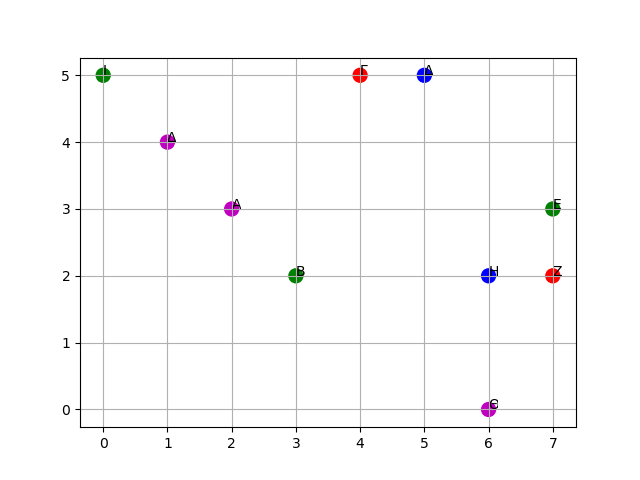
\includegraphics{graph1.png}
\end{figure}
\begin{exercise}
\sel[2]{89}
Σε ορθοκανονικό σύστημα ημιαξόνων να τοποθετήσεις τα σημεία Α(2,1), Β(1,2), Γ(2,3)
και Δ(3,2). Τι σχήμα είναι το ΑΒΓΔ; Αν τα ευθύγραμμα τμήματα ΑΓ και ΒΔ τέμνονται
στο σημείο Κ, ποιες είναι οι συντεταγμένες του Κ;
\end{exercise}
\begin{lstlisting}
import matplotlib.pyplot as plt

plt.clf()
points = [(2,1), (1,2), (2,3), (3,2)]
pointName = ['Α','Β','Γ','Δ']
x = [p[0] for p in points]
y = [p[1] for p in points]
color=['m','g','r','b']
plt.grid()
plt.scatter(x,y, s=100 ,marker='o', c=color)
for (i,p) in enumerate(points):
    plt.annotate(pointName[i],(p[0],p[1]))

x = [points[0][0],points[2][0]]
y = [points[0][1],points[2][1]]
plt.plot(x,y)
x = [points[1][0],points[3][0]]
y = [points[3][1],points[3][1]]
plt.plot(x,y)

plt.show()
\end{lstlisting}
\begin{figure}
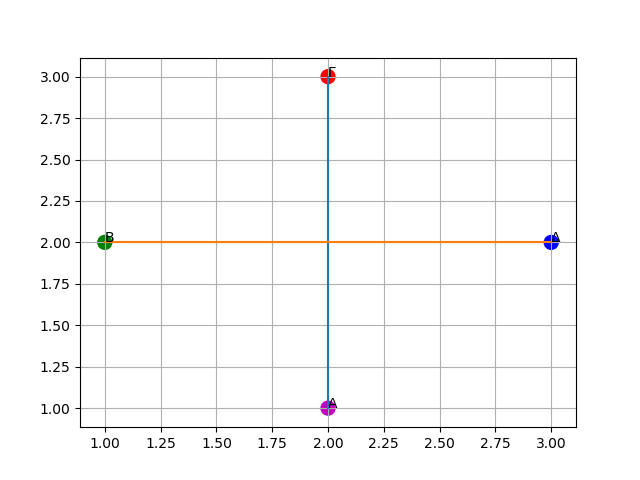
\includegraphics{graph2.png}
\end{figure}

\begin{exercise}
\sel[3]{89}
Γράψε πέντε διατεταγμένα ζεύγη σημείων, των οποίων η τετμημένη τους είναι ίση με
την τεταγμένη τους. Μπορείς να τα
τοποθετήσεις, σε ένα ορθοκανονικό
σύστημα ημιαξόνων; Τι παρατηρείς;
\end{exercise}
\begin{lstlisting}
import matplotlib.pyplot as plt

plt.clf()
points = [(1,1), (2,2), (5,5), (10,10), (15,15)]
pointName = ['Α','Β','Γ','Δ','Ε']
x = [p[0] for p in points]
y = [p[1] for p in points]
color=['m','g','r','b']
plt.grid()
plt.scatter(x,y, s=100 ,marker='o', c=color)
for (i,p) in enumerate(points):
    plt.annotate(pointName[i],(p[0],p[1]))

plt.show()
\end{lstlisting}
\begin{figure}
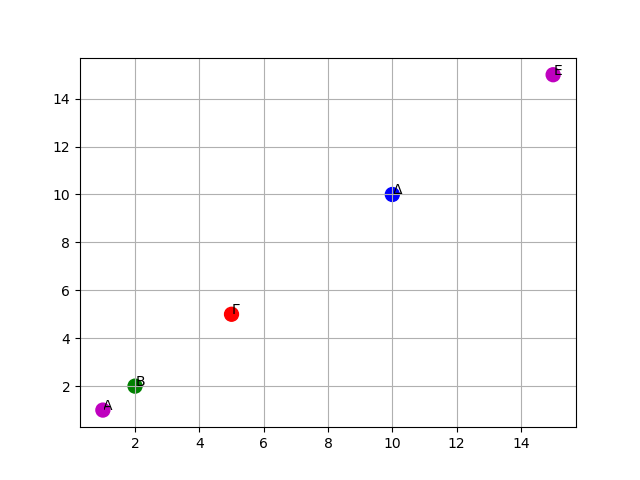
\includegraphics{graph3.png}
\end{figure}

\begin{exercise}
\sel{90}
Συμπλήρωσε τον παρακάτω πίνακα:
\begin{table}
\begin{tabular}{|l|c|c|c|}
Πλευρά τετραγώνου& 1,5 cm& 4 cm& 4,5 cm\\\hline
Περίμετρος τετραγώνου&&&\\\hline
\end{tabular}
\end{table}
\begin{itemize}
\item Εξήγησε πώς προκύπτουν οι αριθμοί της δεύτερης σειράς.
\item Βρες για κάθε τετράγωνο το κλάσμα πλευρά προς περίμετρο.
\item Ποιο είναι το συμπέρασμα που βγάζεις;
\end{itemize}
\end{exercise}
\begin{lstlisting}
>>> 4*1.5
6.0
>>> 4*4
16
>>> 4*4.5
18.0
\end{lstlisting}
\begin{tabular}{|l|c|c|c|}
Πλευρά τετραγώνου& 1,5 cm& 4 cm& 4,5 cm\\\hline
Περίμετρος τετραγώνου&6&16&18\\\hline
\end{tabular}
Θυμηθείτε το ποσοστό σε κλάσμα:
\begin{lstlisting}
def posostoseklasma(fx):
    fx = float(fx)
    denom = 100
    while int(fx) != fx:
         fx *= 10
         denom *= 10
    fx = int(fx)
    return(Fraction(fx,denom))
\end{lstlisting}
Το fx είναι είναι ο αριθμητής ενός κλάσματος με παρονομαστή 100. Εδώ δεν θα υπάρχει ο παρονομαστής 100 οπότε έχουμε denom = 1.
\begin{lstlisting}
def dekadikosseklasma(fx):
    fx = float(fx)
    denom = 1
    while int(fx) != fx:
         fx *= 10
         denom *= 10
    fx = int(fx)
    return(Fraction(fx,denom))

dekadikosseklasma(1.5/6)
dekadikosseklasma(4/16)
dekadikosseklasma(4.5/18)
\end{lstlisting}
και το αποτέλεσμα είναι:
\begin{lstlisting}
>>> dekadikosseklasma(1.5/6)
Fraction(1, 4)
>>> dekadikosseklasma(4/16)
Fraction(1, 4)
>>> dekadikosseklasma(4.5/18)
Fraction(1, 4)
\end{lstlisting}
Άρα παντού το κλάσμα είναι $\frac{1}{4}$.
\begin{exercise}
\sel{90}
Χρησιμοποιούμε τη φωτογραφική μηχανή
για να απεικονίσουμε εικόνες αντικειμένων. Οι εικόνες αυτές δείχνουν τα
πραγματικά αντικείμενα σε σμίκρυνση.
Στη φωτογραφία το ύψος ενός παιδιού
είναι 2 cm ενώ γνωρίζουμε ότι το πραγματικό του ύψος είναι 1,65 m = 165 cm. Πόση θα είναι τότε η σμίκρυνσή του
στη φωτογραφία;
\end{exercise}
\begin{lstlisting}
>>> 2/165
0.012121212121212121
\end{lstlisting}

\begin{exercise}
\sel{91}
Μετρούμε μια απόσταση, σε χάρτη, με κλίμακα 1:10.000.000 και τη βρίσκουμε
ίση με 2,4 cm. Ποια είναι η πραγματική απόσταση των δύο σημείων;
\end{exercise}
\begin{lstlisting}
>>> x = 2.4*10000000
>>> x
24000000
>>> x = x/100
>>> x
240000
>>> x = x/1000
>>> x
240
\end{lstlisting}
240Km
\begin{exercise}
\sel[3]{92}
Σε μια φωτογραφία το ύψος ενός ανθρώπου είναι 4 cm, ενώ το
πραγματικό το ύψος είναι 1,76 m. Πόσο έχει σμικρυνθεί η εικόνα του
ανθρώπου στη φωτογραφία;
\end{exercise}
\begin{lstlisting}
def pososto(x):
    print(str(round(x*100,2))+'%')
\end{lstlisting}
Αν θυμηθούμε τη συνάρτηση pososto τότε
\begin{lstlisting}
>>> pososto(4/176)
2.27%
\end{lstlisting}
\begin{exercise}
\sel[4]{92}Ένας προβολέας διαφανειών προβάλλει το κείμενο μιας διαφάνειας στον απέναντι
τοίχο. Αν ένα ``A'' έχει ύψος 7 mm στη διαφάνεια και 4,2 cm στον τοίχο, ποια είναι η
μεγέθυνση που δίνει ο προβολέας
\end{exercise}
\begin{lstlisting}
>>> pososto(4.2/0.7)
600%
\end{lstlisting}
\begin{exercise}
\sel[5]{92}
Η σύνθεση μιας μπλούζας είναι 80\% βαμβάκι και το υπόλοιπο πολυεστέρας. Aν η μπλούζα
ζυγίζει 820 gr, πόσα γραμμάρια ζυγίζουν τα νήματα του πολυεστέρα που περιέχει;
\end{exercise}
\begin{lstlisting}
>>> 820*20/100
164.0
\end{lstlisting}
\begin{exercise}
\sel[6]{92}
Να συμπληρωθεί ο πίνακας
\begin{table}
\begin{tabular}{|c|c|c|c|c|c|}
\hline
Κλίμακα&1:5&3:8&1:30&&1:100\\\hline
Μήκος σε σχέδιο&4cm &&12cm&2cm&3,5cm\\\hline
Πραγματικό ύψος&&24m&&10m&\\\hline
\end{tabular}
\end{table}
\end{exercise}
\begin{lstlisting}
>>> from fractions import Fraction
>>> 5*4
20
>>> 3/8*24
9.0
>>> 12*30
360
>>> Fraction(2,1000)
Fraction(1, 500)
>>> 3.5*100
350
\end{lstlisting}
Άρα ο πίνακας γίνεται:
\begin{table}
\begin{tabular}{|c|c|c|c|c|c|}
\hline
Κλίμακα&1:5&3:8&1:30&1:500&1:100\\\hline
Μήκος σε σχέδιο&4cm &9cm&12cm&2cm&3,5cm\\\hline
Πραγματικό ύψος&20cm&24m&360cm&10m&350cm\\\hline
\end{tabular}
\end{table}
\begin{exercise}
\sel[7]{92}
Οι διαστάσεις ενός ορθογωνίου παραλληλογράμμου είναι $x+2$ και $x$.

(α) Να γράψεις τη σχέση που συνδέει την περίμετρο Π του ορθογωνίου με το x.

(β) Να συμπληρώσεις τον πίνακα:
\begin{table}
\begin{tabular}{|c|c|c|c|c|}
x&&2&&4\\\hline
Π&8&&16&\\\hline
\end{tabular}
\end{table}
\end{exercise}
α)
\begin{lstlisting}
>>> from sympy import *
>>> x = symbols('x')
>>> p = x+x+2+x+x+2
>>> p
4*x + 4
\end{lstlisting}
β)
\begin{lstlisting}
>>> solve(p-8)
[1]
>>> p.subs(x,2)
12
>>> solve(p-16)
[3]
>>> p.subs(x,4)
20
\end{lstlisting}
και ο πίνακας γίνεται:
\begin{table}
\begin{tabular}{|c|c|c|c|c|}
\hline
x&1 &2  &3  &4\\\hline
Π&8&12&16&20\\\hline
\end{tabular}
\end{table}
\begin{exercise}
\sel[8]{92}
Aν οι διαστάσεις ενός δωματίου, σε ένα σχέδιο με κλίμακα 1:250, είναι 3x5, οι
πραγματικές διαστάσεις του δωματίου θα είναι .....x..... .
\end{exercise}
\begin{lstlisting}
>>> 3*250
750
>>> 5*250
1250
\end{lstlisting}
Οπότε το δωμάτιο είναι 7,5m x 12,5m αν οι διαστάσεις ήταν σε cm.
\begin{exercise}
\sel[9]{92}
Αν ανακατέψουμε 2 κιλά κόκκινο χρώμα και 3 κιλά κίτρινο χρώμα,
φτιάχνουμε μια συγκεκριμένη απόχρωση του πορτοκαλί. Αν
ανακατέψεις 5 κιλά κόκκινο χρώμα και 6 κιλά κίτρινο, θα πάρεις
την ίδια απόχρωση; Δικαιολόγησε την απάντησή σου.
\end{exercise}
\begin{lstlisting}
>>> 3/2 == 6/5
False
\end{lstlisting}
Όχι δεν είναι η ίδια απόχρωση.
\begin{exercise}
\sel[2]{93} Όταν ο Κώστας έκλεισε τα δώδεκα χρόνια είχε το ένα τρίτο της
ηλικίας της μητέρας του. Όταν θα γίνει είκοσι χρόνων, ο λόγος των
δύο ηλικιών τους θα παραμείνει ο ίδιος;
\end{exercise}
\begin{lstlisting}
>>> ilikiaMiteras = 3*12
>>> ilikiaMiteras
36
>>> xronia = 20-12
>>> xronia
8
>>> neailikiaMiteras = ilikiaMiteras + xronia
>>> neailikiaMiteras = 44
>>> 44/20 == 36/12
False
\end{lstlisting}
Άρα όχι.
\begin{exercise}
Να συμπληρωθεί ο πίνακας, αν γνωρίζουμε ότι τα ποσά x και 􀁜 είναι ανάλογα, με
συντελεστή αναλογίας $\alpha = \frac{2}{3}$.
\begin{table}
\begin{tabular}{|c|c|c|c|c|c|c}
\hline
x &0 &1 &0,3& &\\\hline
y &    &  &       & $\frac{5}{3}$ & 3\\\hline
\end{tabular}
\end{table}
\end{exercise}
$$
y = \frac{2}{3}x
$$
\begin{lstlisting}
>>> from sympy import *
>>> (x,y) = symbols('x y')
>>> e = 2/3*x
>>> e.subs(x,0)
0
>>> e.subs(x,1)
0.666666666666667
>>> e.subs(x,0.3)
0.200000000000000
>>> solve(e-5/3)
[2.50000000000000]
>>> solve(e-3)
[4.50000000000000]
\end{lstlisting}
Και ο πίνακας γίνεται:
\begin{table}
\begin{tabular}{|c|c|c|c|c|c|c}
\hline
x &0 &1 &0,3& 2,5&4,5\\\hline
y & 0   & 0,6666 & 0,2      & $\frac{5}{3}$ & 3\\\hline
\end{tabular}
\end{table}
\begin{exercise}
\sel[2]{92}
Σε ένα διάλυμα ζάχαρης η περιεκτικότητα σε ζάχαρη είναι 23\%. Πόσα γραμμάρια
ζάχαρης υπάρχουν σε 300 gr διαλύματος;
\end{exercise}
\begin{lstlisting}
>>> 300*23/100
69.0
\end{lstlisting}
\begin{exercise}
\sel[3]{97}
Ένα πλοίο έχει σταθερή ταχύτητα και καλύπτει απόσταση 80 Km σε 2 ώρες. Σε πόσο
χρόνο θα καλύψει απόσταση 2.000 Km;
\end{exercise}
$$\frac{2}{80}=\frac{x}{2000}$$
\begin{lstlisting}
>>> from sympy import *
>>> x = symbols('x')
>>> solve(2/80-x/2000)
[50.0000000000000]
\end{lstlisting}
Η απάντηση είναι 50 ώρες.
\begin{exercise}
Εξέτασε αν τα ποσά που δίνονται στους παρακάτω πίνακες είναι ανάλογα:
(α) 
\begin{table}
\begin{tabular}{|c|c|c|c|}
\hline
x&3&5 &7\\\hline
y&8&10&12\\\hline
\end{tabular}
\end{table}
(β)
\begin{table}
\begin{tabular}{|c|c|c|c|c|}
\hline
x&3&4 &6&11\\\hline
y&0,9&1,2&1,8&3,3\\\hline
\end{tabular}
\end{table}
\end{exercise}
\begin{lstlisting}
>>> 8/3==10/5==12/7
False
>>> 0.9/3==1.2/4==1.8/6==3.3/11
True
\end{lstlisting}
\begin{exercise}
\sel[4]{98}
Στον πίνακα που ακολουθεί, τα ποσά x και y είναι ανάλογα. Υπολόγισε τον συντελεστή
αναλογίας τους και συμπλήρωσε τον πίνακα.
\begin{table}
\begin{tabular}{|c|c|c|c|c|c|c|c|c|}
x& 5& 0& 1& & & 3,7& 0,61&\\\hline
y&10,05& & &2 &0,125&&& 0,55\\hline
\end{tabular}
\end{table}
\end{exercise}
Η αναλογία είναι 
\begin{lstlisting}
>>> 10.05/5
2.0100000000000002
\end{lstlisting}
Όμως αυτό είναι 2,01
Οπότε:
\begin{lstlisting}
>>> 0*2.01
0.0
>>> 1*2.01
2.01
>>> 2/2.01
0.9950248756218907
>>> 0.125/2.01
0.06218905472636817
>>> 3.7*2.01
7.436999999999999
>>> 0.61*2.01
1.2260999999999997
>>> 0.55/2.01
0.27363184079601993
\end{lstlisting}
και προσεγγιστικά ο πίνακας γίνεται:
\begin{table}
\begin{tabular}{|c|c|c|c|c|c|c|c|c|}
x& 5       & 0& 1      &0,995 & 0,0622 & 3,7   & 0,61&  0,273632\\\hline
y&10,05& 0 & 2.01&2         &0,125      &7,437& 1.226&0,55\\hline
\end{tabular}
\end{table}

\section{Ανάλογα ποσά}
\begin{exercise}
Σε	μια	παρέα	κάποιος	υποστήριζε	ότι	το	βάρος	του	ανθρώπου	είναι	ανάλογο	του	ύψους	του. Μετρήθηκαν,	λοιπόν,	όλοι	και	έβαλαν	στον	παρακάτω	πίνακα	τα	αποτελέσματα σε Κ.
\begin{table}
\begin{tabular}{|c|c|c|c|c|}
\hline
Βάρος& 58& 71& 56& 68\\\hline
Ύψος & 1,60&1,65&1,62&1,72\\\hline
\end{tabular}
\end{table}
\begin{itemize}
\item Μπορείς	να	επιβεβαιώσεις	ή	να	απορρίψεις	τον		ισχυρισμό	αυτό;		
\item Πώς	δικαιολογείς	το	συμπέρασμά	σου;
\end{itemize}
\end{exercise}
\begin{lstlisting}
>>> 58/1.60 == 71/1.65
False
\end{lstlisting}
Οπότε ο ισχυρισμός απορρίπτεται.
\begin{exercise}
O	μανάβης	πουλάει	τα	καρπούζια	προς	0,4	Q
	το	κιλό.	Μέσα	σε	μια	ημέρα	πούλησε	11	καρπούζια	που	ζύγιζαν	100	κιλά	συνολικά.	Ο	μανάβης	έγραφε,	σ’	ένα	χαρτί,	τα	λεφτά	που	 εισέπραττε	κάθε	φορά.	Ξέχασε,	όμως,	μία	φορά	να	το	σημειώσει.

→		Μπορείς	να	τον	βοηθήσεις	συμπληρώνοντας 	τα	κενά	του	παρακάτω	πίνακα: 
\begin{table}
\begin{tabular}{|c|c|c|c|c|c|c|c|c|c|c|c|}
\hline
Tιμή& 6€ & 2,8€ & 5,2€ & 3,2€ & & 3,6€ & 4,8€ & 2,4€ & 1,6€ & 4,4€ & 2€\\\hline
Κιλά&       &         &          &         &&            &          &          &        &            &     \\\hline
\end{tabular}
\end{table}    
\begin{itemize}
 \item Δικαιολόγησε τα	αποτελέσματα	των	πράξεων	που 	έκανες	και	προσπάθησε	να		διατυπώσεις	έναν	γενικό	κανόνα. 
\end{itemize}

 \end{exercise}
 Τα χρήματα που πήρε συνολικά θα είναι $0,4*100=40$€. Οπότε μπορούμε να αθροίσουμε τα χρήματα και να βρούμε τα κιλά που πωλήθηκαν από τα χρήματα.
 \begin{lstlisting}
 >>> 6+2.8+5.2+3.2+3.6+4.8+2.4+1.6+4.4+2
36.0
>>> 36/0.4
90.0
>>> 100-90
10
>>> 10*0.4
4.0
\end{lstlisting}
Για να συμπληρώσουμε ολόκληρο τον πίνακα μπορούμε να βρούμε τα κιλά από τα χρήματα διαιρώντας με το 0,4.
\begin{lstlisting}
>>> 6/0.4
15.0
>>> 2.8/0.4
6.999999999999999
>>> 5.2/0.4
13.0
>>> 3.6/0.4
9.0
>>> 4.8/0.4
11.999999999999998
>>> 2.4/0.4
5.999999999999999
>>> 1.6/0.4
4.0
>>> 4.4/0.4
11.0
>>> 2/0.4
5.0
>>>
\end{lstlisting}
Αν λάβουμε υπόψη τις στρογγυλοποιήσεις ο πίνακας γίνεται:
\begin{table}
\begin{tabular}{|c|c|c|c|c|c|c|c|c|c|c|c|}
\hline
Tιμή& 6€ & 2,8€ & 5,2€ & 3,2€ & 4€ & 3,6€ & 4,8€ & 2,4€ & 1,6€ & 4,4€ & 2€\\\hline
Κιλά&  15 &  7    &   13    &   8      & 10& 9      &  12    &   6     &  4    &   1       &  5   \\\hline
\end{tabular}
\end{table}    
\begin{exercise}
\sel{99}
Η	σχέση,	μεταξύ	δύο	ανάλογων	ποσών	x	και		με	συντελεστή	αναλογίας	α	=	3,	δίνεται	από	τον	τύπο:		
$$ y =	3 \cdot x$$.
\begin{itemize}
\item Συμπλήρωσε	τα	κενά	του	πίνακα	και	με	άλλες	τιμές	των	αναλόγων	ποσών	x	και	.
\item Βρες	τα	σημεία	του	επιπέδου	που		αναπαριστούν	τα	παραπάνω		ζεύγη	τιμών.
\item Προσπάθησε	να	διαπιστώσεις,	εάν		τα	σημεία	ανήκουν	σε	μία	ημιευθεία		ή	όχι.	
\item Η	ημιευθεία	αυτή	περνάει	από		το	σημείο	Ο(0,0)	δηλαδή	την	αρχή		των	ημιαξόνων;
\end{itemize}
\end{exercise}
\begin{lstlisting}
import matplotlib.pyplot as plt
from random import randint
from math import floor
plt.clf()
points = []
for i in range(10):
    x = 0+randint(0,10)*0.5
    y = 3*x
    points.append((x,y))

x = [p[0] for p in points]
y = [p[1] for p in points]
color=['m','g','r','b']
plt.grid()
plt.scatter(x,y, s=100 ,marker='o', c=color)

plt.show()
\end{lstlisting}
\begin{figure}
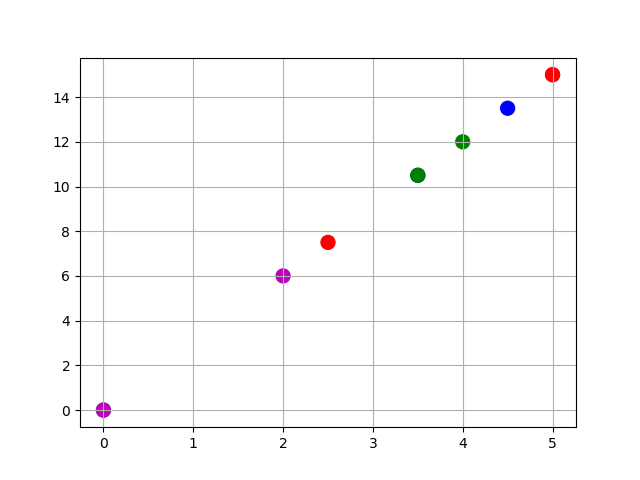
\includegraphics{3x.png}
\end{figure}
Οπότε τα σημεία ανήκουν σε ημιευθεία η οποία περνάει από την αρχή των αξόνων.

\begin{exercise}
\sel{100}
Δίνονται	οι	 πίνακες	Α,	Β,	 Γ	και	Δ.	

(α)	Να	γίνει	η	γραφική	απεικόνιση	των	ζευγών	(x,y)	των	πινάκων	στο επίπεδο	και	
(β)	να	διαπιστωθεί	σε	ποια	περίπτωση	αυτά	παριστάνουν	ποσά	ανάλογα.   

\begin{table}
\begin{tabular}{|c|c|c|c|c|}
x&0&1&2&3\\
y&0&2&1&1.5\\
\end{tabular}
\caption{Πίνακας Α}
\end{table}

\begin{table}
\begin{tabular}{|c|c|c|c|c|}
x&0&1&2&3\\
y&1&1.5&2&2.5\\
\end{tabular}
\caption{Πίνακας B}
\end{table}

\begin{table}
\begin{tabular}{|c|c|c|c|c|}
x&0&1&2&3\\
y&0&1&2&3\\
\end{tabular}
\caption{Πίνακας Γ}
\end{table}


\begin{table}
\begin{tabular}{|c|c|c|c|c|}
x&0&1&2&3\\
y&0&0.5&1&1.5\\
\end{tabular}
\caption{Πίνακας Δ}
\end{table}
\end{exercise}
\begin{lstlisting}
import matplotlib.pyplot as plt

plt.clf()
pointsA = [(0,0),(1,2),(2,1),(3,1.5)]
pointsB = [(0,1),(1,1.5),(2,2),(3,2.5)]
pointsC = [(0,0),(1,1),(2,2),(3,3)]
pointsD = [(0,0),(1,0.5),(2,1),(3,1.5)]

x = [p[0] for p in pointsA]
y = [p[1] for p in pointsA]
plt.grid()
plt.plot(x,y, marker='o', c='r')


x = [p[0] for p in pointsB]
y = [p[1] for p in pointsB]
plt.grid()
plt.plot(x,y, marker='o', c='g')


x = [p[0] for p in pointsC]
y = [p[1] for p in pointsC]
plt.grid()
plt.plot(x,y,marker='o', c='b')


x = [p[0] for p in pointsD]
y = [p[1] for p in pointsD]
plt.grid()
plt.plot(x,y, marker='o', c='m')
plt.show()
\end{lstlisting}

\begin{figure}
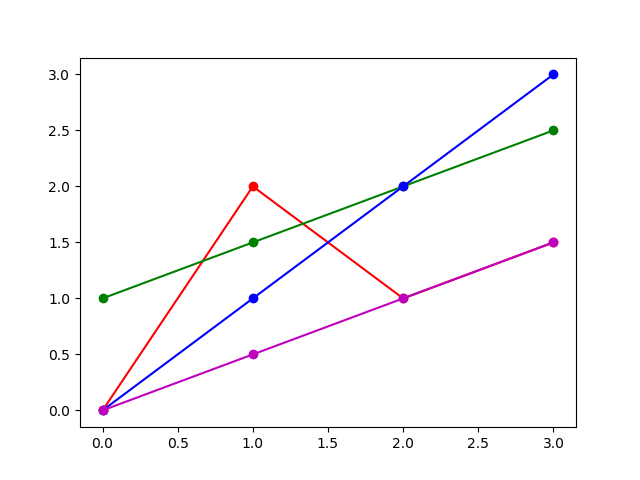
\includegraphics{4plots.png}
\end{figure}

Μια πιο σύντομη έκδοση του προγράμματος που δίνει το ίδιο αποτέλεσμα είναι:
\begin{lstlisting}
import matplotlib.pyplot as plt

plt.clf()
pointslist = [[(0,0),(1,2),(2,1),(3,1.5)],
          [(0,1),(1,1.5),(2,2),(3,2.5)],
          [(0,0),(1,1),(2,2),(3,3)],
          [(0,0),(1,0.5),(2,1),(3,1.5)]]
colors = ['r','g','b','m']
for (i,points) in enumerate(pointslist):
    x = [p[0] for p in points]
    y = [p[1] for p in points]
    plt.grid()
    plt.plot(x,y, marker='o', c=colors[i])

plt.show()
\end{lstlisting}

\begin{exercise}
\sel[1]{101}
Δύο  ποσά  x και  είναι ανάλογα, με συντελεστή αναλογίας α = 1,5. 

(α)	Δημιούργησε έναν πίνακα τιμών των δύο ποσών, ο οποίος να περιέχει  τουλάχιστον δύο  ζεύγη τιμών. 

(β) Βρες τα σημεία που αναπαριστούν τα ζεύγη τιμών του πίνακά σου. 

(γ)  Σχεδίασε τη γραφική παράσταση της σχέσης αναλογίας των ποσών x και , σε  ένα ορθοκανονικό σύστημα ημιαξόνων.
\end{exercise}
\begin{table}
\begin{tabular}{|c|c|c|}
\hline
x&1&2\\\hline
y&1.5&3\\\hline
\end{tabular}
\end{table}
\begin{lstlisting}
import matplotlib.pyplot as plt

plt.clf()
points = [(1,1.5),(2,3)]

x = [p[0] for p in points]
y = [p[1] for p in points]

plt.grid()
plt.plot(x,y, marker='o', c='r')

plt.show()
\end{lstlisting}
\begin{figure}
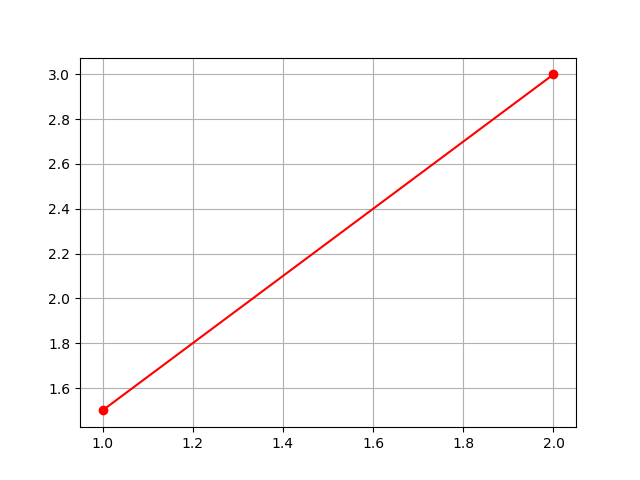
\includegraphics{sel101_1.png}
\end{figure}
Καλύτερα όμως είναι να βάλουμε και το σημείο (0,0) ως εξής:
\begin{lstlisting}
import matplotlib.pyplot as plt

plt.clf()
points = [(0,0),(1,1.5),(2,3)]

x = [p[0] for p in points]
y = [p[1] for p in points]

plt.grid()
plt.plot(x,y, marker='o', c='r')

plt.show()
\end{lstlisting}
\begin{figure}
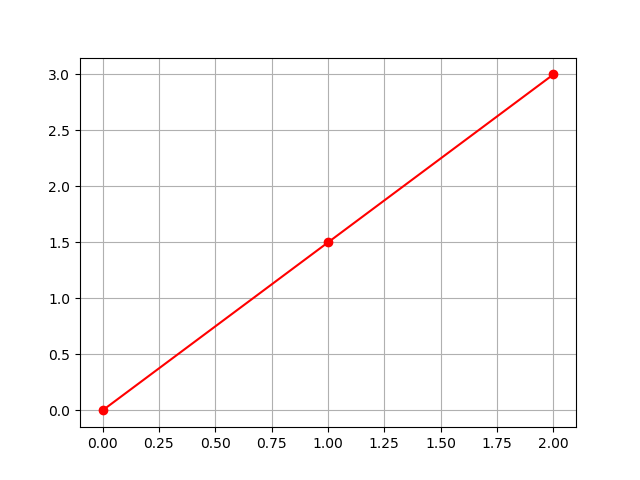
\includegraphics{sel101_1a.png}
\end{figure}

\begin{exercise}
\sel[2]{101}
Σε κατάλληλο ορθογώνιο σύστημα ημιαξόνων να σχεδιάσεις τις γραφικές παραστάσεις για κάθε μία από τις ακόλουθες σχέσεις αναλογίας: 

(α)	$y = \left(\frac{1}{2}\right)\cdot x$,	

(β)	$y = 3 \cdot x$,	

(γ)	$y =	5,5	\cdot x$

(δ)	$y =	10\cdot x$,	

(ε) $y  =	0,01 \cdot x$.
\end{exercise}

Μπορούμε να τις σχεδιάσουμε και όλες μαζί με διαφορετικά χρώματα. Έχουν ένα κοινό σημείο ενώ μπορούμε να υπολογίσουμε εύκολα ένα δεύτερο, π.χ. για $x=10$.
\begin{lstlisting}
import matplotlib.pyplot as plt
from sympy import *
x = symbols('x')

analogies = [1/2*x,3*x,5.5*x,10*x,0.01*x]
colors = ['r','g','b','c','m']
for (i,s) in enumerate(analogies):
    x = symbols('x')
    points = [(0,0),(10,s.subs(x,10))]
    x = [p[0] for p in points]
    y = [p[1] for p in points]
    plt.grid()
    plt.plot(x,y, marker='o', c=colors[i])

plt.show()
\end{lstlisting}
\begin{figure}
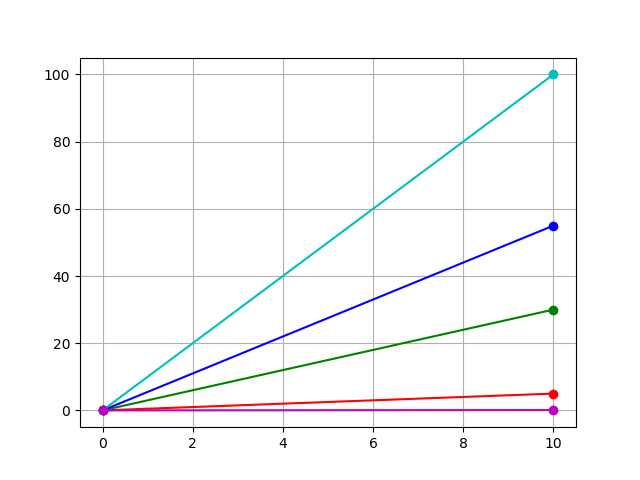
\includegraphics{sel101_2.png}
\end{figure}
Όμως τα συστήματα δεν είναι κατάλληλα για όλες τις γραφικές παραστάσεις ειδικά η τελευταία φαίνεται να είναι σταθερή στο 0. Αν τη σχεδιάσουμε μόνη της η matplotlib θα υπολογίσει ένα κατάλληλο σύστημα αξόνων.
\begin{lstlisting}
import matplotlib.pyplot as plt
from sympy import *

points = [(0,0),(10,0.01*10]
x = [p[0] for p in points]
y = [p[1] for p in points]
plt.grid()
plt.plot(x,y, marker='o', c='m')

plt.show()
\end{lstlisting}
\begin{figure}
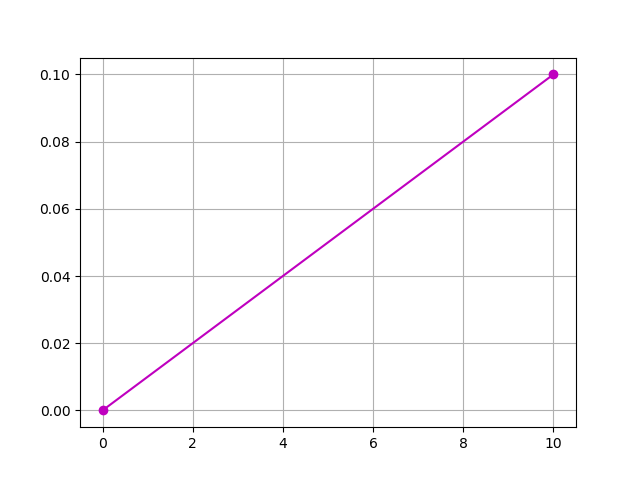
\includegraphics{sel101_2a.png}
\end{figure}

%\chapter{Θετικοί και αρνητικοί αριθμοί}
\section{Θετικοί και Αρνητικοί Αριθμοί (Ρητοί αριθμοί) -
H ευθεία των ρητών - Τετμημένη σημείου}
\begin{exercise}
\sel[4]{117} 
Στα ζεύγη αριθμών που ακολουθούν να βρεις ποιοι αριθμοί είναι ομόσημοι και ποιοι είναι ετερόσημοι: (α) 3 και +3, (β) 2 και 5, (γ) –2 και –4, (δ) 7 και +9, (ε) –2 και 1,(στ) 17 και –20, (ζ) –9 και –3,2, (η) –10,5 και 11, (θ) –3 και –100, (ι) +6,7 και +12,3
\end{exercise}

Αργότερα θα μάθεις έναν εύκολο τρόπο για να ελέγξεις αν δύο αριθμοί είναι ομόσημοι οι ετερόσημοι, με όσα έχεις δει μέχρι τώρα μπορείς να το κάνεις ως εξής:
\begin{lstlisting}
    while (True):
        a = float(input('α> '))
        b = float(input('β> '))

        if a > 0:
            if b > 0:
                print("Ομόσημοι")
            else:
                print("Ετερόσημοι")
        else:
            if b < 0:
                print("Ομόσημοι")
            else:
                print("Ετερόσημοι")
\end{lstlisting}
και το αποτέλεσμα θα είναι:
\begin{lstlisting}
α>3
β>+3
Ομόσημοι
α>2
β>5
Ομόσημοι
α>-2
β>-4
Ομόσημοι
α>7
β>+9
Ομόσημοι
α>-2
β>1
Ετερόσημοι
α>17
β>-20
Ετερόσημοι
α> -9
β> -3.2
Ομόσημοι
α> -10.5
β> 11
Ετερόσημοι
α> -3
β> -100
Ομόσημοι
α> 6.7
β> 12.3
Ομόσημοι
\end{lstlisting}

\begin{exercise}
\sel[6]{117} Βρες τη λέξη που σχηματίζεται από τα γράμματα με τετμημένες –6, 10, 9, –9, 5, –5, 0 στο παρακάτω σχήμα. Στη συνέχεια γράψε μ’ αυτό τον τρόπο ένα όνομα που σου αρέσει.
Εικόνα
\end{exercise}
Οι αντιστοιχίσεις μπορούν να αποθηκευτούν σε ένα λεξικό και να βρούμε τη λέξη ως εξής:
\begin{lstlisting}
antistoixiseis = {-11:'Ψ',
-10:'Φ',
-9:'T',
-8:'Ρ',
-7:'Ξ',
-6:'Μ',
-5:'Κ',
-4:'Θ',
-3:'Ζ',
-2:'Δ',
-1:'Β',
0:'Ο',
1:'Α',
2:'Γ',
3:'Ε',
4:'Η',
5:'Ι',
6:'Λ',
7:'Ν',
8:'Π',
9:'Σ',
10:'Υ',
11:'Χ',
12:'Ω'}
tetmimenes = [-6,10,9,-9,5,-5,0]
for i in tetmimenes:
    print(antistoixiseis[i])
\end{lstlisting}

Το αποτέλεσμα θα είναι:
\begin{lstlisting}
Μ
Υ
Σ
T
Ι
Κ
Ο
\end{lstlisting}
Αν αλλάξουμε την εντολή print ως εξής:
\begin{lstlisting}
print(antistoixiseis[i],end='')
\end{lstlisting}
Θα προκύψει:
\begin{lstlisting}
ΜΥΣΤΙΚΟ
\end{lstlisting}
Με το end='' δίνουμε την οδηγία στην Python να μην αλλάζει γραμμή μετά από κάθε print.
H κωδικοποίηση γίνεται με το ίδιο λεξικό αλλά ως εξής:
\begin{lstlisting}
lexi = 'ΜΗΝΥΜΑ'
for l in lexi:
    print(list(antistoixiseis.keys())[
        list(antistoixiseis.values()).index(l)],
          end=',')
\end{lstlisting}
Ο λόγος για τον οποίο είναι τόσο πολύπλοκη η κωδικοποίηση είναι ότι το λεξικό δεν μπορεί να υποστηρίξει και τις δύο κατευθύνσεις πρόσβασης. Ένας εναλλακτικός τρόπος αναπαράστασης των ίδιων δεδομένων θα ήταν ο εξής:
\begin{lstlisting}
grammata = ['Ψ','Φ','T','Ρ','Ξ','Μ','Κ','Θ','Ζ','Δ','Β','Ο','Α','Γ','Ε','Η','Ι','Λ','Ν','Π','Σ','Υ','Χ','Ω']
arithmoi = [-11,-10,-9,-8,-7,-6,-5,-4,-3,-2,-1,0,1,2,3,4,5,6,7,8,9,10,11,12]

tetmimenes = [-6,10,9,-9,5,-5,0]
for i in tetmimenes:
    print(grammata[arithmoi.index(i)],end='')
print()

lexi = 'ΜΗΝΥΜΑ'
for l in lexi:
    print(arithmoi[grammata.index(l)],end=',')
\end{lstlisting}
που δίνει το σωστό αποτέλεσμα:
\begin{lstlisting}
ΜΥΣTΙΚΟ
-6,4,7,10,-6,1,
\end{lstlisting}
\begin{exercise}
\sel[7]{117}
Τα σημεία Α και Β έχουν τετμημένες α και β, αντίστοιχα. Να βρεθεί η τετμημένη του μέσου Μ του τμήματος ΑΒ όταν: (α) α = +5 και β = +8, (β) α = –4 και β = –13.
\end{exercise}
\begin{lstlisting}
>>> (5+8)/2
6.5
>>> (-4+(-13))/2
-8.5
\end{lstlisting}
\section{Απόλυτη τιμή}
Να συμπληρώσεις τον πίνακα που ακολουθεί:
\begin{table}[h]
\begin{tabular}{|c|c|c|c|c|c|c|}
\hline
Αριθμός& -2,73 & +7,66 & -1,05 & 0,+8,07 & -8\\\hline
Aπόσταση του σημείου που αντιστοιχεί από την αρχή του άξονα &&&&&\\\hline
\end{tabular}
\end{table}

Γνωρίζουμε ότι η απόσταση από την αρχή του άξονα είναι η απόλυτη τιμή. Η python μπορεί να υπολογίσει την απόλυτη τιμή με την ειδική εντολή abs, τα τρία πρώτα γράμματα της λέξης absolute.
Οπότε έχουμε:
\begin{lstlisting}
>>> abs(-2.73)
2.74
>>> abs(+7.66)
7.66
>>> abs(-1.05)
1.05
>>> abs(0)
0
>>> abs(+8.07)
8.07
>>> abs(-8)
8
\end{lstlisting}
\begin{exercise}
\sel[3]{121}
ΣΩΣΤΟ ή  ΛΑΘΟΣ
(α) Iσχύει η ανισότητα: $–5,7 < 5,7$. 

(β) Ισχύει η ανισότητα: $–7,6 > –6,7$. 

(γ) Στην ανισότητα $2,3 < x < 4,7$ ο x μπορεί να πάρει 2 ακέραιες τιμές. 

(δ) Υπάρχουν 5 ακριβώς ακέραιοι που αληθεύουν τη σχέση: $–2 \leq x \leq 2$.

(ε) Δύο ακέραιοι με αντίθετο πρόσημο είναι αντίθετοι.
\end{exercise}
(α)
\begin{lstlisting}
>>> -5.7 < 5.7
True
\end{lstlisting}
Σωστό
(β)
\begin{lstlisting}
>>> -7.6 > -6.7
False
\end{lstlisting}
Λάθος
(γ) 
\begin{lstlisting}
for i in range(10):
    if i > 2.3 and i < 4.7:
        print(i)
\end{lstlisting}
το αποτέλεσμα είναι:
\begin{lstlisting}
3
4
\end{lstlisting}
Ο x μπορεί να πάρει 2 ακέραιες τιμές άρα ΣΩΣΤΟ.
(δ)
\begin{lstlisting}
for i in range(-3,3):
    if i >= -2 and i <= 2:
        print(i)
\end{lstlisting}
το αποτέλεσμα είναι:
\begin{lstlisting}
-2
-1
0
1
2
\end{lstlisting}
Υπάρχουν 5 ακριβώς ακέραιοι που αληθεύουν τη σχέση άρα ΣΩΣΤΟ
(ε) Λάθος γιατί υπάρχει η εξαίρεση του μηδενός.

\begin{exercise}
\sel[4]{121} Βρες την απόλυτη τιμή των ρητών: (α) +7,25, (β) –2,5, (γ) +16, (δ) –20,05, (ε) –58.
\end{exercise}
\begin{lstlisting}
>>> abs(+7.25)
7.25
>>> abs(-2.5)
2.5
>>> abs(+16)
16
>>> abs(-20.05)
20.05
>>> abs(-58)
58
\end{lstlisting}
\begin{exercise}
\sel[5]{121}Βρες τους αριθμούς που έχουν ως απόλυτη τιμή: (α) 100, (β) 21,7, (γ) 0, (δ) 7,03, (ε) 5,2.
\end{exercise}
\begin{lstlisting}
def fromabs(x):
    if x == 0:
        return(0)
    else:
        return((x, -x))

>>> fromabs(100)
(100, -100)
>>> fromabs(21.7)
(21.7, -21.7)
>>> fromabs(0)
0
>>> fromabs(7.03)
(7.03, -7.03)
>>> fromabs(5.2)
(5.2, -5.2)
\end{lstlisting}
\begin{exercise}
\sel[6]{121}
Συμπλήρωσε τον πίνακα:
\begin{table}[h]
\begin{tabular}{|c|c|c|c|c|c|c|c|c|}
\hline
Αριθμός      &1&           &         &-19&   &    & & \\\hline
Αντίθετος    & &           &         &   & -8& 12 & & \\\hline
Απόλυτη τιμή & &\multicolumn{2}{c}{2}&   &   &    &\multicolumn{2}{c}{7}\\\hline
\end{tabular}
\end{table}
\end{exercise}
Μπορούμε να χρησιμοποιήσουμε την abs και την fromabs για να βρούμε κάποια στοιχεία του πίνακα ο οποίος διαρμορφώνεται ως εξής:
\begin{table}[h]
\begin{tabular}{|c|c|c|c|c|c|c|c|c|}
\hline
Αριθμός      &1 &   2       &    -2   &-19& 8 & -12& 7&-7\\\hline
Αντίθετος    &-1&  -2       &     2   &19 & -8& 12 &-7& 7\\\hline
Απόλυτη τιμή &1 &\multicolumn{2}{c}{2}& 19& 8 & 12 &\multicolumn{2}{c}{7}\\\hline
\end{tabular}
\end{table}

\begin{exercise}
\sel[7]{121}Toποθέτησε στον άξονα $x'Οx$ τα σημεία με τετμημένες:$–9$, $–5,5$, $+8$, $-3$, $-7,25$, $+1$, $+12$, $+3$, $+9$. 
Ποια από αυτά είναι συμμετρικά ως προς την αρχή του άξονα;
\end{exercise}
\begin{lstlisting}
import matplotlib.pyplot as plt

plt.clf()
points = [(-9,0), (-5.5,0), (8,0), (-3,0), (-7.25,0), (+1,0), (+12,0), (+3,0), (+9,0)]
pointName = ['Α','Β','Γ','Δ','Ε','Ζ','Η','Θ','Ι']
x = [p[0] for p in points]
y = [p[1] for p in points]
plt.grid()
plt.scatter(x,y, s=100 ,marker='o')
for (i,p) in enumerate(points):
    plt.annotate(pointName[i],(p[0],p[1]))

plt.show()
\end{lstlisting}
Που δίνει το αποτέλεσμα:
\begin{figure}[h]
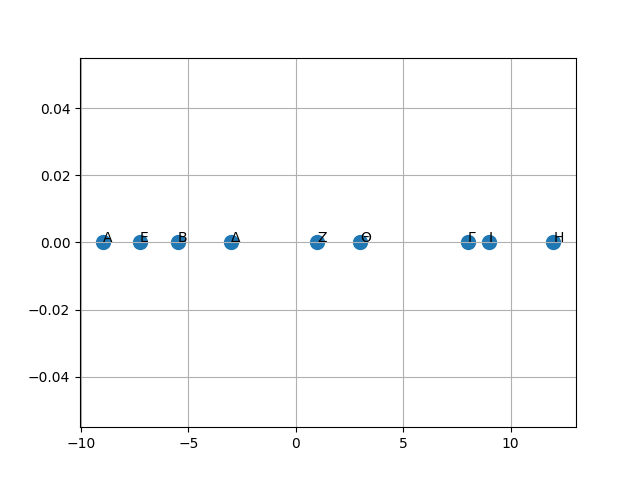
\includegraphics{graph10.png}
\end{figure}
Για να δούμε ποια είναι συμμετρικά θα πρέπει να δούμε ποια ζευγάρια έχουν τις ίδιες απόλυτες τιμές:
\begin{lstlisting}
    l = [-9, -5.5, 8, -3, -7.25, +1, +12, +3, +9]
    for i in l:
        apTimi = abs(i)
        for j in l:
            if apTimi == abs(j) and i != j:
                print(i,j)
\end{lstlisting}
Που δίνει το αποτέλεσμα:
\begin{lstlisting}
-9 9
-3 3
3 -3
9 -9
\end{lstlisting}
\begin{exercise}
\sel[8]{121}
Σχεδίασε τον άξονα $x'Ox$, με κατάλληλη μονάδα για να παραστήσεις τα σημεία με
τετμημένες τους αριθμούς: $–20,5$, $+15$, $–39,75$, $–68,25$, $+70$, $+52,25$,$+43$, $–69$.
\end{exercise}
\begin{lstlisting}
import matplotlib.pyplot as plt

plt.clf()
points = [(-20.5,0), (+15,0), (-39.75,0), (-68.25,0), (+70,0), (+52.25,0), (+43,0), (-69,0)]
pointName = ['Α','Β','Γ','Δ','Ε','Ζ','Η','Θ']
x = [p[0] for p in points]
y = [p[1] for p in points]
plt.grid()
plt.scatter(x,y, s=100 ,marker='o')
for (i,p) in enumerate(points):
    plt.annotate(pointName[i],(p[0],p[1]))

plt.show()
\end{lstlisting}
Που δίνει το αποτέλεσμα:
\begin{figure}[h]
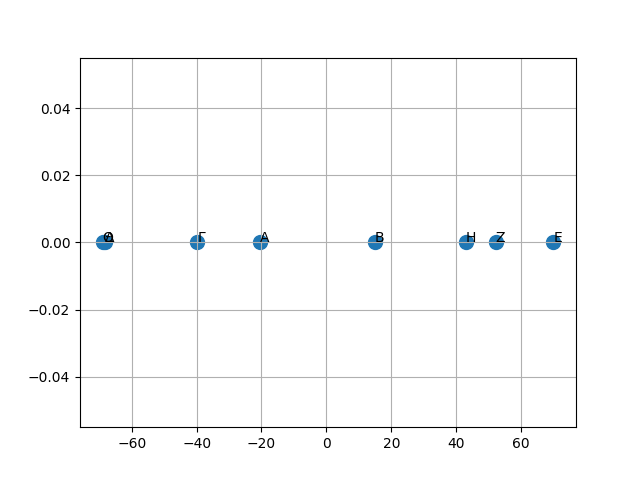
\includegraphics{graph11.png}
\end{figure}
Έτσι βλέπουμε ότι η python επέλεξε μια μονάδα να αντιστοιχεί στο 20 (1:20) και σε αυτή τη κλίμακα είναι αδύνατο να διακρίνουμε τους αριθμούς $-69$ και $-68,25$.
\begin{exercise}
Να συγκρίνεις τους αριθμούς: (α) +41 και +38, (β) 9 και 11, (γ) –3 και –2, (δ) –9 και –16, (ε) 7 και –8, (στ) 0 και –3, (ζ) 0 και +4.
\end{exercise}
\begin{lstlisting}
>>> 41 > 38
True
>>> 9 < 11
True
>>> -3 < -2
True
>>> -9 > -16
True
>>> 7 > -8
True
>>> 0 > -3
True
>>> 4 > 0
True
\end{lstlisting}
\begin{exercise}
\sel[10]{121}
Να συγκρίνεις τους αριθμούς: (α) $11$, $–11$ και $|11|$, (β) $–3$, $+3$ και $|3|$. Τι συμπεραίνεις;
\end{exercise}
\begin{lstlisting}
>>> 11 == abs(11)
True
>>> -11 < abs(11)
True
>>> -3 < abs(3)
True
>>> 3 == abs(3)
True
\end{lstlisting}
\begin{exercise}
\sel[11]{121}
Να γράψεις τους αριθμούς: –2, +7, +15, –3, 0, –4, +5, –8 και –10 σε αύξουσα σειρά.
\end{exercise}
\begin{lstlisting}
>>> print(sorted([-2, +7, +15, -3, 0, -4, +5, -8, -10]))
[-10, -8, -4, -3, -2, 0, 5, 7, 15]
\end{lstlisting}
\begin{exercise}
\sel[12]{121}
Να συμπληρώσεις με το κατάλληλο σύμβολο: <, > ή = τα κενά, ώστε να προκύψουν
αληθείς σχέσεις: (α) $–3 \ldots –8$, (β) $–4 \ldots 10$, (γ) $0 \ldots –1$, (δ) $+3 \ldots 0$, (ε) $–5 \ldots –|–5|$,
(στ) $–5 \ldots –(+5)$, (ζ) $|+7| \ldots |–7|$, (η) $–(–8) \ldots –8$, (θ) $+3 \ldots –(+4)$, (ι) $0 \ldots –|–4|$.
\end{exercise}
\begin{lstlisting}
>>> -3 > -8
True
>>> -4 < 10
True
>>> 0 > -1
True
>>> 3 > 0
True
>>> -5 == -abs(-5)
True
>>> -5 == -(+5)
True
>>> abs(+7) == abs(-7)
True
>>> -(-8) > -8
True
>>> 3 > -(+4)
True
>>> 0 > -abs(-4)
True
\end{lstlisting}

\begin{exercise}
Το x παριστάνει έναν ακέραιο αριθμό. Για ποιες τιμές του x θα ισχύουν οι σχέσεις:
(α) $–13 < x < –8$, (β) $–4 > x > –5$, (γ) $–2 < x < 5$.
\end{exercise}
\begin{lstlisting}
>>> for i in range(-14,-7):
    if i > -13 and i < -8:
        print(i) 
-12
-11
-10
-9
>>> for i in range(-6,0):
    if i < -4 and i > -5:
        print(i) 

>>> for i in range(-3,6):
    if i>-2 and i<5:
        print(i)
-1
0
1
2
3
4
\end{lstlisting}
\section{Πρόσθεση ρητών αριθμών}
\begin{exercise}
\sel[1]{123}
Σε μια πόλη παρατηρήθηκαν οι παρακάτω αυξομειώσεις της θερμοκρασίας:
Αρχικές θερμοκρασίες Αυξομειώσεις θερμοκρασίας

(α) Βράδυ +1°C την επόμενη μέρα αυξήθηκε κατά 4°C

(β) Μεσημέρι –1°C το βράδυ μειώθηκε κατά 2°C

(γ) Βράδυ –2°C την επόμενη μέρα αυξήθηκε κατά 5°C

(δ) Μεσημέρι +5°C το βράδυ μειώθηκε κατά 7°C

(ε) Μεσημέρι –3°C το βράδυ μειώθηκε κατά 3°C
\end{exercise}
\begin{lstlisting}
>>> 1 + 4
5
>>> -1 + (-2)
-3
>>> -2 + 5
3
>>> 5 + (-7)
-2
>>> +3 + (-3)
0
\end{lstlisting}
\begin{exercise}
\sel[2]{124}
Να υπολογιστούν τα παρακάτω αθροίσματα:
(α) $(+5,6) + (+8,7) + (-3,2) + (-6,9) + (+3,2) + (-7,4)$ και
(β) $(-1,8) + (+4,8) + (+9,7) + (-4,8) + (-3,4) + (+1,5)$.
\end{exercise}
\begin{lstlisting}
>>> (+5.6) + (+8.7) + (-3.2) + (-6.9) + (+3.2) + (-7.4)
-2.6645352591003757e-15
\end{lstlisting}
Στην ουσία το αποτέλεσμα είναι 0, αυτός ο αριθμός είναι πολύ μικρός.
\begin{lstlisting}
>>> (-1.8) + (+4.8) + (+9.7) + (-4.8) + (-3.4) + (+1.5)
6.0
\end{lstlisting}

\begin{exercise}
\sel[2]{125}
Υπολόγισε τα αθροίσματα:
(α) (+4,05) + (+6,15), 

(β) (+5,03) + (+4,07), 

(γ) (+2,7) + (+97,3),

(δ) (+2,6) + (+11,4), 

(ε) (+7,25) + (+8,75), 

(στ) (–3,5) + (–2,5),

(ζ) (–1,3) + (–5,2), 

(η) (–7,15) + (–4,85), 

(θ) (–5,25) + (–9,75), 

(ι) (–13,7) + (–6,3).
\end{exercise}
\begin{lstlisting}
>>> (+4.05) + (+6.15)
10.2
>>> (+5.03) + (+4.07)
9.100000000000001
>>> (+2.7) + (+97.3)
100.0
>>> (+2.6) + (+11.4)
14.0
>>> (+7.25) + (+8.75)
16.0
>>> (-3.5) + (-2.5)
-6.0
>>> (-1.3) + (-5.2)
-6.5
>>> (-7.15) + (-4.85)
-12.0
>>> (-5.25) + (-9.75)
-15.0
>>> (-13.7) + (-6.3)
-20.0
>>>
\end{lstlisting}
\begin{exercise}
Υπολόγισε τα αθροίσματα:
(α) $(+4,05) + (–6,15)$, 

(β) $(+5,03) + (–4,07)$, 

(γ) $(–2,7) + (+97,3)$,

(δ) $(–2,6) + (+11,4)$, 

(ε) $(+7,25) + (–8,75)$, 

(στ)$ (+3,5) + (–2,5)$,

(ζ) $(–1,3) + (+5,2)$,

(η) $(+7,15) + (–4,85)$, 

(θ) $(–5,25) + (+9,75)$, 

(ι) $(+13,7) + (–6,3)$.
\end{exercise}
\begin{lstlisting}
>>> (+4.05) + (-6.15)
-2.1000000000000005
>>> (+5.03) + (-4.07)
0.96
>>> (-2.7) + (+97.3)
94.6
>>> (-2.6) + (+11.4)
8.8
>>> (+7.25) + (-8.75)
-1.5
>>> (+3.5) + (-2.5)
1.0
>>> (-1.3) + (+5.2)
3.9000000000000004
>>> (+7.15) + (-4.85)
2.3000000000000007
>>> (-5.25) + (+9.75)
4.5
>>> (+13.7) + (-6.3)
7.3999999999999995
\end{lstlisting}
\begin{exercise}
\sel[4]{125}
\begin{table}[h]
\begin{tabular}{|c|c|c|c|c|}
\hline
+&+4&-8&-11&+17\\\hline
-5& &  &   &   \\\hline
+9& &  &   &   \\\hline
-4& &  &   &   \\\hline
-21&&  &   &   \\\hline
\end{tabular}
\end{table}
\end{exercise}
\begin{lstlisting}
>>> for i in [+4,-8,-11,+17]:
    for j in [-5,+9,-4,-21]:
        print(i,'+',j,'=',i+j)
4 + -5 = -1
4 + 9 = 13
4 + -4 = 0
4 + -21 = -17
-8 + -5 = -13
-8 + 9 = 1
-8 + -4 = -12
-8 + -21 = -29
-11 + -5 = -16
-11 + 9 = -2
-11 + -4 = -15
-11 + -21 = -32
17 + -5 = 12
17 + 9 = 26
17 + -4 = 13
17 + -21 = -4        
\end{lstlisting}
και ο πίνακας γίνεται:
\begin{table}[h]
\begin{tabular}{|c|c|c|c|c|}
\hline
+ &  +4&-8 &-11&+17\\\hline
-5&  -1&-13&-16& 12\\\hline
+9&  13&1  & -2& 26\\\hline
-4&   0&-12&-15& 13\\\hline
-21&-17&-29&-32& -4\\\hline
\end{tabular}
\end{table}
\begin{exercise}
\sel[5]{125}
Toποθέτησε στα κενά τα κατάλληλα πρόσημα, ώστε να προκύψουν αληθείς ισότητες:

(α) $(\ldots 6) + (-8) = -2$, 

(β) $(+5) + (\ldots 5) = 0$, 

(γ) $(+7) + (\ldots 9) = +16$,

(δ) $(\ldots 9) + (\ldots 8) = –17$, 

(ε) $(\ldots 6) + (\ldots 5) = +11$.

\end{exercise}
\begin{lstlisting}
>>> +6 + (-8) == -2
True
>>> (+5) + (-5) == 0
True
>>> (+7) + (+9) == 16
True
>>> (-9) + (-8) == -17
True
>>> (+6) + (+5) == +11
True
\end{lstlisting}
\begin{exercise}
\sel[6]{125}
Εξέτασε αν είναι μαγικά τα τετράγωνα:
(Μαγικά τετράγωνα είναι αυτά στα οποία
η πρόσθεση των αριθμών κάθε στήλης ή
γραμμής, καθώς και των διαγωνίων
τους, δίνουν το ίδιο ακριβώς άθροισμα).
\begin{table}[h]
\begin{tabular}{|c|c|c|}
\hline
-1&+4&-3\\\hline
-2&0&+2\\\hline
+3&-4&+1\\\hline
\end{tabular}
\end{table}
\begin{table}[h]
\begin{tabular}{|c|c|c|}
\hline
+1,1&+2,4&-2,5\\\hline
-0,1&+3,5&-2,4\\\hline
0&-4,9&+5,9\\\hline
\end{tabular}
\end{table}
\end{exercise}
Ένα τετράγωνο με αριθμούς μπορεί να απαρασταθεί σαν μια λίστα από λίστες ως εξής:
\begin{lstlisting}
a = [[-1,+4,-3],
        [-2,0,+2],
        [+3,-4,+1]]
b = [[+1.1,+2.4,-2.5],
         [-0.1,+3.5,-2.4],
         [0,-4.9,+5.9]]
\end{lstlisting}
Κάθε στοιχείο της λίστας a είναι μια λίστα με κάθε γραμμή του πίνακα οπότε για να βρούμε αν όλες οι γραμμές έχουν το ίδιο άθροισμα θα πρέπει να βρούμε το πρώτο και να συγκρίνουμε τις υπόλοιπες με αυτό.
\begin{lstlisting}
def ismagic(s):
    athrElegxou = s[0][0]+s[0][1]+s[0][2]
    for i in  range(3):
        athr = s[i][0]+s[i][1]+s[i][2]
        if athr!= athrElegxou:
            return(False)
    return(True)
\end{lstlisting}
Το παραπάνω πρόγραμμα ελέγχει μόνο τις γραμμές  θα πρέπει να ελέγξουμε και τις στήλες οι στήλες είναι οι εξής:
\begin{lstlisting}
>>> a[0][0]
-1
>>> a[1][0]
-2
>>> a[2][0]
3
\end{lstlisting}
Έτσι το πρόγραμμα διαμορφώνεται ως εξής:
\begin{lstlisting}
def ismagic(s):
    athrElegxou = s[0][0]+s[0][1]+s[0][2]
    for i in  range(3):
        athr = s[i][0]+s[i][1]+s[i][2]
        if athr!= athrElegxou:
            return(False)
    for i in range(3):
        athr = s[0][i] + s[1][i]+s[2][i]
        if athr!=athrElegxou:
            return(False)
    return(True)
    \end{lstlisting}
Τέλος πρέπει να ελέγξουμε τις διαγωνίους που είναι οι \lstinline{a[0][0],a[1][1],a[2][2]} και \lstinline{a[0][2],a[1][1],a[2][0]}. Οπότε το τελικό πρόγραμμα γίνεται:
 \begin{lstlisting}
def ismagic(s):
    athrElegxou = s[0][0]+s[0][1]+s[0][2]
    for i in  range(3):
        athr = s[i][0]+s[i][1]+s[i][2]
        if athr!= athrElegxou:
            return(False)
    for i in range(3):
        athr = s[0][i] + s[1][i]+s[2][i]
        if athr!=athrElegxou:
            return(False)
    athr = a[0][0]+a[1][1]+a[2][2]
    if athr!=athrElegxou:
        return(False)
    athr = a[0][2]+a[1][1]+a[2][0]
    if athr!=athrElegxou:
        return(False)
    return(True)
\end{lstlisting}
Εκτελώντας την παραπάνω συνάρτηση παίρνουμε:
\begin{lstlisting}
>>> ismagic(a)
True
>>> ismagic(b)
False
\end{lstlisting}
Που σημαίνει ότι ο πρώτος πίνακας είναι μαγικό τετράγωνο ενώ ο δεύτερος δεν είναι. Όντως για τον δεύτερο βλέπουμε στις διαγώνιες ότι:
\begin{lstlisting}
>>> +1.1+3.5+5.9
10.5
>>> -2.5+3.5+0
1
\end{lstlisting}

\begin{exercise} \sel[7]{125} Υπολόγισε τα αθροίσματα:
(α) $(-3.8)+(+2.8)+(-5.4)+(+8.2)$

(β) $(-3.5)+(-9.99)+(+2.5)+(-15.75)+(+20.75)+(+9.99)$

\end{exercise}
\begin{lstlisting}
>>> (-3.8)+(+2.8)+(-5.4)+(+8.2)
1.799999999999999
>>> (-3.5)+(-9.99)+(+2.5)+(-15.75)+(+20.75)+(+9.99)
3.9999999999999982
\end{lstlisting}

\begin{exercise}
\sel[8]{125}
Υπολόγισε τα αθροίσματα:
(α) $\left(+\frac{9}{4}\right)+\left(-\frac{5}{4}\right)+\left(\frac{2}{3}\right)+\left(-\frac{5}{3}\right)+\left(\frac{7}{13}\right)+\left(-\frac{20}{13}\right)$ και 

(β) $\left(+\frac{1}{7}\right)+\left(-\frac{5}{7}\right)+\left(+\frac{3}{5}\right)+\left(-\frac{1}{35}\right)$
\end{exercise}
\begin{lstlisting}
>>> from fractions import Fraction
>>> (+Fraction(9,4))+(-Fraction(5,4))+(Fraction(2,3))+(-Fraction(5,3))+(Fraction(7,13))+(-Fraction(20,13))
Fraction(-1, 1)
>>> (+Fraction(1,7))+(-Fraction(5,7))+(+Fraction(3,5))+(-Fraction(1,35))
Fraction(0, 1)
\end{lstlisting}
Οπότε οι απαντήσεις είναι -1 και 0 αντίστοιχα.
\section{Αφαίρεη ρητών αριθμών}
\begin{exercise}
\sel[1]{127} Ένα βράδυ το θερμόμετρο στο μπαλκόνι ενός σπιτιού έδειχνε -3$^o$C και μέσα στο σπίτι 18$^o$C. Πόση ήταν η διαφορά θερμοκρασίας;
\end{exercise}
\begin{lstlisting}
>>> 18 - (-3)
21
\end{lstlisting}
\begin{exercise}
\sel[2]{127}
Ένας έμπορος χρωστάει στον προμηθευτή του 897,56€ και του οφείλει ένα πελάτης 527,42€. Πόσα € πρέπει να έχει στο ταμείο για να ξεχρεώσει;
\end{exercise}
\begin{lstlisting}
>>> (+897.56)-(+527.42)
370,14
\end{lstlisting}
\begin{exercise}
\sel[3]{127} Να λυθούν οι εξισώσεις:

(α) $x+(+3)=(-9)$ 

(β) $(-8)-x=+7$
\end{exercise}
\begin{lstlisting}
>>> from sympy import symbols,solve
>>> x = symbols('x')
>>> expr=x+(+3)+(+9)
>>> solve(expr)
[-12]
>>> expr=(-8)-x-7
>>> solve(expr)
[-15]
\end{lstlisting}

\begin{exercise}
\sel[4]{127}
Να βρεθεί η τιμή της παράστασης $-13-(0,38-11-13)+(0,38-11)$.
\end{exercise}
\begin{lstlisting}
>>> -13-(0.38-11-13)+(0.38-11)
-1.7763568394002505e-15
>>> 
\end{lstlisting}
Στην ουσία η απάντηση είναι 0.
\begin{exercise}
\sel[1]{128} 
δ) Ισχύει  ότι:    $ 6 - ( + 8 ) + ( + 5 ) + ( - 3 ) + ( 2 ) + ( - 1 ) = 0 $ .

ε) Λύση    της εξίσωσης    $x+(-3) = -2$  είναι   ο   αριθμός $+1$.   

στ) Οι  εξισώσεις  $x+(-2)=+5$   και $x-(+7)=10+(+5)$ έχουν   την
         ίδια   λύση.
ζ) Λύση της εξίσωσης    $x- (-2)$    = $-8  +   (+7) - (-4)$    είναι   ο   αριθμός $+1$.
\end{exercise}
δ)
\begin{lstlisting}
>>> 6 - ( + 8 ) + ( + 5 ) + ( - 3 ) + ( 2 ) + ( - 1 ) == 0
False
>>> 6 - ( + 8 ) + ( + 5 ) + ( - 3 ) + ( 2 ) + ( - 1 )
1
\end{lstlisting}
Άρα λάθος
ε) Στην python μπορούμε να δούμε αν η λύση της μιας εξίσωσης είναι ένας αριθμός λύνοντάς τη ή αντικαθιστώντας τη λύση και βλέποντας αν ισχύει.
\begin{lstlisting}
from sympy import symbols,solve
>>> x = symbols('x')
>>> expr = x+(-3)
>>> expr.subs(x,1)
-2
>>> expr = expr + 2
>>> expr
x-1
>>> solve(expr)
[1]
\end{lstlisting}
στ) 
\begin{lstlisting}
>>> from sympy import symbols,solve
>>> x = symbols('x')
>>> expr1 = x+(-2)-(+5)
>>> solve(expr1)
7
>>> expr2 = x-(+7)-(10+(+5))
>>> solve(expr2)
22
\end{lstlisting}
Άρα Λάθος
ζ)
\begin{lstlisting}
>>> from sympy import symbols,solve
>>> x = symbols('x')
>>> expr = x-(-2)-(-8 +(+7)-(-4))
>>> solve(expr)
[1]
\end{lstlisting}
Δεύτερη λύση:
\begin{lstlisting}
>>> expr = x-(-2)
>>> expr.subs(x,1) == -8 +(+7)-(-4)
True
\end{lstlisting}
Άρα Σωστό
\begin{exercise}
Υπολόγισε   τις διαφορές:
(α) $5-(-7)$,   (β) $-8-(+8)$,   (γ) $-2-(-15,2)$,    (δ) $14,55-18,45$,  (ε) $-\frac{2}{7} - \left(-\frac{2}{7} \right)$.
\end{exercise}
\begin{lstlisting}
from fractions import Fraction
>>> 5-(-7)
12
>>> -8-(+8)
-16
>>> -2-(-15.2)
13.2
>>> 14.55-18.45
-3.8999999999999986
>>> -Fraction(2,7)-(-Fraction(2,7))
Fraction(0, 1)
>>>
\end{lstlisting}
\begin{exercise}
\sel[3]{128}
Κάνε    τις πράξεις:
(α) $|+3|    +   |-2|    +   |-9|$,       (β) $|-20|   +   |-10| - |+10|$,          (γ) $|-3| - |-2|+ |-5| - |+6|$.
\end{exercise}
\begin{lstlisting}
>>> abs(+3)+abs(-2)+abs(-9)
14
>>> abs(-20)+abs(-10)-abs(+10)
20
>>> abs(-3)-abs(-2)+abs(-5)-abs(+6)
0
\end{lstlisting}
\begin{exercise}
\sel[4]{128}Κάνε    τις πράξεις:
(α) $(+5) - (+3) +   (+8)$,       (β) $(-25)   +   (-4)    -   (-10)$,      (γ) $(+12)   +   (+2)    -   (-8)$.
\end{exercise}
\begin{lstlisting}
>>> (-25)+(-4)-(-10)
-19
>>> (+12)+(+2)-(-8)
22
>>>
\end{lstlisting}
\begin{exercise}
\sel[5]{128}
Συμπλήρωσε  τον πίνακα  με  τους
κατάλληλους αριθμούς:       
\begin{table}{h}
\begin{tabular}{|c|c|c|c|}
\hline
$\alpha$&$\beta$&$\alpha+\beta$&$\alpha-\beta$\\\hline
+3&&-5&\\\hline
&-8&10&\\\hline
-2&-5&&\\\hline
-9&&+6&\\\hline
\end{tabular}
\end{table}
\end{exercise}
\begin{lstlisting}
>>> from sympy import symbols,solve
>>> a = symbols('a')
>>> b = symbols('b')
>>> solve(3+b-(-5))
[-8]
>>> b = -8
>>> a = 3
>>> a-b
11
>>> solve(a-8-10)
[18]
>>> b = -8
>>> a =  18
>>> a - b
26
>>> -2+(-5)
-7
>>> -2 -(-5)
3
>>> solve(-9+b-6)
[15]
>>> a = -9
>>> b = 15
>>> a - b
-24
\end{lstlisting}

Και ο πίνακας γίνεται:
\begin{table}{h}
\begin{tabular}{|c|c|c|c|}
\hline
$\alpha$&$\beta$&$\alpha+\beta$&$\alpha-\beta$\\\hline
+3&-8&-5&11\\\hline
18&-8&10&26\\\hline
-2&-5&-7&3\\\hline
-9&15&+6&-24\\\hline
\end{tabular}
\end{table}
\begin{exercise}
\sel[5]{128}
Να  λύσεις  τις εξισώσεις:  (α) $x+(-8) = -18$, 
(β) $x + 12 = -14$,
(γ) $x+ \frac{5}{4} = \frac{7}{8}$
(δ) $x- \frac{5}{4} = 2$
\end{exercise}
\begin{lstlisting}
from sympy import symbols, solve
from fractions import Fraction
expr = x+(-18) -(-18)
solve(expr)
expr = x+12-(-14)
solve(expr)
expr = x+Fraction(5,4) - Fraction(7,8)
solve(expr)
expr  = x - Fraction(5,4) - 2
solve(expr) >>> from sympy import symbols, solve
>>> from fractions import Fraction
>>> expr = x+(-18) -(-18)
>>> solve(expr)
0
>>> expr = x+12-(-14)
>>> solve(expr)
-26
>>> expr = x+Fraction(5,4) - Fraction(7,8)
>>> solve(expr)
\end{lstlisting}
$$\frac{-3}{8}$$
\begin{lstlisting}
>>> expr  = x - Fraction(5,4) - 2
>>> solve(expr)
\end{lstlisting}
$$\frac{13}{4}$$
\begin{exercise}
\sel[7]{128}
Συμπλήρωσε  τις δύο τελευταίες  στήλες  του πίνακα:
Τι   συμπεραίνεις    για     τους    αριθμούς    των     δύο     αυτών  
στηλών;
\begin{table}[h]
\begin{tabular}{|c|c|c|c|}
$\alpha$&$\beta$&$\alpha-\beta$&$\beta-\alpha$\\\hline
$7$&$3$&&\\\hline
$2\frac{3}{4}$&$3\frac{1}{4}$&&\\\hline
$-5.55$&$-2.45$&&\\\hline
$3$&-2.1&&\\\hline
\end{tabular}
\end{table}
\end{exercise}
\begin{lstlisting}
from fractions import Fraction
al = [7,2+Fraction(3,4),-5.55,3]
bl = [3,3+Fraction(1,5),-2.45,-2.1]
for i in range(4):
    a=al[i]
    b=bl[i]
    print(a+b)
    print(a-b)
\end{lstlisting}
και το αποτέλεσμα είναι:
\begin{lstlisting}
4
-4
-9/20
9/20
-3.0999999999999996
3.0999999999999996
5.1
-5.1
\end{lstlisting}
\begin{exercise}
\sel[8]{128}
Υπολόγισε   την τιμή    των παραστάσεων με  δύο τρόπους:    
(α) $11-(12-2)+(10-5)-(8+5)$, 
(β) $-(13,7-2,6)+14,8-(-8,7+5)$,  
(γ)  $\frac{1}{6} -\left(\frac{3}{4} - \frac{5}{4}\right) - \left(\frac{7}{12}+\frac{5}{6}\right)$
\end{exercise}
\begin{lstlisting}
>>> from fractions import Fraction
>>> 11-(12-2)+(10-5)-(8+5)
-7
>>> -(13.7-2.6)+14.8-(-8.7+5)
7.4
>>> Fraction(1,6) -(Fraction(3,4) - Fraction(5,4)) - (Fraction(7,12)+Fraction(5,6))
Fraction(-3, 4)
>>>
\end{lstlisting}
\begin{exercise}
\sel[9]{128}
Συμπλήρωσε  τον πίνακα: 
\begin{table}[h]
\begin{tabular}{|c|c|c|c|c|}
x&$3,5$&&$1,89$&$-\frac{1}{4}$\\\hline
y&$-1,5$&$4,3$&&$-\frac{1}{4}$\\\hline
z&&$$-2,3$$&$3,11$&\\\hline
x+y+z&$0$&&$0,22$&$\frac{1}{2}$\\\hline
x-y-z&&0&&\\\hline
\end{tabular}
\end{table}
\end{exercise}
\begin{lstlisting}
>>> from sympy import symbols,solve
>>> from fractions import Fraction
>>> x,y,z = symbols('x y z')
>>> x = 3.5
>>> y = -1.5
>>> solve(x+y+z,z)
[-2.00000000000000]
>>> z = -2
>>> x-y-z
7.0
>>> y = 4.3
>>> z = -2.3
>>> x,y,z = symbols('x y z')
>>> y = 4.3
>>> z = -2.3
>>> solve(x-y-z,x)
[2.00000000000000]
>>> x = 2
>>> x + y + z
4.0
>>> x,y,z = symbols('x y z')
>>> x = 1.89
>>> z = 3.11
>>> solve(x+y+z-0.22,y)
[-4.78000000000000]
>>> y = -4.78
>>> x -y -z
3.56
>>> x,y,z = symbols('x y z')
>>> x = -Fraction(1,4)
>>> y = -Fraction(1,4)
>>> solve(x+y+z-Fraction(1,2),z)
[1]
>>> z = 1
>>> x-y-z
Fraction(-1, 1)
>>>
\end{lstlisting}
και ο πίνακας γίνεται:
\begin{table}[h]
\begin{tabular}{|c|c|c|c|c|}
x&$3,5$&$2$    &$1,89$&$-\frac{1}{4}$\\\hline
y&$-1,5$&$4,3$&$-4.7$8&$-\frac{1}{4}$\\\hline
z&$-2$&$-2,3$&$3,11$&1\\\hline
x+y+z&$0$&4&$0,22$&$\frac{1}{2}$\\\hline
x-y-z&7&0&3.56&-1\\\hline
\end{tabular}
\end{table}
\section{Πολλαπλασιασμός ρητών αριθμών}
\begin{exercise}
\sel[1]{131}
Nα  υπολογιστούν  τα  γινόμενα: (α) $(–1,4)\cdot 5$,    (β) $\left(+ \frac{2}{3}\right)\cdot(–2,1)$,      (γ) $(–10)\cdot(–0,7)$.
\end{exercise}
\begin{lstlisting}
>>> from fractions import Fraction
>>> -1.4*5
-7.0
>>> (+Fraction(2,3))*(-2.1)
-1.4
>>> (-10)*(-0.7)
7.0
>>>
\end{lstlisting}
\begin{exercise}
\sel[2]{131}
Nα  υπολογιστεί το  γινόμενο  $(–1)\cdot α$,  όταν  το  α παίρνει τις τιμές:$+3$, $–1,2$, $+\frac{2}{3}$, $-2$.
\end{exercise}
\begin{lstlisting}
from fractions import Fraction
al = [+3,-1.2,+Fraction(2,3),-2]
for a in al:
    print(-1*a)
\end{lstlisting}
που δίνει το αποτέλεσμα:
\begin{lstlisting}
-3
1.2
-2/3
2
\end{lstlisting}
\begin{exercise}
\sel[4]{131}
Να  υπολογιστεί η τιμή  της παράστασης: $(–1)(–20)(+ \frac{2}{3} )(–3)(–0,25)$.
\end{exercise}
\begin{lstlisting}
>>> (-1)*(-20)*(+Fraction(2,3))*(-3)*(-0.25)
10.0
\end{lstlisting}
\begin{exercise}
\sel[2]{132} Υπολόγισε  τα  γινόμενα: (α) $(–1)(–1)$, (β) $–3(–10)$,  (γ) $–1,2(–0,5)$, (δ) $0(–10589)$,
(ε) $1(–20015)$,  (στ)  $–0,725(+1000)$,  (ζ)  $\frac{12}{25} \left(–\frac{ 15}{24}\right)$.
\end{exercise}
\begin{lstlisting}
>>> (-1)*(-1)
1
>>> -3*(-10)
30
>>> -1,2*(-0.5)
(-1, -1.0)
>>> 0*(-10589)
0
>>> 1*(-20015)
-20015
>>> -0.725*(1000)
-725.0
>>> Fraction(12,25)*(-Fraction(15,24))
Fraction(-3, 10)
\end{lstlisting}
\begin{exercise}
\sel[3]{132}Υπολόγισε την τιμή  των παραστάσεων με  τις λιγότερες δυνατές πράξεις:
(α) $–5\cdot 27 + 2\cdot 27$,   (β) $10,35(–25) + 9,65(–25)$,   (γ) $– \frac{6}{7} (–10)+(–\frac{6}{7} )(+3)$.
\end{exercise}
\begin{lstlisting}
>>> -5 * 27 + 2 *27
-81
>>> 10.35*(-25)+0.65*(-25)
-275.0
>>> -Fraction(6,7)*(-10)+(-Fraction(6,7))*(+3)
Fraction(6, 1)
>>>
\end{lstlisting}
\begin{exercise}
\sel[4]{132}
Συμπλήρωσε τον διπλανό πίνακα:
\begin{table}[h]
\begin{tabular}{|c|c|c|c|c|c|}
\hline
$\cdot$&-1&$-\frac{1}{2}$&0&+2&+3\\\hline
$-2$&&&&&\\\hline
$-3,2$&&&&&\\\hline
$+\frac{3}{2}$&&&&&\\\hline
$+10$&&&&&\\\hline
\end{tabular}
\end{table}
\end{exercise}
\begin{lstlisting}
for a in [-1,-Fraction(1,2),0,+2,+3]:
    for b in [-2,-3.2,Fraction(3,2),10]:
        print(a*b)
\end{lstlisting}
που δίνει το αποτέλεσμα:
\begin{lstlisting}
2
3.2
-3/2
-10
1
1.6
-3/4
-5
0
-0.0
0
0
-4
-6.4
3
20
-6
-9.600000000000001
9/2
30
\end{lstlisting}
και ο πίνακας γίνεται:
\begin{table}[h]
\begin{tabular}{|c|c|c|c|c|c|}
\hline
$\cdot$&-1&$-\frac{1}{2}$&0&+2&+3\\\hline
$-2$&2&1&0&-4&-6\\\hline
$-3,2$&3.2&1.6&0&-6.4&-9.6\\\hline
$+\frac{3}{2}$&$-\frac{2}{3}$&$-\frac{3}{4}$&0&3&$\frac{9}{2}$\\\hline
$+10$&-10&-5&0&20&30\\\hline
\end{tabular}
\end{table}
\begin{exercise}
\sel[5]{132}
Κάνε  τις πράξεις:  (α) $–7(–8+10–5)$,  (β) $(0,25–0,05)(– \frac{1}{4} + \frac{1}{2} – \frac{1}{8} )$,    (γ)$–10–6( \frac{1}{2} – \frac{1}{3})$.
\end{exercise}
\begin{lstlisting}
>>> 7*(-8+10-5)
-21
>>> (0.25-0.05)*(- Fraction(1,4) + Fraction(1,2) - Fraction(1,8))
0.025
>>> -10-6*(Fraction(1,2) - Fraction(1,3))
Fraction(-11, 1)
>>>
\end{lstlisting}
\begin{exercise}
\sel[6]{132}Κάνε  τις πράξεις:  (α) $(5+α)(2+β)$,   (β) $(α+7)(α–7)$,   (γ) $(α–3)(β–3)$,   (δ) $(γ+8)(δ+5)$.
\end{exercise}
Σε αυτή την περίπτωση θα χρησιμοποιήσουμε την expnad η οποία θα αναπτύξει το γινόμενο και θα κάνει τις πράξεις.
\begin{lstlisting}
from sympy import symbols,expand
a,b,g,d = symbols("a b g d")
>>> from sympy import expand
>>> expand((5+a)*(2+b))
a*b + 2*a + 5*b + 10
>>> expand((5+a)*(2+b))
a*b + 2*a + 5*b + 10
>>> expand((a+7)*(a-7))
a**2 - 49
>>> expand((a-3)*(b-3))
a*b - 3*a - 3*b + 9
>>> expand((g+8)*(d+5))
d*g + 8*d + 5*g + 40
\end{lstlisting}
\begin{exercise}
\sel[7]{132}Υπολόγισε τα  γινόμενα: (α) $(–1)(–1)$,   (β) $(–1)(–1)(–1)$,   (γ) $(–1)(–1)(–1)(–1)$.
\end{exercise}
\begin{lstlisting}
>>> (-1)*(-1)
1
>>> (-1)*(-1)*(-1)
-1
>>> (-1)*(-1)*(-1)*(-1)
1
\end{lstlisting}
\begin{exercise}
\sel[8]{132}
Υπολόγισε την τιμή  των παραστάσεων:

A = $(\alpha–1)(\alpha+1)(\alpha–2)(\alpha+2)$,      όταν $\alpha = 3$

B = $\beta(\beta–3)(\beta+3)(\beta–5)(\beta+5)$,       όταν $\beta  = 2$

Γ=  $\gamma(2\gamma–1)(3\gamma+1)(4\gamma–2)(\gamma+2)(\gamma–2)$,     όταν $\gamma=0,5$

\end{exercise}
\begin{lstlisting}
>>> from sympy import symbols
>>> a,b,g = symbols("a b g")
>>> A = (a-1)*(a+1)*(-a-2)*(a+2)
>>> A.subs(a,3)
-200
>>> B=b*(b-3)*(b+3)*(b-5)*(b+5)
>>> B.subs(b,2)
210
>>> G=g*(2*g-1)*(3*g+1)*(4*g-2)*(g+2)*(g-2)
>>> G.subs(g,0.5)
0
\end{lstlisting}
\begin{exercise}
\sel[9]{132}
Συμπλήρωσε  τον πίνακα:
\begin{table}[h]
\begin{tabular}{|c|c|c|c|c|c|c|c|}
$x$&$y$&$z$&$\omega$&$A=xyz$&$B=yx\omega$&$\Gamma=xA-B$&$AB+\Gamma$\\\hline
-2& 0,5& +1& -3&&&&\\\hline
$-\frac{1}{2}$&+6&-4&-0.3&&&&\\\hline
$-2$&$+\frac{3}{2}$&0.2&-7&&&&\\\hline
\end{tabular}
\end{table}
\end{exercise}
\begin{lstlisting}
from sympy import symbols
from fractions import Fraction
xl = [-2,Fraction(1,2),-2]
yl = [0.5,+6,+Fraction(3,2)]
zl = [+1,-4,0.2]
wl = [-3,0.3,-7]
x,y,z,w = symbols("x y z w")
A = z*y*z
B = y*x*w
G = x*A-B
expr = A*B+G
for i in range(3):
    xv = xl[i]
    yv = yl[i]
    zv = zl[i]
    wv = wl[i]
    print('A',A.subs(x,xv).subs(y,yv).subs(z,zv).subs(w,wv))
    print('B',B.subs(x,xv).subs(y,yv).subs(z,zv).subs(w,wv))
    print('Γ',G.subs(x,xv).subs(y,yv).subs(z,zv).subs(w,wv))
    print('Ε',expr.subs(x,xv).subs(y,yv).subs(z,zv).subs(w,wv))
\end{lstlisting}
που δίνει το αποτέλεσμα:
\begin{lstlisting}
A 0.500000000000000
B 3.00000000000000
Γ -4.00000000000000
Ε -2.50000000000000
A 96
B 0.900000000000000
Γ 47.1000000000000
Ε 133.500000000000
A 0.0600000000000000
B 21
Γ -21.1200000000000
Ε -19.8600000000000
\end{lstlisting}
και ο πίνακας γίνεται:
\begin{table}[h]
\begin{tabular}{|c|c|c|c|c|c|c|c|}
$x$&$y$&$z$&$\omega$&$A=xyz$&$B=yx\omega$&$\Gamma=xA-B$&$AB+\Gamma$\\\hline
-2& 0,5& +1& -3&0.5&3&-4&-2.5\\\hline
$-\frac{1}{2}$&+6&-4&-0.3&96&0.9&47.1&133.5\\\hline
$-2$&$+\frac{3}{2}$&0.2&-7&0.06&21&-21.12&-19.86\\\hline
\end{tabular}
\end{table}
\section{Διαίρεση ρητών αριθμών}
\begin{exercise}
\sel[1]{133}Να υπολογιστούν τα πηλίκα:
(α) $(+1,4):(+5)$, (β) $\left(+\frac{2}{3}\right):\left(-\frac{7}{5}\right)$
(γ) $(-0,45):(-0,15)$
\end{exercise}
\begin{lstlisting}
from fractions import Fraction
>>> (+1.5)/(+5)
0.3
>>> (+Fraction(2,3))/(-Fraction(7,5))
Fraction(-10, 21)
>>> (-0.45)/(-0.15)
3.0
\end{lstlisting}
Οπότε οι λύσεις είναι 0,3, $-\frac{10}{21}$, 3
\begin{exercise}
\sel[2]{134}
Να λυθούν οι εξισώσεις: (α) $-6x=-24$ (β) $-3x=+15$ (γ) $x:(-2) = -3$
\end{exercise}
\begin{lstlisting}
>>> from sympy import symbols,solve
>>> x = symbols('x')
>>> solve(-6*x-(-24))
[4]
>>> solve(-3*x-(+15))
[-5]
>>> solve(x/(-2)-(-3))
[6]
>>>
\end{lstlisting}
\begin{exercise}
\sel[2]{134} Να βρεθεί η τιμή της παράστασης:
$$\left[\frac{2}{3}(-3)-(-2)(-9)\right]:[0,4(-10)-(-0,2)(-5)]+7$$
\end{exercise}
\begin{lstlisting}
>>> (Fraction(2,3)*(-3)-(-2)*(-9))/(0.4*(-10)-(-0.2)*(-5))+7
11
\end{lstlisting}
\begin{exercise}
\sel[2]{134}
Κάνε τις διαιρέσεις:
(α) $(+15,15):(+3)$
(β) $(-4,5):(-1,5)$
(γ) $(-81):(+0,9)$
(δ) $49:(-7)$
\end{exercise}
\begin{lstlisting}
>>> (+15.15)/(+3)
5.05
>>> (-4.5)/(-1.5)
3.0
>>> (-81)/(0.9)
-90.0
>>> (49)/(-7)
-7.0
>>>
\end{lstlisting}
\begin{exercise}
\sel[3]{134}
Συμπλήρωσε τον πίνακα:
\begin{table}[h]
\begin{tabular}{|c|c|c|c|c|c|}
\hline
$x$&$y$&$x+y$&$x-y$&$xy$&$x:y$\\\hline
$\frac{-7}{3}$&$\frac{5}{-6}$& & & & \\\hline
$1,7$&$2,3$&& & &  \\\hline
$-\frac{4}{5}$&$-1$&& & &  \\\hline
\end{tabular}
\end{table}
\end{exercise}
\begin{lstlisting}
xl = [-Fraction(7,3),1.7,-Fraction(4,5)]
yl = [Fraction(5,-6),2.3,-1]
for i in range(3):
    x = xl[i]
    y = yl[i]
    print(x+y,x-y,xy,x/y)
\end{lstlisting}
Που δίνει το αποτέλεσμα:
\begin{lstlisting}
-19/6 -3/2 35/18 14/5
4.0 -0.5999999999999999 3.9099999999999997 0.7391304347826088
-9/5 1/5 4/5 4/5
\end{lstlisting}
και ο πίνακας γίνεται:
\begin{table}[h]
\begin{tabular}{|c|c|c|c|c|c|}
\hline
$x$&$y$&$x+y$&$x-y$&$xy$&$x:y$\\\hline
$\frac{-7}{3}$&$\frac{5}{-6}$&$-\frac{19}{6}$ & $-\frac{3}{2}$ &$\frac{35}{18}$ & $\frac{14}{5}$\\\hline
$1,7$&$2,3$&$4$&$-0,6$ &$3,901$ & $0.73913$\\\hline
$-\frac{4}{5}$&$-1$&$-\frac{9}{5}$&$\frac{1}{5}$&$\frac{4}{5}$ & $\frac{4}{5}$ \\\hline
\end{tabular}
\end{table}
\begin{exercise}
\sel[4]{134} Υπολόγισε τα πηλίκα:
(α) $\frac{10}{0,25}$, (β) $\frac{-0,75}{-0,5}$, (γ) $\frac{-120}{(-12)+(-8)}$, (δ) $\left(-3\frac{1}{5}\right):\left(-2\frac{2}{3}\right)$.
\end{exercise}
\begin{lstlisting}
>>> 10/0.25
40.0
>>> -0.75/-0.5
1.5
>>> -120/((-12)+(-8))
6.0
>>> (-3+Fraction(1,5))/(-(2+Fraction(2,3)))
Fraction(21, 20)
>>>
\end{lstlisting}
\begin{exercise}
\sel[5]{134}
Λύσε  τις εξισώσεις:  (α) $-3x  = 74$,  (β) $-0,14x = -49$, (γ) $x(-2)  = 12$,  (δ)  $\frac{2}{3}x  = - \frac{4}{6}$ .
\end{exercise}
\begin{lstlisting}
>>> from sympy import symbols,solve
>>> solve(-3*x-74)
[-74/3]
>>> solve(-0.14*x-(-49))
[350.000000000000]
>>> solve(x*(-2)-12)
[-6]
>>> solve(Fraction(2,3)*x-(-Fraction(4,6)))
[-1]
>>>
\end{lstlisting}
\begin{exercise}
\sel[6]{135}
Kάνε  τις πράξεις:  (α) $\frac{-1}{3}+\frac{2}{-6} - \frac{12}{-15}$ ,    (β) $-\frac{ (-2)(-5)(-1)}{-10}$ , (γ)  $\left( \frac{-7}{3}-\frac{5}{-3}\right)/\left(-\frac{3}{2}\right)$
\end{exercise}
\begin{lstlisting}
>>> Fraction(-1,3)+Fraction(2,-6) - Fraction(12,-15)
Fraction(2, 15)
>>>
>>> -Fraction((-2)*(-5)*(-1),(-10))
Fraction(-1, 1)
>>>
>>> (Fraction(-7,3)-Fraction(5,-3))/(-Fraction(3,2))
Fraction(4, 9)
>>>
\end{lstlisting}
\begin{exercise}
\sel[7]{134}
Υπολόγισε την τιμή  της παράστασης: 
$$\left[(-8)\left(\frac{-7}{64}\right)-(-15)  : (-8)\right](-8)+(-27):(-\frac{9}{8})$$
\end{exercise}
\begin{lstlisting}
>>> ((-8)*(Fraction(-7,64))-(-15)/(-8))*(-8)+(-27)/(-Fraction(9,8))
32.0
\end{lstlisting}
\section{Δεκαδική μορφή ρητών αριθμών}
\begin{exercise}
\sel[1]{135}
Τεσσερις μαθητές, ο Κώστας, η Μαρία, η Ελένη και ο Γιώργος, πήγαν στο γήπεδο του σχολείου τους για να τρέξουν γύρω από αυτό. Ένας γύρος του γηπέδου είναι 400 μέτρα. Ο Κώστας έτρεξε το $\frac{1}{10}$ του  γύρου,  η  Μαρία  έτρεξε  το $\frac{1}{4}$ του γύρου, η Ελένη έτρεξε μισό γύρο και ο Γιώργος έτρεξε το $\frac{1}{9}$ του γύρου.

Ποιό είναι το ακριβές μήκος σε μέτρα που έτρεξε το καθένα από τα παιδιά;
\end{exercise}
\begin{lstlisting}
>>> 400*1/10
40.0
>>> 400*1/4
100.0
>>> 400*1/9
44.44444444444444
>>>
\end{lstlisting}
\begin{exercise}
\sel[2]{135}
Προσπάθησε να βρεις, με όση ακρίβεια μπορείς, το πηλίκο της διαίρεσης 101 διά 44.
\end{exercise}
\begin{lstlisting}
>>> 101/44
2.2954545454545454
\end{lstlisting}
Φαίνεται ότι ο αριθμός είναι περιοδικός δηλαδή πρόκειται για τον $2.29\overline{54}$ αλλά θα πρέπει να το υπολογίσουμε.

Χρειαζόμαστε ένα πρόγραμμα που να υπολογίζει τους περιοδικούς δεκαδικούς αριθμούς και επειδή δεν μπορούμε να έχουμε την γραμμή πάνω από τους αριθμούς θα τους συμβολίζουμε ως εξής:
O $\frac{101}{44}$ θα είναι ο \lstinline{2.2954r2} που σημαίνει ότι τα τελευταία δύο δεκαδικά του ψηφία επαναλαμβάνονται ενώ ο $400\frac{1}{9}$ θα είναι ο \lstinline{4.4r1}, αφού το τελευταίο του δεκαδικό ψηφίο επαναλαμβάνεται.
Ένα τέτοιο πρόγραμμα είναι το εξής:
\begin{lstlisting}
def repeating(D,d):
    x = D//d
    y = D%d
    #εδώ έχει τελειώσει το ακέραιο κομμάτι της 
    #διαίρεσης αν δεν υπάρχει υπόλοιπο
    #τελειώνει και το πρόγραμμα
    if y==0:
        return(str(x))
    else:
        #πλέον το πηλίκο θα είναι string και 
        #θα προσθέτουμε στοιχεία στο τέλος της
        x = str(x)
        x+='.'
        ypoloipa = []
        NeoYp = y*10
        while (NeoYp != 0) and (NeoYp not in ypoloipa):
            ypoloipa.append(NeoYp)
            piliko = NeoYp//d
            x = x+str(piliko)
            NeoYp = NeoYp % d
            NeoYp = NeoYp*10
        #ή έφτασε σε NeoYp 0 οπότε φτάσαμε τη μέγιστη ακρίβεια
        #ή έφτασε σε υπόλοιπο που είχε ξαναφτάσει
        if NeoYp == 0:
            #μέγιστη ακρίβεια
            return(x)
        else:
            #τα ψηφία που επαναλαμβάνονται είναι τα 
            #ψηφία της λίστας ms από το τέλος μέχρι
            #εκεί που βρέθηκε το NeoYp
            return(x+'r'+str(len(ypoloipa)-ypoloipa.index(NeoYp)))
\end{lstlisting}            
Αν την εκτελέσουμε παίρνουμε το αποτέλεσμα:
\begin{lstlisting}
>>> repeating(400,9)
'44.4r1'
>>> repeating(101,44)
'2.2954r2'
>>> repeating(100,1)
'100'
>>> repeating(10,2)
'5'

\end{lstlisting}
Η κλασματική μορφή των περιοδικών αριθμών μπορεί να βρεθεί όπως τα παραδείγματα του βιβλίου αλλά στη γενική περίπτωση μπορούμε να πολλαπλασιάσουμε τον αρχικό αριθμό $x$ με $10^p$ όπου $p$ το πλήθος των ψηφίων της περιόδου τότε. Αν αφαιρέσουμε από το αποτέλεσμα τον αρχικό αριθμό η σειρά των δεκαδικών ψηφίων απαλείφεται και μένει ο αριθμός $x$ χωρίς τα επαναλαμβανόμενα ψηφία.
Σε python μπορούμε να κάνουμε την αντίστροφη διαδικασία ως εξής:
\begin{lstlisting}
from fractions import Fraction
def fromrepeating(r):
    num,period=r.split('r')
    period = int(period)
    mhepan = num[:-period]
    arithMhEpan = int(mhepan.replace('.',''))
    paronMhEpan = 10**(len(mhepan)-mhepan.index('.')-1)
    num = '0.'+'0'*(len(num)-period-mhepan.index('.')-1)+num[-period:]
    num1,num2 = num.split('.')
    num = num1+num2[:period]+'.'+num2[period:]
    num = float(num)
    denom = 10**period-1
    while int(num)!=num:
        num *= 10
        denom *=10
    num = int(num)
    denom = int(denom)
    return(Fraction(arithMhEpan,paronMhEpan)+Fraction(num,denom))
\end{lstlisting}
Που δίνει τα αποτελέσματα:
\begin{lstlisting}
>>> fromrepeating('0.2r1')
Fraction(2, 9)
>>> fromrepeating('1.64r2')
Fraction(163,99)
\end{lstlisting}


\begin{exercise}
\sel[1]{136}Βρες τη δεκαδική μορφή των ρητών: 
(α) $–\frac{15}{10}$,  (β) $\frac{5}{8}$, (γ)$\frac{13}{14}$, (δ) $\frac{20}{11}$, (ε)$\frac{32}{31}$
\end{exercise}
\begin{lstlisting}
>>> repeating(15,10)
'1.5'
>>> repeating(5,8)
'0.625'
>>> repeating(13,14)
'0.9285714r6'
>>> repeating(20,11)
'1.81r2'
>>> repeating(32,31)
'1.032258064516129r15'
>>> 
\end{lstlisting}
Οι απαντήσεις είναι:
(α) $–\frac{15}{10}=-1,5$,  

(β) $\frac{5}{8}=0,625$, 

(γ)$\frac{13}{14}=0,9\overline{285714}$, 

(δ) $\frac{20}{11}=1,\overline{81}$, 

(ε)$\frac{32}{31} = 1,\overline{032258064516129}$

\begin{exercise}
\sel[2]{136}
Βρες την κλασματική μορφή των αριθμών:
(α) $57,92$, (β) $2,\overline{8}$, (γ) $3,\overline{83}$ (δ) $7,4\overline{561}$, (ε) $15,3\overline{99}$.
\end{exercise}
\begin{lstlisting}
>>> Fraction(5792,100)
Fraction(1448, 25)
>>> fromrepeating('2.8r1')
Fraction(26, 9)
>>> fromrepeating('3.83r2')
Fraction(380, 99)
>>> fromrepeating('7.4561r3')
Fraction(24829, 3330)
>>> fromrepeating('15.399r2')
Fraction(77, 5)
>>> 
\end{lstlisting}
Οι απαντήσεις είναι:
$\frac{1448}{25}$,$\frac{26}{9}$,$\frac{380}{99}$,$\frac{24829}{3330}$,$\frac{77}{5}$.
\begin{exercise}
\sel[3]{136}
Bρες μια άλλη δεκαδική μορφή των αριθμών: (α) $2,\overline{9}$, (β) $7,6\overline{9}$, (γ) $7,325\overline{9}$
\end{exercise}
\begin{lstlisting}
>>> fromrepeating('2.9r1')
Fraction(3, 1)
>>> fromrepeating('7.69r1')
Fraction(77, 10)
>>> fromrepeating('7.3259r1')
Fraction(3663, 500)
>>> 
\end{lstlisting}
Άρα μια άλλη δεκαδική μορφή είναι αντίστοιχα $3$,$7.7$,$7.326$
\section{Δυνάμεις ρητών αριθμών με εκθέτη φυσικό}
\begin{exercise}
\sel[1]{139}
Nα υπολογιστούν οι τιμές των παραστάσεων: (α) $-3^3$, (β) $(-3)^3$, (γ) $-3^4$ ,(δ) $(-3)^4$.
\end{exercise}
\begin{lstlisting}
>>> -3**3
-27
>>> (-3)**3
-27
>>> -3**4
-81
>>> (-3)**4
81
>>>
\end{lstlisting}
\begin{exercise}
\sel[2]{139}
Nα υπολογιστεί η τιμή της παράστασης: 
$$Π=(–2)^3\cdot 3-3^4+(–2)^4:16+[-1-(-1)^7\cdot 8]$$
\end{exercise}
\begin{lstlisting}
>>> (-2)**3*3-3**4+(-2)**4/16+(-1-(-1)**7*8)
-97.0
\end{lstlisting}
\begin{exercise}
\sel[2]{139}
Βρες με ποιο στοιχείο της 2ης και της 3ης γραμμής αντίστοιχα είναι ίσο κάθε στοιχείο της 1ης γραμμής του παρακάτω πίνακα.
\begin{table}[ht]
\begin{tabular}{|c|c|c|c|c|c|c|c|}
$3+5^2$&$(3+5)^2$&$3\cdot 5^2$&$(3\cdot 5)^2$&$3-5^2$&$(3-5)^2$&$\frac{3^2}{5}$&$\left(\frac{3}{5}\right)$\\\hline
$75$&$4$&$28$&$64$&$0,36$&$225$&$1,8$&$-22$\\\hline
\end{tabular}
\end{table}
\end{exercise}
\begin{lstlisting}
>>> 3+5**2
28
>>> (3+5)**2
64
>>> 3*5**2
75
>>> (3*5)**2
225
>>> 3-5**2
-22
>>> (3-5)**2
4
>>> 3**2/5
1.8
>>> (3/5)**2
0.36
\end{lstlisting}


\begin{exercise}
\sel[3]{139}
Υπολόγισε τις τιμές των παραστάσεων:
$$A = (-1)^1+(-1)^2+(-1)^3+(-1)^4+(-1)^5$$
$$B =32\cdot 5^4 - 25\cdot 4^5 + 87,5\cdot 4^3$$
$$\Gamma = -\frac{(-6)^5}{3^5}-\frac{8^4}{(-4)^4}+\frac{10^3}{(-5)^3}$$
\end{exercise}
\begin{lstlisting}
>>> (-1)**1+(-1)**2+(-1)**3+(-1)**4+(-1)**5
-1
>>> 32*5**4 - 25*4**5 + 87.5*4**3
0.0
>>> -Fraction((-6)**5,3**5)-Fraction(8**4,(-4)**4)+Fraction(10**3,(-5)**3)
Fraction(8, 1)
>>>
\end{lstlisting}
\begin{exercise}
\sel[1]{141}
Να υπολογιστούν οι δυνάμεις (α) $(-2)^{-5}$, (β) $-3^{-3}$, (γ) $(-234567)^0$
\end{exercise}
\begin{lstlisting}
>>> (-2)**-5
-0.03125
>>> (-3)**-3
-0.037037037037037035
>>> (-234567)**0
1
>>>
\end{lstlisting}
Ειδικά για το $(-3)^{-3}$ ξέρουμε ότι $(-3)^{-3}=\left(\frac{-3}{1}\right)^{-3}=\left(\frac{1}{-3}\right)^{3}=\frac{1^3}{(-3)^3}=\frac{1}{-27}$
και με βάση το repeating της προηγούμενης ενότητας έχουμε:
\begin{lstlisting}
>>> repeating(1,27)
'0.037r3'
\end{lstlisting}
Έτσι τα αποτελέσματα είναι $-0,03125$, $0,\overline{037}$, $1$.
\begin{exercise}
\sel{2}{141}Να  υπολογιστούν  οι  τιμές των παραστάσεων:
(α)  $[(-3)^3]^2$,      (β) $3^3  : 3^{-2}$,      (γ) $(-2)^4 \cdot (-2)^6$,      (δ)  $\frac{12^{-3}}{3^{-3}}$ .
\end{exercise}
\begin{lstlisting}
>>> ((-3)**3)**2
729
>>> (3^3)/(3**(-2))
0.0
>>> (-2)**4 * (-2)^6
-26
>>> 12**(-3)/3**(-3)
0.015625
\end{lstlisting}
\begin{exercise}
\sel[3]{141}Να  υπολογιστούν  οι  δυνάμεις: $10^{-1}$, $10^{-2}$, $10^{-3}$, $10^{-4}$, $10^{-5}$, $10^{-6}$, $10^{-7}$
\end{exercise}
\begin{lstlisting}
for i in range(-1,-8,-1):
    print(10**i)
\end{lstlisting}
που δίνει το αποτέλεσμα:
\begin{lstlisting}
0.1
0.01
0.001
0.0001
1e-05
1e-06
1e-07
\end{lstlisting}
\begin{exercise}
Συμπλήρωσε  τον πίνακα:
\begin{table}[ht]
\begin{tabular}{|c|c|c|c|c|c|c|c|}
\hline
$\alpha$&$\beta$&$\gamma$&$(\alpha+\beta)^2$&$(\alpha\beta)^2$&$\left(\frac{\alpha}{\beta}\right)^2$&$(-\alpha)^{-2}$&$(\gamma\beta)^{-1}$\\\hline
$\frac{1}{2}$&$-2$&$-\frac{1}{5}$&&&&&\\\hline
$-1$&$-\frac{1}{2}$&$\frac{3}{2}$&&&&&\\\hline
$10$&$-10$&$0.01$&&&&&\\\hline
\end{tabular}
\end{table}
\end{exercise}
\begin{lstlisting}
al = [1/2,-2,-1/5]
bl = [-1,-1/2,3/2]
cl = [10,-10,0.01]
for i in range(3):
    a = al[i]
    b = bl[i]
    c = cl[i]
    print((a+b)**2)
    print((a*b)**2)
    print((a/b)**2)
    print((-a)**(-2))
    print((c*b)**(-1))
\end{lstlisitng}
\begin{lstlisting}
0.25
0.25
0.25
4.0
-0.1
6.25
1.0
16.0
0.25
0.2
1.6900000000000002
0.09000000000000002
0.017777777777777778
24.999999999999996
66.66666666666667
\end{lstlisting}
\begin{exercise}
\sel[2]{142}
Υπολόγισε τις τιμές των παραστάσεων:
$$Α = (-1)^{-3}+(-1)^{-2}+(-1)^{-1}+(-1)^0+(-1)^1+(-1)^2$$
$$Β = [(-2)^2]^5[(–3)^2]^{-2}+[(–23,5)^2(23,5)–2]^5$$
$$\Gamma = \frac{(-6)^{-5}}{12^{-5}}+\frac{16^{-4}}{(-32)^{-4}}-\frac{5^{-3}}{(-10)^-3}$$
\end{exercise}
\begin{lstlisting}
>>> (-1)**(-3)+(-1)**(-2)+(-1)**(-1)+(-1)**0+(-1)**1+(-1)**2
0.0
>>> ((-2)**2)**5*((-3)**2)**(-2)+((-23.5)**2*(23.5)**(-2))**5
13.641975308641975
>>> ((-6)**-5)/(12**-5)+(16**-4)/((-32)**-4)-(5**-3)/((-10)**-3)
-8.0
>>>
\end{lstlisting}
\begin{exercise}
\sel[3]{142}
Βρες ποιος από τους αριθμούς: $\frac{1}{10}$,$10^3\cdot 5 \cdot 2$, $\frac{1}{10^3}$,$10^3+10^2$, δεν είναι δύναμη του 10.
\end{exercise}
\begin{lstlisting}
>>> from sympy import symbols,solve
>>> x = symbols('x')
>>> solve(10**x-1/10)
[-1.00000000000000]
>>> solve(10**x-10**3*5*2)
[4]
>>> solve(10**x-1/10**3)
[-3.00000000000000]
>>> solve(10**x-(10**3+10**2))
[log(1100)/log(10)]
>>>
\end{lstlisting}
Άρα οι τρεις πρώτες παραστάσεις μπορούν να γραφούν ως $10^{-1}$,$10^4$,$10^{-3}$ ενώ η τελευταία όχι.
\begin{exercise}
\sel[4]{142}
Συμπλήρωσε τον πίνακα:
\begin{table}[ht]
\begin{tabular}{|c|c|c|c|c|c|c|c|c|c|c|}
\hline
$x$        &$0,001$&$0,01$&$0,1$&$ -10$&$ -100$&$ 2\cdot 10^4$& $5\cdot 10^{-3}$&$\frac{1}{2}$&$\frac{3}{2}$&$-\frac{1}{5}$\\\hline
$x^{-3}$ &&&&&&&&&&\\\hline
$x^3$ &&&&&&&&&&\\\hline
$x^{-1}$ &&&&&&&&&&\\\hline
\end{tabular}
\end{table}
\end{exercise}
\begin{lstlisting}
xl = [0.001,0.01,0.1, -10, -100, 2*10**4,5*10**-3,1/2,3/2,-1/5]
for x in xl:
    print(x**-3)
    print(x**3)
    print(x**-1)
\end{lstlisting}
που δίνει τα αποτελέσματα:
\begin{lstlisting}
999999999.9999999
1e-09
1000.0
999999.9999999999
1.0000000000000002e-06
100.0
999.9999999999999
0.0010000000000000002
10.0
-0.001
-1000
-0.1
-1e-06
-1000000
-0.01
1.25e-13
8000000000000
5e-05
7999999.999999999
1.2500000000000002e-07
200.0
8.0
0.125
2.0
0.2962962962962963
3.375
0.6666666666666666
-124.99999999999999
-0.008000000000000002
-5.0
\end{lstlisting}
Οπότε ο πίνακας γίνεται:
\begin{table}[ht]
\begin{tabular}{|c|c|c|c|c|c|c|c|c|c|c|}
\hline
$x$        &$0,001$&$0,01$&$0,1$&$ -10$&$ -100$&$ 2\cdot 10^4$& $5\cdot 10^{-3}$&$\frac{1}{2}$&$\frac{3}{2}$&$-\frac{1}{5}$\\\hline
$x^{-3}$ &$10^9$&$10^6$&1000&-0.001&-0.1&$1.25\cdot 10^{-13}$&$8\cdot 10^6$&0.296296&-125\\\hline
$x^3$ &$10^{-9}$&$10^{-6}$&$0.001$&$-1000$&$-10^{-6}$&$8\cdot 10^{12}$&$0.125$&$3.375$&$-0.008$&\\\hline
$x^{-1}$ &$10^3$&$100$&$10$&$-0,1$&$-10^6$&$5\cdot 10^{-5}$&$2$&$\frac{2}{3}$&$-5.0$\\\hline
\end{tabular}
\end{table}
\begin{exercise}
\sel[5]{142}
Συμπλήρωσε τον πίνακα:
\begin{table}[ht]
\begin{tabular}{|c|c|c|c|c|c|c|c|}
$\cdot$&$10^{-3}$&$10^{-2}$&$10^{-1}$&$10^0$&$10^1$&$10^2$&$10^3$\\\hline
$10^{-3}$&&&&&&&\\\hline
$10^{-2}$&&&&&&&\\\hline
$10^{-1}$&&&&&&&\\\hline
$10^{0}$&&&&&&&\\\hline
$10^{1}$&&&&&&&\\\hline
$10^{2}$&&&&&&&\\\hline
$10^{3}$&&&&&&&\\\hline
\end{tabular}
\end{table}
\end{exercise}
\begin{lstlisting}
for i in range(-3,4):
    for j in range(-3,4):
        print(i,j,i+j)
\end{lstlisting}
\begin{lstlisting}
-3 -3 -6
-3 -2 -5
-3 -1 -4
-3 0 -3
-3 1 -2
-3 2 -1
-3 3 0
-2 -3 -5
-2 -2 -4
-2 -1 -3
-2 0 -2
-2 1 -1
-2 2 0
-2 3 1
-1 -3 -4
-1 -2 -3
-1 -1 -2
-1 0 -1
-1 1 0
-1 2 1
-1 3 2
0 -3 -3
0 -2 -2
0 -1 -1
0 0 0
0 1 1
0 2 2
0 3 3
1 -3 -2
1 -2 -1
1 -1 0
1 0 1
1 1 2
1 2 3
1 3 4
2 -3 -1
2 -2 0
2 -1 1
2 0 2
2 1 3
2 2 4
2 3 5
3 -3 0
3 -2 1
3 -1 2
3 0 3
3 1 4
3 2 5
3 3 6
\end{lstlisting}
και ο πίνακας γίνεται
\begin{table}[ht]
\begin{tabular}{|c|c|c|c|c|c|c|c|}
$\cdot$&$10^{-3}$&$10^{-2}$&$10^{-1}$&$10^0$&$10^1$&$10^2$&$10^3$\\\hline
$10^{-3}$&$10^{-6}$&$10^{-5}$&$10^{-4}$&$10^{-3}$&$10^{-2}$&$10^{-1}$&1\\\hline
$10^{-2}$&$10^{-5}$&$10^{-4}$&$10^{-3}$&$10^{-2}$&$10^{-1}$&1&10\\\hline
$10^{-1}$&$10^{-4}$&$10^{-3}$&$10^{-2}$&$10^{-1}$&$1$&$10$&$10^2$\\\hline
$10^{0}$&$10^{-3}$&$10^{-2}$&$10^{-1}$&1&10&$10^2$&$10^3$\\\hline
$10^{1}$&$10^{-2}$&$10^{-1}$&1&10&$10^2$&$10^3$&$10^4$\\\hline
$10^{2}$&$10^{-1}$&1&10&$10^2$&$10^3$&$10^4$&$10^5$\\\hline
$10^{3}$&1&10&$10^2$&$10^3$&$10^4$&$10^5$&$10^6$\\\hline
\end{tabular}
\end{table}
\section{Τυποποιημένη μορφή μικρών και μεγάλων αριθμών}
\begin{exercise}
\sel[1]{143}
Γράψε με  τυποποιημένη  μορφή τους  αριθμούς:
(α)  Η  απόσταση  Γης - Σελήνης είναι 384.400.000 m.
(β)  Η  ηλικία  της Γης είναι 4.500.000.000 έτη.
(γ)  Η  απόσταση  Γης - Ήλιου είναι 149.600.000 km.
\end{exercise}
\begin{lstlisting}
>>> '%e' %384400000e0
'3.844000e+08'
>>> '%e' %4500000000e0
'4.500000e+09'
>>> '%e' %149600000e0
'1.496000e+08'
>>>
\end{lstlisting}
\begin{exercise}
\sel[2]{143}
H μάζα  του ατόμου  του υδρογόνου είναι $1,67\cdot 10{-27}$ gr.
Να βρεις πόσα άτομα περιέχει 1 gr υδρογόνου;
\end{exercise}
\begin{lstlisting}
>>> 1/(1.67e-27)
5.988023952095808e+26
\end{lstlisting}
Άρα $6\cdot 10^{26}$.
\begin{exercise}
\sel[3]{143}
Γράψε με  τυποποιημένη  μορφή τους  αριθμούς:
(α)  Η  διάμετρος ενός  πυρήνα  ατόμου  είναι $0,00000000000001$ cm.
(β)  Το βάρος ενός  μορίου  αλατιού είναι $0,000000000000000000000097$ gr.
\end{exercise}
\begin{lstlisting}
>>> '%e' %0.00000000000001
'1.000000e-14'
>>> '%e' %0.000000000000000000000097
'9.700000e-23'
>>>
\end{lstlisting}
\begin{exercise}
\sel[1]{145}
Α. Ασκήσεις Σωστού ή Λάθους
1. $7,2 + (–5) = 2,2$
2. $–1,2 – 0,2 = –1$, 
3.$ –2,2 + 2,2 = –4,4$, 
4.$ 7,8 – 8 = 0,2$, 
5.$ 3,5 – 9 = –5,5$, 
6.$ 3,5 – 4,5 = –1$, 
7.$ 6 – 15 = –11$, 
8.$ 3 – 8,4 = –5,4$, 
9.$ 6 – 17 = –9$, 
10.$ 59 – 64 = –5 $
\end{exercise}
\begin{lstlisting} 
>>> 7.2 + (-5)
2.2
>>> -1.2 - 0.2
-1.4
>>> -2.2 + 2.2
0.0
>>> 7.8 - 8
-0.20000000000000018
>>> 3.5 - 9
-5.5
>>> 3.5 - 4.5
-1.0
>>> 6 - 15
-9
>>> 3 - 8.4
-5.4
>>> 6 - 17
-11
>>> 59 - 64
-5
>>>
\end{lstlisting}
`Άρα Σ, Λ, Λ, Σ, Σ, Σ, Λ, Σ, Λ, Σ.
\begin{exercise}
Συμπλήρωσε  τα  κενά  στις  παρακάτω  ισότητες:
 (α) $(\ldots 8)+(\ldots 3)+(\ldots 6)+(\ldots 5)=+4$
 (β) $(\ldots 8)+(\ldots 3)+(\ldots 6)+(\ldots 5)=–10$.
 (γ)$(\ldots 3,7)+(\ldots 14,8)+(\ldots 5,2)+(\ldots 16,3)=0$ 
 (δ)$ (\ldots 3,7)+(\ldots 14,8)+(\ldots 5,2)+(\ldots 16,3)=–10,4$.
 \end{exercise}
 \begin{lstlisting}
x = [-1,1]
for p1 in x:
  for p2 in x:
      for p3 in x:
          for p4 in x:
              if p1*8+p2*3+p3*6+p4*5 == 4:
                  print('a-->',p1,p2,p3,p4)
               if p1*8+p2*3+p3*6+p4*5 == -10:
                   print('b-->',p1,p2,p3,p4)
               if p1*3,7+p2*14,8+p3*5,2+p4*16,3 == 0:
                   print('c-->',p1,p2,p3,p4)
               if p1*3,7+p2*14,8+p3*5,2+p4*16,3 == 0:
                   print('d-->',p1,p2,p3,p4)
\end{lstlisting}
Που δίνει το αποτέλεσμα:
\begin{lstlisting}
b--> -1 -1 1 -1
c--> -1 1 1 -1
a--> 1 -1 -1 1
c--> 1 -1 -1 1
\end{lstlisting}
Για το (δ) μπορεί να υπάρχει πρόβλημα στην ακρίβεια οπότε o κώδικας γίνεται 
\begin{lstlisting}
x = [-1,1]
for p1 in x:
    for p2 in x:
        for p3 in x:
            for p4 in x:
                if p1*8+p2*3+p3*6+p4*5 == 4:
                    print('a-->',p1,p2,p3,p4)
                if p1*8+p2*3+p3*6+p4*5 == -10:
                    print('b-->',p1,p2,p3,p4)
                if p1*3.7+p2*14.8+p3*5.2+p4*16.3 == 0:
                    print('c-->',p1,p2,p3,p4)
                if abs(p1*3.7+p2*14.8+p3*5.2+p4*16.3 -( -10.4)) < 1e-10:
                    print('d-->',p1,p2,p3,p4)
\end{lstlisting}
που δίνει το αποτέλεσμα:
\begin{lstlisting}
b--> -1 -1 1 -1
d--> -1 1 -1 -1
c--> -1 1 1 -1
a--> 1 -1 -1 1
c--> 1 -1 -1 1
\end{lstlisting}

Επαλήθευση:
A
\begin{lstlisting}
>>> 8+(-3)+(-6)+5== 4
True
\end{lstlisting}
B
\begin{lstlisting}
>>> -8+(-3)+6+(-5)==-10
True
\end{lstlisting}
Γ
\begin{lstlisting}
>>> (-3.7)+14.8+5.2+(- 16.3)==0 
True
>>> 3.7+(-14.8)+(-5.2)+(16.3)==0
True
\end{lstlisting}
Δ
\begin{lstlisting}
d--> -1 1 -1 -1
>>> -3.7+14.8+(-5.2)+(-16.3)
-10.399999999999999
\end{lstlisting}
\begin{exercise}
\sel[2]{145}
Βρες ποιο  από τα  Α,  Β,  Γ,  Δ και Ε είναι το  μεγαλύτερο, αν  γνωρίζεις ότι:
 $Α + (-1) = Β + 3 = Γ + (-3) = Δ + 4 = Ε + (-5)$.
 \end{exercise}
 Έδώ η python δεν μπορεί να βοηθήσει πολύ.
 \begin{exercise}
\sel[3]{145}
Βρες  τα  αθροίσματα:
 (α) $1+(–2)+3+(–4)+ ... +49+(–50)$, (β) $1+(–2)+3+(–4)+ ... +(–198)+199$
\end{exercise}
(α)
\begin{lstlisting}
p = 1
s = 0
for i in range(1,51):
    s += p*i
    p = p*(-1)

print(s)
\end{lstlisting}
που δίνει το αποτέλεσμα -25.
(β)
\begin{lstlisting}
p = 1
s = 0
for i in range(1,200):
    print(p*i)
    s += p*i
    p = p*(-1)

print(s)
\end{lstlisting}
που δίνει το αποτέλεσμα 100.
 \begin{exercise}
 \sel[4]{145}
 4. Βάλε  τα  γράμματα  Α,  Ε,  Ι,  Κ,  Ο,  Π,  Ρ,  Υ και Ω με  αύξουσα σειρά και γράψε τη  λέξη
       που  βρήκες, όταν: Α = $4+(-1,5)$, Ε = $-0,8+(-4,8)$, Ι = $-0,8+4,8$, Κ = $4+1,5$,
 Ο = $0,8+4,8$, Π = $0,8+(-0,8)$, Ρ = $0,8+(-4,8)$, Υ = $-4+(-1,5)$, Ω = $-4+1,5$.
 \end{exercise}
 \begin{lstlisting}
 d = {
'Α':4+(-1.5),
'Ε':-0.8+(-4.8),
'I':-0.8+4.8,
'Κ': 4+1.5,
'Ο': 0.8+4.8,
'Π': 0.8+(-0.8),
'Ρ': 0.8+(-4.8),
'Υ': -4+(-1.5),
'Ω': -4+1.5
}
print(''.join([x for x in sorted(d.keys(),key=lambda i: d[i])]))
\end{lstlisting}
Που δίνει το αποτέλεσμα ΕΥΡΩΠΑΙΚΟ
\begin{exercise}
\sel[5]{145}
 Πολλαπλασίασε ανά δύο τους  τρεις ρητούς  –6,5, 3,5 και –4,5  με  όλους τους  δυνατούς
   τρόπους. (α) Πόσοι τρόποι  υπάρχουν; (β) Ποιος από τους  τέσσερις  ρητούς  29,25,
       –15,75,  –22,75  και 15,75 ως  αποτέλεσμα  των πολλαπλασιασμών αυτών είναι λάθος;
\end{exercise}
\begin{lstlisting}
from itertools import combinations
>>> [x*y for (x,y) in combinations([-6.5, 3.5, -4.5],2)]
[-22.75, 29.25, -15.75]
\end{lstlisting}
Άρα το 15,75 δεν προκύπτει.
\begin{exercise}
\sel[6]{145}
Σχήματα
\end{exercise}
\begin{lstlisting}
>>> 15/-3
-5.0
>>> 4*(-5)
-20
>>> 90/15
6.0
>>> 6/-3
-2.0
>>> -20*15
-300
>>> -300*90
-27000
\end{lstlisting}
\begin{exercise}
\sel[7]{145}
Σχήματα:
\end{exercise}
\begin{lstlisting}
>>> 1*-1
-1
>>> 2*-1
-2
>>> -1*-2
2
>>> -2*0.5
-1.0
>>> 0.5*-8
-4.0
>>> -1*-4
4
>>> -3*5
-15
>>> 5*-0.2
-1.0
>>> -0.2*-1
0.2
>>> -15*-1
15
>>> -1*0.2
-0.2
>>> 15*-0.2
-3.0
>>>
\end{lstlisting}
\begin{exercise}
\sel{145}
α)
\begin{table}[ht]
\begin{tabular}{cc}
$(+14)+(-17)$&$(+3)+(-23)$\\
$(-12)+(-8) $&$(+11)+(-11)$\\
$(+11)+(-9) $&$(-22)+(+19)$\\
$(-5)+(+25) $&$(-19)+(+21)$\\
$(-16)+(+16)$&$(+37)+(-17)$\\
\end{tabular}
\end{table}

β)
\begin{table}[ht]
\begin{tabular}{cc}
$(+13)-(-18)$&$(+3)-(+7)$\\
$(+11)-(+3) $&$(+13)-(+13)$\\
$(-5)-(+25) $&$(-37)-(-7)$\\
$(-16)-(-16)$&$(+17)-(+9)$\\
$(-12)-(-8) $&$(-2)-(-33)$\\
\end{tabular}
\end{table}

γ)
\begin{table}[ht]
\begin{tabular}{cc}
$(-2)\cdot 0.5\cdot 9\cdot 10      $&$900$\\
$2\cdot 5\cdot (-0.9)\cdot (-10)   $&$-900$\\
$2\cdot (-5)\cdot (-9)\cdot (-10)  $&$9$\\
$-2\cdot 5\cdot 9\cdot (-10)       $&$-90$\\
$0.2\cdot (-5)\cdot (-0.9)\cdot 10 $&$90$\\
\end{tabular}
\end{table}
\end{exercise}
\begin{lstlisting}
>>> (+14)+(-17)
-3
>>> (+3)+(-23)
-20
>>> (-12)+(-8)
-20
>>> (+11)+(-11)
0
>>> (+11)+(-9)
2
>>> (-22)+(+19)
-3
>>> (-5)+(+25)
20
>>> (-19)+(+21)
2
>>> (-16)+(+16)
0
>>> (+37)+(-17)
20
>>>
>>> (+13)-(-18)
31
>>> (+3)-(+7)
-4
>>> (+11)-(+3)
8
>>> (+13)-(+13)
0
>>> (-5)-(+25)
-30
>>> (-37)-(-7)
-30
>>> (-16)-(-16)
0
>>> (+17)-(+9)
8
>>> (-12)-(-8)
-4
>>> (-2)-(-33)
31
>>>
>>>
>>> (-2)*0.5*9*10
-90.0
>>> 2*5*(-0.9)*(-10)
90.0
>>> 2*(-5)*(-9)*(-10)
-900
>>> -2*5*9*(-10)
900
>>> 0.2*(-5)*(-0.9)*10
9.0
>>>
\end{lstlisting}
\end{document}